\documentclass[a4paper,11pt,final]{report}
% Pour une impression recto verso, utilisez plutôt ce documentclass :
%\documentclass[a4paper,11pt,twoside,final]{report}

% Pour des marges plus petites, vous pouvez utiliser ce package: 
\usepackage[top=2cm, bottom=2cm, left=2cm, right=2cm]{geometry}
% http://tex.stackexchange.com/questions/71172/why-are-default-latex-margins-so-big
\usepackage[english,francais]{babel}
\usepackage[normalem]{ulem}
\usepackage[utf8]{inputenc}
\usepackage[T1]{fontenc}
\usepackage[pdftex]{graphicx} % needed by: 13, 14
\usepackage{setspace}
\usepackage{hyperref}
\usepackage{fourier-orns}
% \usepackage[french]{varioref}
\usepackage{amsmath} % needed by: 13, 14
\usepackage{algorithm2e} % needed by: 15
\usepackage{mathtools}
\usepackage{systeme}
\usepackage{amssymb} % needed by: 13, 14
\usepackage[usenames,dvipsnames]{color}
\usepackage[usenames,dvipsnames,svgnames,table]{xcolor}
\usepackage{cancel} % needed by: 9
\usepackage{framed}
%\usepackage{enumitem} % needed by: 14, 17
\usepackage{lmodern} % needed by: 14, 17
\usepackage{listings} % needed by: 14, 17
\usepackage{color} % needed by: 14, 17
\usepackage{tikz} % needed by: 14, 17, 20
\usepackage{array} % needed by: 14, 17
\usepackage{amsfonts} % needed by: 13, 14
\usepackage{makeidx} % needed by: 13
\usepackage{lmodern} % needed by: 13
\usepackage{tabularx}
\usepackage{pdfpages}
\usepackage{float}
\usepackage{mhchem}
\usepackage{exsheets}
\usepackage{MnSymbol}
\usepackage{tikz}
\usepackage{fitch}

\definecolor{mygreen}{rgb}{0,0.6,0} % needed by: 14, 17
\definecolor{mygray}{rgb}{0.5,0.5,0.5} % needed by: 14, 17
\definecolor{mymauve}{rgb}{0.58,0,0.82} % needed by: 14, 17


\addto\captionsfrench{\def\figurename{Graphique}} %needed: by 20


\selectlanguage{french}

%\setlength{\par}{0pt}

\DeclareUnicodeCharacter{22A8}{\tautologie}
\DeclareUnicodeCharacter{22AD}{\contradiction}

\newcommand{\maintitle}{LINGI1101\\
\vspace{0.5\baselineskip}
Logique et Structures Discrètes\\     % Titre
\vspace{\baselineskip}
{\Large \em Solutions des TP par les étudiants}}
\newcommand{\teacher}{Peter \textsc{Van Roy}} % Professeur
\newcommand{\authors}{Adrien Ballet, Basile Cassiers, Maxime Dimidschstein, Samuel Monroe, Sébastien Mottet, Grâce Musuvaho, Nicolas Vanvyve, Mathias Novak, Céline Deknop} % Auteurs
\newcommand{\HRule}{\rule{\linewidth}{0.5mm}}
\setlength{\parskip}{1ex} % Espace entre les paragraphes

\newcommand{\true}{\mathrm{true}}
\newcommand{\false}{\mathrm{false}}
\newcommand{\val}{\mathrm{val}}
\newcommand{\VAL}{\mathrm{VAL}}
\newcommand{\decale}{\par\nodecale\hspace*{20pt}\ignorespaces}

\hypersetup{
    pdftitle={LINGI1101-Logique et Structures Discrètes - Solutions des TP par les étudiants},
    pdfauthor={\authors},
    pdfsubject={Logique et Structures Discrètes TP},
    pdfkeywords={EPL }{INGI }{Logique }{Structures Discrètes }
}
    
\begin{document}
  % Inspiré de http://en.wikibooks.org/wiki/LaTeX/Title_Creation

\begin{titlepage}

\begin{center}

\begin{minipage}[t]{0.8\textwidth}
  \begin{center}
    
\includegraphics [width=70mm]{pic/logo_Ucl.jpg} \\[0.5cm]
  \end{center}
\end{minipage}

\vspace{1cm}

\HRule \\[0.4cm]
{\huge \bfseries \maintitle}\\[0.4cm]
\HRule \\[1.5cm]

\begin{minipage}[t]{0.5\textwidth}
  \begin{center} \large
    \emph{Titulaire:} \teacher
  \end{center}
\end{minipage}

\vspace{0.5cm}

\begin{minipage}[t]{\textwidth}
  \begin{center} \large
    \emph{Auteurs:} \authors
  \end{center}
\end{minipage}

\vfill

{\large 2016-2017}

\end{center}

\end{titlepage}
  \cleardoublepage % Dans le cas du recto verso, ajoute une page blanche si besoin
  \tableofcontents % Table des matières
  \sloppy          % Justification moins stricte : des mots ne dépasseront pas des paragraphes
  \cleardoublepage
  
  % OR
\pgfkeys{
	orGate/.is family,
	orGate,
	x/.initial=0,
	y/.initial=0,
	l/.initial=or,
}
\newcommand\orGateSet[1]{\pgfkeys{orGate, #1}}
\newcommand\orGate[1][]{
	\orGateSet{#1,
    x/.get=\x,
    y/.get=\y,
		l/.get=\l,
  }
	\draw (\x, 1 + \y) to [out=0,in=120] (0.85 + \x, 0.5 + \y);
	\draw (\x, \y) to [out=0,in=250] (0.85 + \x, 0.5 + \y);
	\draw (\x, \y) to [out=60,in=270] (0.2 + \x, 0.5 + \y);
	\draw (\x, 1 + \y) to [out=300,in=90] (0.2 + \x, 0.5 + \y);
	\draw (\x, 0.2 + \y) -- (0.12 + \x, 0.2 + \y);
	\draw (\x, 0.8 + \y) -- (0.12 + \x, 0.8 + \y);
	\draw (0.85 + \x, 0.5 + \y) -- (1 + \x, 0.5 + \y);
	\node at (\x + 0.5, \y + 0.5) {\tiny \textsf{\l}};
}

% NOR
\pgfkeys{
	norGate/.is family,
	norGate,
	x/.initial=0,
	y/.initial=0,
	l/.initial=nor,
}
\newcommand\norGateSet[1]{\pgfkeys{norGate, #1}}
\newcommand\norGate[1][]{
	\norGateSet{#1,
    x/.get=\x,
    y/.get=\y,
		l/.get=\l,
  }
	\draw (\x, 1 + \y) to [out=0,in=120] (0.85 + \x, 0.5 + \y);
	\draw (\x, \y) to [out=0,in=250] (0.85 + \x, 0.5 + \y);
	\draw (\x, \y) to [out=60,in=270] (0.2 + \x, 0.5 + \y);
	\draw (\x, 1 + \y) to [out=300,in=90] (0.2 + \x, 0.5 + \y);
	\draw (\x, 0.2 + \y) -- (0.12 + \x, 0.2 + \y);
	\draw (\x, 0.8 + \y) -- (0.12 + \x, 0.8 + \y);
	\draw (0.85 + \x, 0.5 + \y) -- (1 + \x, 0.5 + \y);
	\draw[fill = white] (0.85 + \x, 0.5 + \y) circle (0.04);
	\node at (\x + 0.5, \y + 0.5) {\tiny \textsf{\l}};
}

% AND
\pgfkeys{
	andGate/.is family,
	andGate,
	x/.initial=0,
	y/.initial=0,
	l/.initial=and,
}
\newcommand\andGateSet[1]{\pgfkeys{andGate, #1}}
\newcommand\andGate[1][]{
	\andGateSet{#1,
    x/.get=\x,
    y/.get=\y,
		l/.get=\l,
  }
	\draw (0.1 + \x, \y) -- (0.1 + \x, 1 + \y);
	\draw (0.1 + \x, \y) -- (0.6 + \x, \y);
	\draw (0.1 + \x, 1 + \y) -- (0.6 + \x, 1 + \y);
	\draw (0.6 + \x, \y) to [out=0, in=270] (0.9 + \x, 0.5 + \y);
	\draw (0.6 + \x, 1 + \y) to [out=0, in=90] (0.9 + \x, 0.5 + \y);
	\draw (\x, 0.2 + \y) -- (0.1 + \x, 0.2 + \y);
	\draw (\x, 0.8 + \y) -- (0.1 + \x, 0.8 + \y);
	\draw (0.9 + \x, 0.5 + \y) -- (1 + \x, 0.5 + \y);
	\node at (\x + 0.5, \y + 0.5) {\tiny \textsf{\l}};
}

% NAND
\pgfkeys{
	nandGate/.is family,
	nandGate,
	x/.initial=0,
	y/.initial=0,
	l/.initial=nand,
}
\newcommand\nandGateSet[1]{\pgfkeys{nandGate, #1}}
\newcommand\nandGate[1][]{
	\nandGateSet{#1,
    x/.get=\x,
    y/.get=\y,
		l/.get=\l,
  }
	\draw (0.1 + \x, \y) -- (0.1 + \x, 1 + \y);
	\draw (0.1 + \x, \y) -- (0.6 + \x, \y);
	\draw (0.1 + \x, 1 + \y) -- (0.6 + \x, 1 + \y);
	\draw (0.6 + \x, \y) to [out=0, in=270] (0.9 + \x, 0.5 + \y);
	\draw (0.6 + \x, 1 + \y) to [out=0, in=90] (0.9 + \x, 0.5 + \y);
	\draw (\x, 0.2 + \y) -- (0.1 + \x, 0.2 + \y);
	\draw (\x, 0.8 + \y) -- (0.1 + \x, 0.8 + \y);
	\draw (0.9 + \x, 0.5 + \y) -- (1 + \x, 0.5 + \y);
	\draw[fill = white] (0.9 + \x, 0.5 + \y) circle (0.04);
	\node at (\x + 0.5, \y + 0.5) {\tiny \textsf{\l}};
}

% NOT
\pgfkeys{
	notGate/.is family,
	notGate,
	x/.initial=0,
	y/.initial=0,
	l/.initial=not,
}
\newcommand\notGateSet[1]{\pgfkeys{notGate, #1}}
\newcommand\notGate[1][]{
	\notGateSet{#1,
    x/.get=\x,
    y/.get=\y,
		l/.get=\l,
  }
	\draw (0.1 + \x, \y) -- (0.1 + \x, 1 + \y);
	\draw (0.1 + \x, \y) -- (0.9 + \x, 0.5 + \y);
	\draw (0.1 + \x, 1 + \y) -- (0.9 + \x, 0.5 + \y);
	\draw (\x, 0.5 + \y) -- (0.1 + \x, 0.5 + \y);
	\draw (0.9 + \x, 0.5 + \y) -- (1 + \x, 0.5 + \y);
	\draw[fill = white] (0.9 + \x, 0.5 + \y) circle (0.04);
	\node at (\x + 0.4, \y + 0.5) {\tiny \textsf{\l}};
}

% T
\pgfkeys{
	tWire/.is family,
	tWire,
	x/.initial=0,
	y/.initial=0,
}
\newcommand\tWireSet[1]{\pgfkeys{tWire, #1}}
\newcommand\tWire[1][]{
	\notGateSet{#1,
    x/.get=\x,
    y/.get=\y,
  }
	\draw (\x, 0.5 + \y) -- (\x + 1, 0.5 + \y);
	\draw (\x + 0.5, 0.5 + \y) -- (\x + 0.5 , \y);
}

\pgfkeys{
  mygrid/.is family,
  mygrid,
  min x/.initial=-5,
  max x/.initial=5,
  min y/.initial=-5,
  max y/.initial=5,
  small step/.initial=.1,
  step/.initial=1,
  big step/.initial=5,
  color/.initial=red,
}
\newcommand\mygridset[1]{\pgfkeys{mygrid,#1}}
\newcommand\mygrid[1][]{
  \mygridset{#1,
    min x/.get=\gridminx,
    max x/.get=\gridmaxx,
    min y/.get=\gridminy,
    max y/.get=\gridmaxy,
    small step/.get=\gridsmallstep,
    step/.get=\gridstep,
    big step/.get=\gridbigstep,
    color/.get=\gridcolor
  }

  \draw [step=\gridsmallstep, help lines,\gridcolor!20]
  (\gridminx,\gridminy) grid (\gridmaxx,\gridmaxy);
  \draw [step=\gridstep, help lines,\gridcolor!40]
  (\gridminx,\gridminy) grid (\gridmaxx,\gridmaxy);
  \draw [step=\gridbigstep, help lines,\gridcolor!100]
  (\gridminx,\gridminy) grid (\gridmaxx,\gridmaxy);
  \foreach \x in {\gridminx,...,\gridmaxx} {
    \node[below,font=\tiny] at (\x,\gridminy) {$\x$};
    \node[above,font=\tiny] at (\x,\gridmaxy) {$\x$};
  };
  \foreach \y in {\gridminy,...,\gridmaxy} {
    \node[left,font=\tiny] at (\gridminx,\y) {$\y$};
    \node[right,font=\tiny] at (\gridmaxx,\y) {$\y$};
  };
}

\newcommand\loeq{\Lleftarrow\!\!\!\!\Rrightarrow }

\newcommand\enter[0]{
	{\color{white} newline}
}

\newif\ifanswers
\answerstrue

\newenvironment{sol}
{
\textbf{Solution} \\
}
{
\vspace{0.25cm}
}
\renewcommand\t[1]{\text{#1}}

  \chapter*{TODO}

Indiquez ici quels TPs vous comptez faire. Il s'agit de faire ça rapidement et efficacement, donc si vous voyez que certains bûchent déjà sur un TP, indiquez plutôt votre nom sur un des suivants, et faites alors celui-là.

Voici les balises proposées : \texttt{[TO DO]}, \texttt{[EN COURS]}, \texttt{[DONE]}, \textbf{\texttt{[HELP]}} (quand vous êtes arrivé au bout de ce que vous savez faire et qu'il vous faut de l'aide pour finir le TP). Ajustez-les en conséquence, et unissons nos forces pour qu'il n'y ait plus que des \texttt{[DONE]} le plus vite possible!

\begin{center}
\begin{tabularx}{16cm}{|c|X|l|l|l|}
\hline
\rowcolor[gray]{0.8} \bf TP & \bf Contributeur(s) & \bf Statut & \bf Ex. Restants & \bf Correction \\
\hline
\bf 1 & Max Dimi, Samuel Monroe & \texttt{DONE} & & \texttt{TODO}\\
\hline
\bf 2 & Adrien Ballet, Max Dimi, Basile Cassiers& \texttt{DONE} & & \texttt{DONE}\\
\hline
\bf 3 & Leak & \texttt{DONE} &  & \texttt{TODO}\\
\hline
\bf 4 & Max Dimi, Samuel Monroe, Adrien Ballet, Mathias Novak & \texttt{EN COURS} & Fin 3 & \texttt{TODO}\\
\hline
\bf 5 & Basile Cassiers, Sébastien Mottet, Grâce M. & \texttt{DONE} & & \texttt{TODO}\\
\hline
\bf 6 & Maxime de Streel, Max Dimi, Grâce M., Basile Cassiers, Adrien Ballet & \texttt{DONE} & & \texttt{TODO}\\
\hline
\bf 7 & Nicolas Vanvyve, Max Dimi, Grâce M. & \texttt{EN COURS} & 5, 7, 8.1 & \texttt{TODO}\\
\hline
\bf 8 & Max Dimi, Céline Deknop & \textbf{\texttt{DONE}} &  & \texttt{DONE}\\
\hline
\bf 9 & Nicolas Vanvyve & \texttt{DONE} &  & \texttt{DONE} \\
\hline
\bf 10 & Max Dimi & \textbf{\texttt{HELP}} & Fin 9 & \texttt{DONE} $\backslash \{ 9 \}$ \\
\hline
\bf 11 & Max Dimi & \texttt{DONE} & & \texttt{DONE}\\
\hline
\end{tabularx}
\end{center}
  \chapter*{TEMPLATE}
Le syllabus peut être trouvé à l'adresse \url{https://github.com/petervanroy/lingi1101}.
C'est de là que proviennent la majorité des templates utilisés dans ce solutionnaire, inspirez-vous en.\\
Lorsque vous trouvez une nouvelle structure qui n'a pas encore été employée dans ce rapport, tapez-en un exemple ici dans une section, en plus de la mettre dans votre partie.
(Et faites en sorte que ça compile!)
Comme ça les prochains pourront également s'en servir sans devoir fouiller partout.\\
Cette partie ne sera pas inclue dans le rapport final, elle sert uniquement lors de sa rédaction.

\section*{Quantificateurs et symboles}
\begin{itemize}
    \item \textbf{Et logique} : $\land$
    \item \textbf{Ou logique} : $\lor$
    \item \textbf{Négation} : $\neg$
    \item \textbf{Pour tout} : $\forall$
    \item \textbf{Il existe} : $\exists$
    \item \textbf{Implication} : $\Rightarrow$
    \item \textbf{Si et seulement si} : $\Leftrightarrow$
    \item \textbf{Tautologie} : $\models$
    \item \textbf{Conséquence logique} : $\Rrightarrow$
    \item \textbf{Équivalence logique} : $\Lleftarrow \Rrightarrow$
\end{itemize}


\section*{Règle - cas - résultat}
\begin{enumerate}
  \item Règle: $\forall$ $x$, $sac(x)$ $\Rightarrow$ $blanc(x)$
  \item Cas: $sac(a)$, $sac(b)$, $\cdots$\\
  \rule{5.5cm}{.1pt} 
  \item Résultat: $blanc(a)$, $blanc(b)$, $\cdots$
\end{enumerate}

\section*{Table de vérité}
\begin{center}
	\begin{tabular}{cc|ccccc}
		$P$ & $Q$ & $\lnot P$ & $\lnot Q$ & $\lnot( P \land Q)$ & $P \land Q$ & $ (\lnot P \lor \lnot Q)$\\
		\hline
		F&F&T&T&T&F&T\\
		T&F&F&T&T&F&T\\
		F&T&T&F&T&F&T\\
		T&T&F&F&F&T&F\\
	\end{tabular}
\end{center}

\section*{Règle BNF}
\begin{tabular}{rrl}
  $\textrm{<identificateur>}$ & ::= & $A$ | $B$ | $C$ | $D$ | \dots \\
  $\textrm{<proposition>}$
  & ::= & $\true$ \\
  & | & $\false$ \\
  & | & $\textrm{<identificateur>}$ \\
  & | & $(\textrm{<proposition>})$ \\
  & | & $\lnot \textrm{<proposition>}$ \\
  & | & $\textrm{<proposition>} \land \textrm{<proposition>}$ \\
  & | & $\textrm{<proposition>} \lor \textrm{<proposition>}$ \\
  & | & $\textrm{<proposition>} \Rightarrow \textrm{<proposition>}$ \\
  & | & $\textrm{<proposition>} \Leftrightarrow \textrm{<proposition>}$
\end{tabular}

\section*{Pseudocode}

\begin{algorithm}[H]
\While{$false \not\in S$ et $\exists$? clauses résolvables non résolues}{
	\begin{itemize}
		\item choisir $C_1,C_2 \in S$ tel que $\exists P \in C_1, \lnot P \in C_2$ 		
		\item calculer r:=$C_1 - \{P\} \lor C_2 - \{\lnot P\}$
		\item calculer S:= $S \cup \{r\}$
	\end{itemize}
}
\eIf{$false \in S$}{C est prouvé}{C n'est pas prouvé}
\end{algorithm}

\subsection*{Exemple de résolution}
\begin{tabbing}
\hspace{3cm}\=\hspace{2cm}\=\kill
C$_{1}$ : P $\lor$ Q \\
C$_{2}$ : P $\lor$ R \\
C$_{3}$ : $\lnot$Q $\lor$ $\lnot$R \\
C : P \> \> \{C$_{1}$,C$_{2}$,C$_{3}$,$\lnot$C\}
\end{tabbing}

\noindent \emph{Quelques pas de résolution :}

\noindent C$_{1}$ + $\lnot$C $\rightarrow$  Q (C$_{5}$) \newline
C$_{2}$ + $\lnot$C $\rightarrow$ R  (C$_{6}$) \newline
C$_{3}$ + C$_{5}$ $\rightarrow$ $\lnot$R (C$_{7}$) \newline 
C$_{6}$ + C$_{7}$ $\rightarrow$ \underline{false} ($\in$ S donc C est prouvé) \newline


\subsection*{Preuve}

\begin{tabular}{|l|l|}
\hline
1. A$\Rightarrow$B & prémisse \\
2. C$\Rightarrow$D & prémisse \\
3. B$\lor$D $\Rightarrow$E & prémisse \\
4. $\lnot$E & prémisse \\ 
\indent 5. A & hypothèse \\
\indent 6. B & modus ponens (1) \\
\indent 7. B$\lor$D & addition (6) \\
\indent 8. E & modus ponens (7) \\
9. $\lnot$A & preuve indirecte \\
\indent 10. C & hypothèse \\
\indent 11. D & modus ponens (2) \\
\indent 12. D$\lor$B & addition (11) \\
\indent 13. B$\lor$D & commutativité (12)\\
\indent 14. E & modus ponens (9) \\
15. $\lnot$C & preuve indirecte \\
16. $\lnot$A $\land$ $\lnot$C & conjonction (9,15) \\
\hline
\end{tabular}\\

\section*{Tracer des graphes avec Tikz}

\begin{tikzpicture}
\coordinate (A) at (0,1);
\coordinate (B) at (1,0);
\coordinate (C) at (2,1);


\node[draw,circle] (A) at (A){P};
\node[draw,circle] (B) at (B){P};
\node[draw] (C) at (C){F};

\draw  (A)--(B);
\draw [dashed] (A)--(C);
\draw (C)--(B);

\end{tikzpicture}



  \chapter*{TP 1}
\addcontentsline{toc}{chapter}{TP 1}


% \subsection*{Rappel}

% Sémantique des connecteurs logiques:

% \begin{center}
% \begin{tabular}{ c c | c c c c c c }
% $p$ & $q$ & $\neg p$ & $p \land q$ & $p \lor q$ & $p \Rightarrow q$ & $p \Leftrightarrow q$ & $p \oplus q$ \\
% \hline
%  T  &  T  & F        & T            & T          & T                 & T                     & F            \\
%  T  &  F  & F        & F            & T          & F                 & F                     & T            \\
%  F  &  T  & T        & F            & T          & T                 & F                     & T            \\
%  F  &  F  & T        & F            & F          & T                 & T                     & F
% \end{tabular}
% \end{center}

% % Portes logiques (ici on considère que des portes a deux inputs):
% % 
% % \begin{center}
% % \begin{tikzpicture}
% % %\mygrid[min x=-5, max x=5,min y=-5,max y=5,color=blue]
% % \notGate[x=0,y=0]
% % \andGate[x=2,y=0]
% % \nandGate[x=4,y=0]
% % \orGate[x=6,y=0]
% % \norGate[x=8,y=0]
% % \end{tikzpicture}
% % \end{center}

% Convention de précédances des connecteur logiques:

% \begin{center}
% \begin{tabular}{c c c c c}
% $\neg$ & $\land$ & $\lor$ & $\Rightarrow$ & $\Leftrightarrow$  
% \end{tabular}
% \end{center}

% \newpage

% \section*{TP 1}

\subsection*{Exercice 1}
Expliquez ce qu'est une interprètation et un modèle en logique propositionnelle.


\subsubsection*{Solution}

    \begin{itemize}
            \item L'\textbf{interprétation} est une fonction :
            \begin{equation*}
                val_{I}(Ep)\rightarrow \left \{true, false \right \}
            \end{equation*}
            
            \item Un \textbf{modèle} est une interprétation telle que
            
            \begin{equation*}
                VAL_{I}(p) = True
            \end{equation*}
            
        \end{itemize}

% \subsection*{Exercice }
% Pour chaque phrase, identifiez les connecteurs logiques et les propositions.
% \begin{enumerate}
% 	\item \textit{Je vais à la piscine ou je vais au cinéma.}
% 	\item \textit{Je vais soit à la piscine soit au cinéma.}
% \end{enumerate}
% 

\subsection*{Exercice 2}
Si je vous dis: \textit{s'il fait beau alors je vais faire du vélo}, dans quelles situations je suis un menteur?

\begin{center}
\begin{tabular}{l l | l}
& & Menteur? \\
\hline
\multicolumn{1}{ l| }{Il a fait beau} & J'ai fait du vélo &  \\
\multicolumn{1}{ l| }{Il a fait beau} & Je n'ai pas fait du vélo & \\
\multicolumn{1}{ l| }{Il n'as pas fait beau} & J'ai fait du vélo & \\
\multicolumn{1}{ l| }{Il n'as pas fait beau} & Je n'ai pas fait du vélo &
\end{tabular}
\end{center}

Comparez ceci avec la table de vérité de $P \Rightarrow Q$:

\begin{center}
\begin{tabular}{c c | c}
$P$ & $Q$ & $P \Rightarrow Q$ \\
\hline
 T & T & T \\
 T & F & F \\
 F & T & T \\
 F & F & T
\end{tabular}
\end{center}



\subsubsection*{Solution}
    
    Posons tout d'abord les propositions suivantes :
    \begin{itemize}
        \item A : Il a fait beau
        \item B : J'ai fait du vélo
        \item M : Je suis un menteur
    \end{itemize}
    
    
    \begin{center}
    	\begin{tabular}{cc|c}
    		A & B & M\\
    		\hline
    		T & T & F\\
    		T & F & T\\
    		F & T & F\\
    		F & F & F\\
    	\end{tabular}
    \end{center}


% \subsection*{Exercice }
% Considérons les propositions suivantes:
% \begin{align*}
% P & = \textit{le voleur est jeune} & Q & = \textit{le voleur est pendu} \\
% R & = \textit{le voleur va vieillir} & S & = \textit{le voleur va voler}
% \end{align*}
% Écrivez en Français les formules suivantes: 
% $$
% P \land Q \Rightarrow \neg R \land \neg S \quad \text{et} \quad P \land Q \Rightarrow \neg (R \lor S)
% $$
% Quelle est la différence entre les deux?
% 

% \subsection*{Exercice }
% A l'entrée d'un bar, une affiche dit: \\
% 
% \textit{Si le portier juge que vous avez plus de 18 ans alors il vous laisse renter.} \\
% 
% Que peut-on conclure si quelqu'un de moins de 18 ans se présente?
% 

% \subsection*{Exercice }
% L'affirmation suivante est-elle vrai ou fausse? \\
% 
% \textit{Si un cheval possède des ailes alors il sait chanter.}
% 

% \subsection*{Exercice }
% Dans un restaurant, votre père a demandé du poisson, votre mère un plat végetarien
% et vous de la viande. Après un certain temps le serveur arrive et demande 
% ``Qui a demandé du poisson?'' et donne l'assiette à votre père. Il demande alors
% ``Qui a demandé de la viande?'' et vous donne l'assiette. Après, sans rien
% demander d'autre, il donne l'assiette restante à votre mère. \\
% 
% Expliquer formellement le raisonnement du serveur. Faites attention à bien définir les propositions.
% 

% \subsection*{Exercice }
% Parmi formules suivantes, lesquelles sont bien formées?
% 
% \begin{enumerate}
% 	\item $A \Rightarrow B \land \neg C$
% 	\item $A \neg \land B$
% 	\item $p \land q \lor q$
% 	\item $(p) \land \neg (q \lor q)$
% 	\item $A \land \land B$
% 	\item $\Leftrightarrow (A \lor B)$
% 	\item $\neg \neg p$
% 	\item $A \land A$
% \end{enumerate}
% 
% 



\subsection*{Exercice 3}
Enlevez les parenthèses non nécessaires dans les formules suivantes:
\begin{enumerate}
	\item $(P \lor (\neg Q)) \Rightarrow R$
	\item $(\neg P) \Leftrightarrow (Q \Rightarrow R)$
	\item $((\neg P) \Leftrightarrow Q) \Rightarrow R$
	\item $P \land (Q \lor R)$
	\item $(Q \land P) \lor R$
\end{enumerate}


\subsubsection*{Solution}
    Ordre de priorité : $\neg$ ; $\land$ ; $\lor$ ; $\Rightarrow$ ; $\Leftrightarrow$.
    En cas d'égalité : le connecteur de gauche est prioritaire, sauf dans le cas de $\Rightarrow$.
    (Donc $P \Rightarrow Q \Rightarrow R$ est équivalent à $P \Rightarrow (Q \Rightarrow R)$.)
    
    \begin{enumerate}
        \item $P \lor \neg Q \Rightarrow R$
        \item $\neg P \Leftrightarrow Q \Rightarrow R$
        \item $(\neg P \Leftrightarrow Q) \Rightarrow R$
        \item $P \land (Q \lor R)$
        \item $P \land Q \lor R$
    \end{enumerate}

\subsection*{Exercice 4}
Ajoutez des parenthèses dans les formules suivantes, de façon à pouvoir
les lire sans tenir compte des règles de précédance des connecteurs logiques:
\begin{enumerate}
	\item $\neg P \land \neg Q \Rightarrow \neg R$
	\item $\neg P \land (Q \Rightarrow R)$
	\item $P \Rightarrow Q \lor (R \land \neg S)$
	\item $P \land (Q \lor R \Rightarrow S) \lor T \Leftrightarrow U$
\end{enumerate}


\subsubsection*{Solution}
    \begin{enumerate}
        \item $((\neg P) \land (\neg Q)) \Rightarrow (\neg R)$
        \item $(\neg P) \land (Q \Rightarrow R)$
        \item $P \Rightarrow (Q \lor (R \land (\neg S)))$
        \item $((P \land ((Q \lor R) \Rightarrow S)) \lor T) \Leftrightarrow U$
    \end{enumerate}


\subsection*{Exercice 5}
Combien de lignes y a-t-il dans la table de vérité d'une proposition avec
$n$ propositions primaires?


\subsubsection*{Solution}

    Une proposition primaire peut être soit vraie, soit fausse.
    Chacune des n propositions peut donc prendre 2 valeurs différentes.
    Il y a $2^n$ combinaisons différentes de ces valeurs, et donc autant de lignes dans la table de vérité.

\subsection*{Exercice 6}
Écrivez la table de vérité des formules suivantes:
\begin{enumerate}
	\item $\neg (P \lor Q)$
	\item $\neg (P \land Q)$
	\item $(P \lor Q) \land \neg(P \land Q)$
	\item $P \lor (Q \land R) \Rightarrow (P \land Q) \lor R$
\end{enumerate}


\subsubsection*{Solution}

    \paragraph{1)}
    \begin{center}
    	\begin{tabular}{cc|cc}
    		$P$ & $Q$ & $\neg$ & $(P \lor Q)$ \\
    		\hline
    		T & T & \color{red}F & T\\
    		T & F & \color{red}F & T\\
    		F & T & \color{red}F & T\\
    		F & F & \color{red}T & F\\
    	\end{tabular}
    \end{center}
    
    \paragraph{2)}
    \begin{center}
    	\begin{tabular}{cc|cc}
    		$P$ & $Q$ & $\neg$ & $(P \land Q)$ \\
    		\hline
    		T & T & \color{red}F & T\\
    		T & F & \color{red}T & F\\
    		F & T & \color{red}T & F\\
    		F & F & \color{red}T & F\\
    	\end{tabular}
    \end{center}
    
    \paragraph{3)}
    \begin{center}
    	\begin{tabular}{cc|cccc}
    		$P$ & $Q$ & $(P \lor Q) $ & $\land$ & $\neg$ & $(P \land Q)$ \\
    		\hline
    		T & T & T & \color{red}F & F & T\\
    		T & F & T & \color{red}T & T & F\\
    		F & T & T & \color{red}T & T & F\\
    		F & F & F & \color{red}F & T & F\\
    	\end{tabular}
    \end{center}
    
    \paragraph{4)}
    \begin{center}
    	\begin{tabular}{ccc|ccccccc}
    		$P$ & $Q$ & $R$ & $P$ & $\lor$ & $(Q \land R)$ & $\Rightarrow$ & $(P \land Q)$ & $\lor$ & $R$ \\
    		\hline
    		T & T & T & T & T & T & \color{red}T & T & T & T\\
    		T & T & F & T & T & F & \color{red}T & T & T & F\\
    		T & F & T & T & T & F & \color{red}T & F & T & T\\
    		T & F & F & T & T & F & \color{red}F & F & F & F\\
    		F & T & T & F & T & T & \color{red}T & F & T & T\\
    		F & T & F & F & F & F & \color{red}T & F & F & F\\
    		F & F & T & F & F & F & \color{red}T & F & T & T\\
    		F & F & F & F & F & F & \color{red}T & F & F & F\\
    	\end{tabular}
    \end{center}

\subsection*{Exercice 7}
Quel est la différence entre l'utilisation de $p$ et $P$ (majuscule vs minuscule)?


\subsubsection*{Solution}
    Une majuscule représente une proposition première, tandis que les minuscules sont utilisées pour construire les phrases propositionnelles.\\

\subsection*{Exercice 8}
Pour chacune des propositions suivantes, dites si c'est une
\textit{tautologie}, une \textit{contradiction} ou une \textit{proposition contingente}
sans construire leur tables de vérité.
\begin{enumerate}
	\item $P \Rightarrow P$
	\item $P \land \neg P$
	\item $P \land (Q \lor P)$
	\item $P \land \neg (Q \Rightarrow P)$
	\item $P \Rightarrow (Q \Rightarrow P)$
	\item $P \Rightarrow Q \Leftrightarrow \neg P \lor Q$
	\item $P \land Q \land \neg Q$
	\item $P \lor Q \land \neg Q$
	\item $P \lor Q \lor \neg Q$
	\item $P \Leftrightarrow (\neg P \land Q)$
\end{enumerate}


\subsubsection*{Solution}


    Une tautologie est toujours vraie, une contradiction toujours fausse et une contingence est tantôt vraie, tantôt fausse.

    \begin{enumerate}
        \item Tautologie
        \item Contradiction
        \item Contingence
        \item Contradiction
        \item Tautologie
        \item Tautologie
        \item Contradiction
        \item Contingence
        \item Tautologie
        \item Contingence
    \end{enumerate}
    
% \subsection*{Exercice }
% Evaluez chacune des formules suivantes:
% \begin{enumerate}
% 	\item $\textbf{true} \land \textbf{false}$
% 	\item $\textbf{false} \lor \textbf{true}$
% 	\item $\textbf{false} \Rightarrow \textbf{false}$
% 	\item $\textbf{true} \lor \textbf{true}$
% 	\item $\neg \textbf{false} \land \textbf{true}$
% 	\item $\neg \neg \textbf{false} \lor \textbf{false}$
% 	\item $(\textbf{true} \land \textbf{false}) \lor (\neg \textbf{false} \land \neg \textbf{false})$
% 	\item $\textbf{true} \Rightarrow \textbf{true} \land \neg \textbf{true}$
% 	\item $\neg (\textbf{true} \land \neg \textbf{false}) \Leftrightarrow \textbf{true} \Rightarrow \textbf{false} \lor \textbf{true}$
% \end{enumerate}
% 

\subsection*{Exercice 9}
Pour chacune des formules suivantes, écrivez une formule équivalente
en utilisant uniquement les connecteurs logiques $\neg$, $\land$ et $\lor$.
\begin{enumerate}
	\item $p \Rightarrow q$
	\item $p \Leftrightarrow q$
\end{enumerate}


\subsubsection*{Solution}

    \begin{enumerate}
        \item $p \Rightarrow q \Lleftarrow \Rrightarrow \neg p \lor q$
        \item $p \Leftrightarrow q \Lleftarrow \Rrightarrow (p \land q) \lor (\neg p \land \neg q)$
    \end{enumerate}

\subsection*{Exercice 10}
Pour chacune des formules suivantes, écrivez une formule équivalente
en utilisant uniquement les connecteurs logiques $\land$, et $\neg$.
\begin{enumerate}
	\item $p \lor q$
	\item $p \Rightarrow q$
	\item $p \Leftrightarrow q$
\end{enumerate}


\subsubsection*{Solution}

    \begin{enumerate}
        \item $p \lor q \Lleftarrow \Rrightarrow \neg (\neg p \land \neg q)$
        \item $p \Rightarrow q \Lleftarrow \Rrightarrow \neg p \lor q \Lleftarrow \Rrightarrow \neg (p \land \neg q)$
        \item $p \Leftrightarrow q \Lleftarrow \Rrightarrow (p \land q) \lor (\neg p \land \neg q) \Lleftarrow \Rrightarrow \neg(\neg(p \land q) \land \neg(\neg p \land \neg q))$
    \end{enumerate}

\subsection*{Exercice 11}
Expliquez la différence entre $\Rightarrow$, $\Leftrightarrow$ et $\Rrightarrow$, $\Lleftarrow\!\!\!\!\Rrightarrow$, respectivement.


\subsubsection*{Solution}

    On emploie la conséquence logique $p \Rrightarrow q$ lorsque l'implication $p \Rightarrow q$ est une tautologie.
    De même, on utilise l'équivalence logique $p \Lleftarrow \Rrightarrow q$ lorsque l'équivalence $p \Leftrightarrow q$ est une tautologie.
% \subsection*{Exercice }
% Construisez un circuit digital pour les connecteurs $\Rightarrow$ et $\Leftrightarrow$.
% 
% 
% \subsection*{Exercice }
% Pour chaque circuit digital, exprimez la formule logique correspondante et construisez la table des inputs/outputs.
% 
% \begin{enumerate}
% \item \enter
% 
% \begin{center}
% \begin{tikzpicture}
% \andGate[x=0,y=0]
% \notGate[x=0,y=-2]
% \orGate[x=2,y=-1]
% \draw (-1, 0.8) node[anchor = east] {\tiny $A$} -- (0, 0.8);
% \draw (-1, 0.2) node[anchor = east] {\tiny $B$} -- (0, 0.2);
% \draw (1, 0.5) -- (1.5, 0.5) -- (1.5, -0.2) -- (2, -0.2);
% \draw (1, -1.5) -- (1.5, -1.5) -- (1.5, -0.8) -- (2, -0.8);
% \draw[fill] (-0.5, 0.8) circle (0.03);
% \draw (-0.5, 0.8) -- (-0.5, -1.5) -- (0, -1.5);
% \node[anchor = west] at (3, -0.5) {\tiny $O$};
% \end{tikzpicture}
% \end{center}
% 
% \item \enter
% 
% \begin{center}
% \begin{tikzpicture}
% %\mygrid[min x=-5, max x=5,min y=-5,max y=5,color=blue]
% \andGate[x=0,y=0]
% \andGate[x=0,y=-2]
% \orGate[x=2,y=-1]
% \draw (-1, 0.8) node[anchor = east] {\tiny $A$} -- (0, 0.8);
% \draw (-1, 0.2) node[anchor = east] {\tiny $B$} -- (0, 0.2);
% \draw (1, 0.5) -- (1.5, 0.5) -- (1.5, -0.2) -- (2, -0.2);
% \draw (1, -1.5) -- (1.5, -1.5) -- (1.5, -0.8) -- (2, -0.8);
% \draw[fill] (-0.5, 0.8) circle (0.03);
% \draw (-0.5, 0.8) -- (-0.5, -1.2) -- (0, -1.2);
% \draw (-1, -1.8) node[anchor = east] {\tiny $C$} -- (0, -1.8);
% \node[anchor = west] at (3, -0.5) {\tiny $O$};
% \end{tikzpicture}
% \end{center}
% 
% \item \enter
% 
% \begin{center}
% \begin{tikzpicture}
% \andGate[x=0,y=0]
% \notGate[x=0,y=-2]
% \notGate[x=0,y=-4]
% \andGate[x=2,y=-1]
% \andGate[x=2,y=-3]
% \orGate[x=4,y=0]
% \orGate[x=6,y=-1]
% \draw (-1, 0.8) node[anchor = east] {\tiny $A$} -- (0, 0.8);
% \draw[fill] (-0.5, 0.8) circle (0.03);
% \draw (-0.5, 0.8) -- (-0.5, -1.5) -- (0, -1.5);
% \draw (-1, -0.2) node[anchor = east] {\tiny $B$} -- (2, -0.2);
% \draw[fill] (-0.75, -0.2) circle (0.03);
% \draw (-0.75, -0.2) -- (-0.75, 0.2) -- (0 ,0.2);
% \draw (-0.75, -0.2) -- (-0.75, -3.5) -- (0, -3.5);
% \draw (1, -3.5) -- (1.5, -3.5) -- (1.5, -2.8) -- (2, -2.8);
% \draw (1, -1.5) -- (1.5, -1.5);
% \draw[fill] (1.5, -1.5) circle (0.03);
% \draw (1.5, -1.5) -- (1.5, -0.8) -- (2, -0.8);
% \draw (1.5, -1.5) -- (1.5, -2.2) -- (2, -2.2);
% \draw (1, 0.5) -- (3.5, 0.5) -- (3.5, 0.8) -- (4, 0.8);
% \draw (3, -0.5) -- (3.5, -0.5) -- (3.5, 0.2) -- (4, 0.2);
% \draw (3, -2.5) -- (5.5, -2.5) -- (5.5, -0.8) -- (6, -0.8);
% \draw (5, 0.5) -- (5.5, 0.5) -- (5.5, -0.2) -- (6, -0.2);  
% \node[anchor = west] at (7, -0.5) {\tiny $O$};
% \end{tikzpicture}
% \end{center}
% 
% Essayez de construire un circuit plus simple qui possède la même table inputs/outputs.
% 
% \end{enumerate}
% 
% 
% \subsection*{Exercice }
% Pour chaque table inputs/outputs, essayez de construire un circuit digital qui lui correspond.
% \begin{enumerate}
% 
% 	\item \enter
% 	
% 
% \begin{center}
% \begin{tabular}{|c c | c|}
% \hline
% A & B & O \\
% \hline
% 0 & 0 & 0 \\
% 0 & 1 & 1 \\
% 1 & 0 & 1 \\
% 1 & 1 & 0 \\
% \hline
% \end{tabular}
% \end{center}
% 
% A quel connecteur logique correspond ce circuit?
% 
% 	\item \enter
% 
% 
% \begin{center}
% \begin{tabular}{|c c c | c|}
% \hline
% A & B & C & O \\
% \hline
% 0 & 0 & 0 & 1 \\
% 0 & 0 & 1 & 0 \\
% 0 & 1 & 0 & 1 \\
% 0 & 1 & 1 & 0 \\
% 1 & 0 & 0 & 0 \\
% 1 & 0 & 1 & 1 \\
% 1 & 1 & 0 & 0 \\
% 1 & 1 & 1 & 0 \\
% \hline
% \end{tabular}
% \end{center}
% 
% \end{enumerate}
% 
% 
% \subsection*{Exercice }
% Soit $f : \{0, 1, \ldots, 7\} \rightarrow \{0, 1\}$ définie par
% $$
% f(x) = \left\{
% \begin{array}{l l}
% 1 \quad & \text{si $x \in \{3, 6\}$} \\
% 0 \quad & \text{sinon}
% \end{array}
% \right.
% $$
% 
% 
% \begin{enumerate}
% 	\item Construisez un circuit digital qui calcule la fonction $f$. 
% 	\item Construisez un circuit digital qui calcule la fonction $g : \{0, 1, \ldots, 7\} \rightarrow \{0, 1\}$ définie par $g(x) = 1 - f(x)$.
% \end{enumerate}
% 
% 
% 
% \subsection*{Exercice }
% Soit $f : \{0, 1, \ldots, 7\} \rightarrow \{0, 1\}$ définie par
% $$
% f(x) = \left\{
% \begin{array}{l l}
% 1 \quad & \text{si $x$ est une puissance de deux} \\
% 0 \quad & \text{sinon}
% \end{array}
% \right.
% $$
% Construisez un circuit digital qui calcule la fonction $f$.
% 

% \subsection*{Exercice }
% Donnez, si possible, un exemple d'une formule propositionnelle qui est satisfaisable 
% mais pas contingente.
% 
% 
% \subsection*{Exercice }
% Donnez, si possible, un exemple d'une formule propositionnelle qui est contingente 
% mais pas satisfaisable.
% 

% \subsection*{Exercice }
% Construisez un modèle de $P \land Q$ et un modèle de $P \lor Q$.
% 
% 
% \subsection*{Exercice }
% Donnez, tout les modèles de $P \land Q \lor \neg R$.
% 
% 
% \subsection*{Exercice }
% Construisez un modèle de $\{P \land Q, P \lor Q \}$.
% 
% 
% \subsection*{Exercice }
% Prouvez qu'il n'existe pas de modèle des trois formules $P \land Q$, $P \lor Q$ et $\neg P$.
% 

% \subsection*{Exercice }
% Prouvez que $P$ est vrai dans tous les modèles de $P \land Q$.  Donc $P$ est une 
% conséquence de $P \land Q$.
% 

% \subsection*{Exercice }
% Soit $I$ une interprètation de $(A \lor B) \land \neg A$ tel que $\textit{val}_I(A) = \textbf{false}$ et $\textit{val}_I(B) = \textbf{true}$. Calculez
% $\textit{VAL}_I((A \lor B) \land \neg A)$
% 


\subsection*{Exercice 12}
Pour chacune des formules suivantes, comptez combien de modèles elle possède.
\begin{enumerate}
 \item $(A \land B \land \neg C) \Rightarrow ((D \lor E) \Rightarrow \neg B)$
 \item $(((A \Rightarrow B) \Rightarrow C) \Rightarrow D) \Rightarrow E$
 \item $(A \land B \Rightarrow \neg C) \Leftrightarrow (D \Rightarrow \neg (E \lor F))$
\end{enumerate}


\subsubsection*{Solution}


    Un modèle est une interprétation qui rend vraie la proposition, il faut donc ici compter le nombre de "combinaisons" qui donnent True.
    
    \paragraph{1)} $(A \land B \land \neg C) \Rightarrow ((D \lor E) \Rightarrow \neg B)$
    
    Posons tout d'abord les propositions suivantes pour simplifier les notations :
    \begin{itemize}
        \item $p$ : $A \land \neg C$
        \item $q$ : $B$
        \item $r$ : $D \lor E$
    \end{itemize}
    
    \begin{center}
    	\begin{tabular}{ccc|ccc}
    		$p$ & $q$ & $r$ & $p \land q$ & $\Rightarrow$ & $(r \Rightarrow \neg q)$\\
    		\hline
    		T & T & T & T & \color{red}F & F \\
    		T & T & F & T & \color{red}T & T \\
    		T & F & T & F & \color{red}T & T \\
    		T & F & F & F & \color{red}T & T \\
    		F & T & T & F & \color{red}T & F \\
    		F & T & F & F & \color{red}T & T \\
    		F & F & T & F & \color{red}T & T \\
    		F & F & F & F & \color{red}T & T \\
    	\end{tabular}
    \end{center}
    
    On voit donc que la proposition n'est fausse que dans le cas où $(A \land B \land \neg C)$ et $(D \lor E)$ sont vraies.
    Cela correspond à 3 combinaisons possibles (soit D, soit E, soit les deux sont vrais).\\
    Puisque l'on a un total de 5 propositions primaires, on a $2^5 = 32$ combinaisons possibles.
    On a donc $32-3 = 29$ cas où la proposition est vraie, et donc \textbf{29} modèles.\\
    
    \paragraph{2)} $(((A \Rightarrow B) \Rightarrow C) \Rightarrow D) \Rightarrow E$
    
    %Cette proposition n'est fausse que lorsque $E$ est fausse alors que $(((A \Rightarrow B) \Rightarrow C) \Rightarrow D)$ est vraie.
    %C'est à dire dans tous les cas où $E$ est fausse, sauf lorsque $D$ est fausse alors que $((A \Rightarrow B) \Rightarrow C)$ est vraie.
    %C'est à dire dans tous les cas où $D$ est fausse, sauf lorsque $C$ est fausse alors que $(A \Rightarrow B)$ est vraie.
    %C'est à dire dans tous les cas où $C$ est fausse, sauf lorsque $B$ est fausse alors que $A$ est vraie.\\
    %On constate dès lors qu'il n'y a qu'une seule possibilité pour que la proposition soit fausse.
    %Puisqu'on a 5 propositions primaires, à nouveau on a 32 combinaisons possibles.
    %Seule 1 de ces combinaisons n'est pas valable, et donc on a \textbf{31} modèles.%%FAUX 
    
    Une formulation équivalente est $(((A \leq\ \neg\ B) \lor\ C) \leq\ \neg\ D) \lor\ E$, qui est fausse quand $E$ et $((A \leq\ \neg\ B) \lor\ C) \leq\ \neg\ D)$ sont fausse. \\
    $((A \leq\ \neg\ B) \lor\ C) \leq\ \neg\ D)$ est fausse quand $D$ est vraie ($2^3 = 8$ possibilités) ou quand $D$ est fausse et $(A \leq\ \neg\ B) \lor\ C)$ est fausse. \\
    $(A \leq\ \neg\ B) \lor\ C)$ est fausse quand $C$ est fausse et $A \leq\ \neg\ B$ est fausse ($2^2 - 1 = 3$ possibilités).\\
    Ce qui donne $1* (8 + 1 * (1 * 3)) = 11$ possibilités sur 32 fausses, donc \textbf{21} modèles
    
    
    \paragraph{3)} $(A \land B \Rightarrow \neg C) \Leftrightarrow (D \Rightarrow \neg(E \lor F))$
    
    Posons tout d'abord les propositions suivantes pour simplifier les notations :
    \begin{itemize}
        \item $p$ : $A \land B \Rightarrow \neg C$
        \item $q$ : $D \Rightarrow \neg(E \lor F)$
    \end{itemize}
    
    On sait que $p \Leftrightarrow q$ est vraie si $p$ et $q$ sont toutes les deux vraies ou toutes les deux fausses.\\
    $p$ est fausse uniquement lorsque $\neg C$ est fausse alors que $(A \land B)$ est vraie, c'est à dire dans un seul cas.
    $p$ est donc vraie dans $2^3-1=7$ cas.\\
    $q$ est fausse uniquement lorsque $\neg(E \lor F)$ est fausse alors que $D$ est vraie, c'est à dire dans 3 cas (soit E, soit F, soit les deux sont fausses).
    $q$ est donc vraie dans $2^3-3=5$ cas.\\
    $p$ et $q$ sont donc toutes les deux fausses dans $1 \times 3 = 3$ cas ; et toutes les deux vraies dans $7 \times 5 = 35$ cas.
    On a donc un total de \textbf{38} modèles.

\subsection*{Exercice 13}
Soient $p$ et $q$ deux formules propositionelles définies sur $P_1, \ldots, P_k$.
Montrez que $p \Rrightarrow q$ si et seulement si $p \models q$. 


\subsubsection*{Solution}

    \noindent On cherche à démontrer : $(p \Rrightarrow q) \Leftrightarrow (p \models q)$.
   
    \noindent $\Rightarrow$ :
    Supposons $p \Rrightarrow q$.
    Soit M un modèle de $p$.
    On cherche à montrer que $q$ est vrai dans M.\\
    Puisque $p \Rrightarrow q$, et $p$ est vrai dans M, $q$ est également toujours vrai dans M.\\
    On a donc montré que $p \Rrightarrow q$ implique $p \models q$.
    
    \noindent $\Leftarrow$ :
    Supposons $p \models q$.
    On cherche à montrer que $p \Rrightarrow q$.\\
    Puisque $q$ est une tautologie de $p$, $q$ est vrai dans n'importe quel modèle M de $p$.
    On a donc dans M $p \Rightarrow q$ qui est toujours vrai, car $p$ et $q$ sont toujours vrais.
    Et donc $p \Rightarrow q$ est une tautologie, ce que l'on peut écrire comme $\models (p \Rightarrow q)$ ou encore $p \Rrightarrow q$.\\
    On a donc montré que $p \models q$ implique $p \Rrightarrow q$.
    

  \chapter*{TP 2}
\addcontentsline{toc}{chapter}{TP 2}


% \section*{Rappel}

% \begin{center}
% \textbf{Liste des équivalences logiques} 
% \end{center}

% \textsf{Lois commutatives}
% \begin{enumerate}
% 	\item $p \vee q \Lleftarrow\!\!\!\!\Rrightarrow q \vee p$ \textit{(commutativité de $\vee$)}
% 	\item $p \wedge q \Lleftarrow\!\!\!\!\Rrightarrow q \wedge p$ \textit{(commutativité de $\wedge$)}
% 	\item $p \Leftrightarrow q \Lleftarrow\!\!\!\!\Rrightarrow q \Leftrightarrow q$ \textit{(commutativité de $\Leftrightarrow$)}
% \end{enumerate}

% \textsf{Lois associatives}
% \begin{enumerate}
% 	\item $(p \vee q) \vee r \Lleftarrow\!\!\!\!\Rrightarrow p \vee (q \vee r)$ \textit{(associativité de $\vee$)}
% 	\item $(p \wedge q) \wedge r \Lleftarrow\!\!\!\!\Rrightarrow p \wedge (q \wedge r)$ \textit{(associativité de $\wedge$)}
% \end{enumerate}

% \textsf{Lois distributives}
% \begin{enumerate}
% 	\item $p \wedge (q \vee r) \Lleftarrow\!\!\!\!\Rrightarrow (p \wedge q) \vee (p \wedge r)$ \textit{(distributivité de $\wedge$ sur $\vee$)}
% 	\item $p \vee (q \wedge r) \Lleftarrow\!\!\!\!\Rrightarrow (p \vee q) \wedge (p \vee r)$ \textit{(distributivité de $\vee$ sur $\wedge$)}
% \end{enumerate}

% \textsf{Lois de De Morgan}
% \begin{enumerate}
% 	\item $\neg(p \wedge q) \Lleftarrow\!\!\!\!\Rrightarrow \neg p \vee \neg q$ \textit{(loi 1 de De Morgan)}
% 	\item $\neg(p \vee q) \Lleftarrow\!\!\!\!\Rrightarrow \neg p \wedge \neg q$ \textit{(loi 2 de De Morgan)}
% \end{enumerate}

% \textsf{Loi de la négation}
% \begin{enumerate}
% 	\item $\neg \neg p \Lleftarrow\!\!\!\!\Rrightarrow p$
% \end{enumerate}

% \textsf{Loi du tiers exclu}
% \begin{enumerate}
% 	\item $p \vee \neg p \Lleftarrow\!\!\!\!\Rrightarrow \textbf{true} $
% \end{enumerate}

% \textsf{Loi de la contradiction}
% \begin{enumerate}
% 	\item $p \wedge \neg p \Lleftarrow\!\!\!\!\Rrightarrow \textbf{false}$
% \end{enumerate}

% \textsf{Loi de l'implication}
% \begin{enumerate}
% 	\item $p \Rightarrow q \Lleftarrow\!\!\!\!\Rrightarrow \neg p \vee q$
% \end{enumerate}

% \textsf{Loi du contraposée}
% \begin{enumerate}
% 	\item $p \Rightarrow q \Lleftarrow\!\!\!\!\Rrightarrow \neg q \Rightarrow \neg p$
% \end{enumerate}

% \textsf{Loi de l'équivalence}
% \begin{enumerate}
% 	\item $p \Leftrightarrow q \Lleftarrow\!\!\!\!\Rrightarrow (p \Rightarrow q) \wedge (q \Rightarrow p)$
% \end{enumerate}

% \textsf{Lois de l'idempotence}
% \begin{enumerate}
% 	\item $p \Lleftarrow\!\!\!\!\Rrightarrow p \vee p$ \textit{(idempotence de $\vee$)}
% 	\item $p \Lleftarrow\!\!\!\!\Rrightarrow p \wedge p$ \textit{(idempotence de $\wedge$)}
% \end{enumerate}
	
% \textsf{Lois de simplification}
% \begin{enumerate}
% 	\item $p \wedge \textbf{true} \Lleftarrow\!\!\!\!\Rrightarrow p$
% 	\item $p \vee \textbf{true} \Lleftarrow\!\!\!\!\Rrightarrow \textbf{true}$
% 	\item $p \wedge \textbf{false} \Lleftarrow\!\!\!\!\Rrightarrow \textbf{false}$
% 	\item $p \vee \textbf{false} \Lleftarrow\!\!\!\!\Rrightarrow p$
% 	\item $p \vee (p \wedge q) \Lleftarrow\!\!\!\!\Rrightarrow p$
% 	\item $p \wedge (p \vee q) \Lleftarrow\!\!\!\!\Rrightarrow p$
% \end{enumerate}

% \begin{center}
% \textbf{Liste des règles d'inférence}
% \end{center}

% \begin{tabular}{c c c c}

% \textsf{Conjonction} & \textsf{Simplification} & \textsf{Addition} & \textsf{Syllogisme disjoint}   \\

% \begin{tabular}{l}
% $p$ \\
% $q$ \\
% \hline
% $p \wedge q$
% \end{tabular}

% &

% \begin{tabular}{l}
% $p \wedge q$ \\
% \hline
% $p$
% \end{tabular}

% &

% \begin{tabular}{l}
% $p$ \\
% \hline
% $p \vee q$
% \end{tabular}

% &

% \begin{tabular}{l}
% $p \vee q$ \\
% $\neg p$ \\
% \hline
% $q$
% \end{tabular} \\

% \textsf{Modus ponens} & \textsf{Modus tollens} & \textsf{Contradiction} & \textsf{Double négation} \\

% \begin{tabular}{l}
% $p \Rightarrow q$ \\
% $p$ \\
% \hline
% $q$
% \end{tabular}

% &

% \begin{tabular}{l}
% $p \Rightarrow q$ \\
% $\neg q$ \\
% \hline
% $\neg p$
% \end{tabular}

% &

% \begin{tabular}{l}
% $p$ \\
% $\neg p$ \\
% \hline
% $q$
% \end{tabular}

% &
% \begin{tabular}{l}
% $\neg \neg p$ \\
% \hline
% $p$
% \end{tabular} \\

% \textsf{Transitivité} & \textsf{Lois de l'équivalence} & \textsf{Théorème de la déduction} & \textsf{Réduction à l'absurde} \\

% \begin{tabular}{l}
% $p \Leftrightarrow q$ \\
% $q \Leftrightarrow r$ \\
% \hline
% $p \Leftrightarrow r$
% \end{tabular}

% &

% \begin{tabular}{l}
% $p \Leftrightarrow q$ \\
% \hline
% $p \Rightarrow q$ \\
% $q \Rightarrow p$
% \end{tabular}

% &

% \begin{tabular}{l}
% $p, \ldots, r, \boxed{s} \vdash t$ \\
% \hline
% $p, \ldots, r \vdash s \Rightarrow t$
% \end{tabular}

% &

% \begin{tabular}{l}
% $p, \ldots, q, \boxed{r} \vdash s$ \\
% $p, \ldots, q, \boxed{r} \vdash \neg s$ \\
% \hline
% $p, \ldots, q \vdash \neg r$
% \end{tabular}

% \end{tabular}

% \newpage
% \section*{Exercices}


% 
% \subsection*{Exercice }
% Expliquez chaque étape de la démonstration suivante (associativité de $\wedge$).
% 	
% 	\begin{align*}
% 	p \wedge (q \wedge r) & \Lleftarrow\!\!\!\!\Rrightarrow p \wedge \neg \neg (q \wedge r) & \underline{{\color{white}aaaaaaaaaaaaaaaaaaaaaaa}} \\
% 	& \Lleftarrow\!\!\!\!\Rrightarrow p \wedge \neg (\neg q \vee \neg r) & \underline{{\color{white}aaaaaaaaaaaaaaaaaaaaaaa}}\\
% 	& \Lleftarrow\!\!\!\!\Rrightarrow \neg \neg (p \wedge (\neg (\neg q \vee \neg r))) & \underline{{\color{white}aaaaaaaaaaaaaaaaaaaaaaa}}\\
% 	& \Lleftarrow\!\!\!\!\Rrightarrow \neg (\neg p \vee \neg (\neg (\neg q \vee \neg r))) & \underline{{\color{white}aaaaaaaaaaaaaaaaaaaaaaa}}\\
% 	& \Lleftarrow\!\!\!\!\Rrightarrow \neg (\neg p \vee (\neg q \vee \neg r)) & \underline{{\color{white}aaaaaaaaaaaaaaaaaaaaaaa}}\\
% 	& \Lleftarrow\!\!\!\!\Rrightarrow \neg((\neg p \vee \neg q) \vee \neg r) & \underline{{\color{white}aaaaaaaaaaaaaaaaaaaaaaa}}\\
% 	& \Lleftarrow\!\!\!\!\Rrightarrow \neg (\neg (p \wedge q) \vee \neg r) & \underline{{\color{white}aaaaaaaaaaaaaaaaaaaaaaa}}\\
% 	& \Lleftarrow\!\!\!\!\Rrightarrow \neg \neg (p \wedge q) \wedge \neg \neg r & \underline{{\color{white}aaaaaaaaaaaaaaaaaaaaaaa}}\\
% 	& \Lleftarrow\!\!\!\!\Rrightarrow (p \wedge q) \wedge \neg \neg r & \underline{{\color{white}aaaaaaaaaaaaaaaaaaaaaaa}} \\
% 	& \Lleftarrow\!\!\!\!\Rrightarrow (p \wedge q) \wedge r & \underline{{\color{white}aaaaaaaaaaaaaaaaaaaaaaa}}
% 	\end{align*}
% 
% 
% \vspace{0.5cm}


% \subsection*{Exercice }
% Complétez les démonstrations suivantes:
% 
% \begin{enumerate}
% 	\item $p \wedge (p \Rightarrow q) \Rightarrow q \Lleftarrow\!\!\!\!\Rrightarrow \textbf{true}$
% 	\begin{align*}
% 	p \wedge (p \Rightarrow q) \Rightarrow q & \Lleftarrow\!\!\!\!\Rrightarrow \underline{{\color{white}aaaaaaaaaaaaaaaaaaaaaaa}} & \text{loi de l'implication} \\
% 	& \Lleftarrow\!\!\!\!\Rrightarrow (p \wedge \neg p) \vee (p \wedge q) \Rightarrow q & \underline{{\color{white}aaaaaaaaaaaaa}} \\
% 	& \Lleftarrow\!\!\!\!\Rrightarrow \underline{{\color{white}aaaaaaaaaaaaaaaaaaaaaaa}} & \text{loi de la contradiction} \\
% 	& \Lleftarrow\!\!\!\!\Rrightarrow \underline{{\color{white}aaaaaaaaaaaaaaaaaaaaaaa}} & \text{simplification} \\
% 	& \Lleftarrow\!\!\!\!\Rrightarrow \neg (p \wedge q) \vee q & \underline{{\color{white}aaaaaaaaaaaaa}} \\
% 	& \Lleftarrow\!\!\!\!\Rrightarrow (\neg p \vee \neg q) \vee q & \underline{{\color{white}aaaaaaaaaaaaa}} \\
% 	& \Lleftarrow\!\!\!\!\Rrightarrow \underline{{\color{white}aaaaaaaaaaaaaaaaaaaaaaa}} & \text{$\vee$ associativité} \\
% 	& \Lleftarrow\!\!\!\!\Rrightarrow \underline{{\color{white}aaaaaaaaaaaaaaaaaaaaaaa}} & \text{tiers exclu} \\
% 	& \Lleftarrow\!\!\!\!\Rrightarrow \underline{{\color{white}aaaaaaaaaaaaaaaaaaaaaaa}} & \text{simplification}
% 	\end{align*}
% 
% 	\item $p \Rightarrow (q \Rightarrow r) \Lleftarrow\!\!\!\!\Rrightarrow (p \Rightarrow q) \Rightarrow (p \Rightarrow r)$
% 	\begin{align*}
% 	p \Rightarrow (q \Rightarrow r) & \Lleftarrow\!\!\!\!\Rrightarrow p \Rightarrow (\neg q \vee r) & \underline{{\color{white}aaaaaaaaaaaaa}} \\
% 	& \Lleftarrow\!\!\!\!\Rrightarrow \underline{{\color{white}aaaaaaaaaaaaaaaaaaaaaaa}} & \text{loi de l'implication} \\
% 	& \Lleftarrow\!\!\!\!\Rrightarrow (\neg p \vee \neg q) \vee r & \underline{{\color{white}aaaaaaaaaaaaa}} \\
% 	& \Lleftarrow\!\!\!\!\Rrightarrow (\textbf{true} \wedge (\neg p \vee \neg q)) \vee r & \underline{{\color{white}aaaaaaaaaaaaa}} \\
% 	& \Lleftarrow\!\!\!\!\Rrightarrow ((\neg p \vee p) \wedge (\neg p \vee \neg q)) \vee r & \underline{{\color{white}aaaaaaaaaaaaa}} \\
% 	& \Lleftarrow\!\!\!\!\Rrightarrow \underline{{\color{white}aaaaaaaaaaaaaaaaaaaaaaa}} & \text{distributivité de $\vee$ sur $\wedge$} \\
% 	& \Lleftarrow\!\!\!\!\Rrightarrow ((p \wedge \neg q) \vee \neg p) \vee r & \underline{{\color{white}aaaaaaaaaaaaa}} \\
% 	& \Lleftarrow\!\!\!\!\Rrightarrow \underline{{\color{white}aaaaaaaaaaaaaaaaaaaaaaa}} & \text{$\vee$ associativité} \\
% 	& \Lleftarrow\!\!\!\!\Rrightarrow \neg \neg (p \wedge \neg q) \vee (\neg p \vee r) & \underline{{\color{white}aaaaaaaaaaaaa}} \\
% 	& \Lleftarrow\!\!\!\!\Rrightarrow \neg (\neg p \vee \neg \neg q) \vee (\neg p \vee r) & \underline{{\color{white}aaaaaaaaaaaaa}} \\
% 	& \Lleftarrow\!\!\!\!\Rrightarrow \neg (\neg p \vee q) \vee (\neg p \vee r) & \underline{{\color{white}aaaaaaaaaaaaa}} \\
% 	& \Lleftarrow\!\!\!\!\Rrightarrow \underline{{\color{white}aaaaaaaaaaaaaaaaaaaaaaa}} & \text{loi de l'implication} \\
% 	& \Lleftarrow\!\!\!\!\Rrightarrow (p \Rightarrow q) \Rightarrow (\neg p \vee r) & \underline{{\color{white}aaaaaaaaaaaaa}} \\
% 	& \Lleftarrow\!\!\!\!\Rrightarrow (p \Rightarrow q) \Rightarrow (p \Rightarrow r) & \underline{{\color{white}aaaaaaaaaaaaa}}
% 	\end{align*}
% 
% \end{enumerate}
% 
% 
% 
% \vspace{0.5cm}


\subsection*{Exercice 1}
Démontrez les équivalences logiques suivantes.

\begin{enumerate}
	\item $p \wedge (q \wedge r)  \Lleftarrow\!\!\!\!\Rrightarrow (p \wedge q) \wedge r$
	\item $p \Rightarrow (q \Rightarrow r) \Lleftarrow\!\!\!\!\Rrightarrow (p \Rightarrow q) \Rightarrow (p \Rightarrow r)$
	\item $p \wedge (p \Rightarrow q) \Rightarrow q \Lleftarrow\!\!\!\!\Rrightarrow \textbf{true}$
	\item $(p \vee q) \wedge (\neg p \vee q) \Lleftarrow\!\!\!\!\Rrightarrow q$
	\item $(p \vee q) \vee (\neg p \wedge \neg q) \Lleftarrow\!\!\!\!\Rrightarrow \textbf{true}$
% 	\item $(p \vee q) \wedge (\neg p \wedge \neg q) \Lleftarrow\!\!\!\!\Rrightarrow \textbf{false}$
	\item $p \vee (q \wedge r) \Lleftarrow\!\!\!\!\Rrightarrow \neg (\neg (p \vee q) \vee \neg (p \vee r))$
	\item $(p \vee q) \wedge \neg (p \wedge q) \Lleftarrow\!\!\!\!\Rrightarrow (p \wedge \neg q) \vee (\neg p \wedge q)$
	\item $p \wedge q \Lleftarrow\!\!\!\!\Rrightarrow (p \vee q) \wedge (p \Leftrightarrow q)$
\end{enumerate}

    \subsubsection{Solution}
    Notons d'abord que toutes les preuves suivantes peuvent aussi être réalisées grâce aux table de vérités.

    \paragraph{1)}
    \begin{flalign*}
    p \land (q \land r) &\Lleftarrow\!\!\!\!\Rrightarrow \lnot \lnot (p \land ( q \land r )) \tag*{Double négation}\\
    &\Lleftarrow\!\!\!\!\Rrightarrow \lnot ( \lnot (q \land r) \lor \lnot p ) \tag*{De Morgan}\\
    & \Lleftarrow\!\!\!\!\Rrightarrow \lnot ((\lnot r \lor \lnot q) \lor \lnot p) \tag*{De Morgan} \\
    & \Lleftarrow\!\!\!\!\Rrightarrow \lnot(( \lnot p \lor \lnot q) \lor \lnot r) \tag*{Associativité}\\
    & \Lleftarrow\!\!\!\!\Rrightarrow \lnot (\lnot p \lor \lnot q) \land \lnot \lnot r \tag*{De Morgan} \\
    & \Lleftarrow\!\!\!\!\Rrightarrow (p \land q) \land r \tag*{De Morgan et double négation}
    \end{flalign*}
    
    \paragraph{2)}
    \begin{flalign*}
    p \Rightarrow (q \Rightarrow r)& \Lleftarrow\!\!\!\!\Rrightarrow p \Rightarrow (\lnot q \lor r) \tag*{Implication} \\
    & \Lleftarrow\!\!\!\!\Rrightarrow \lnot p \lor (\lnot q \lor r) \tag*{Implication} \\
    & \Lleftarrow\!\!\!\!\Rrightarrow (\lnot p \lor \lnot q) \lor r \tag*{Associativité}\\
    & \Lleftarrow\!\!\!\!\Rrightarrow (\text{true} \land (\lnot p \lor \lnot q)) \lor r \tag*{Simplification inverse} \\
    & \Lleftarrow\!\!\!\!\Rrightarrow ((\lnot p \lor p) \land  (\lnot p \lor \lnot q)) \lor r \tag*{Loi du tiers exclus}\\
    & \Lleftarrow\!\!\!\!\Rrightarrow (\lnot p \lor (p \land \lnot q)) \lor r \tag*{Distributivité}\\
    & \Lleftarrow\!\!\!\!\Rrightarrow ((p \lor \lnot q) \lor \lnot p) \lor r \tag*{Associativité} \\
    & \Lleftarrow\!\!\!\!\Rrightarrow (p \land \lnot q) \lor (\lnot p \lor r) \tag*{Associativité} \\
    & \Lleftarrow\!\!\!\!\Rrightarrow \lnot \lnot (p \land \lnot q) \lor (\lnot p \lor r) \tag*{Double négation} \\
    & \Lleftarrow\!\!\!\!\Rrightarrow \lnot (\lnot p \lor q ) \lor ( \lnot p \lor \lnot r) \tag*{De Morgan}\\
    & \Lleftarrow\!\!\!\!\Rrightarrow (p \Rightarrow q) \Rightarrow (p \Rightarrow r) \tag*{Implication}
    \end{flalign*}
    
     \paragraph{3)}
    \begin{flalign*}
    p \land (p \Rightarrow q ) \Rightarrow q & \Lleftarrow\!\!\!\!\Rrightarrow p \land (\lnot p \lor q ) \Rightarrow q \tag*{Implication} \\
    & \Lleftarrow\!\!\!\!\Rrightarrow \lnot (p \land ( \lnot p \lor q )) \lor q \tag*{Implication}\\
    & \Lleftarrow\!\!\!\!\Rrightarrow \lnot p \lor \lnot ( \lnot p \lor q ) \lor q \tag*{De Morgan}\\
    & \Lleftarrow\!\!\!\!\Rrightarrow \lnot p \lor (p \land \lnot q) \lor q \tag*{De Morgan}\\
    & \Lleftarrow\!\!\!\!\Rrightarrow (( \lnot p \lor p ) \land ( \lnot p \lor \lnot q )) \lor q \tag*{Distributivité}\\
    & \Lleftarrow\!\!\!\!\Rrightarrow (\text{true} \land ( \lnot p \lor \lnot q )) \lor q \tag*{Loi du tiers exclu}\\
    & \Lleftarrow\!\!\!\!\Rrightarrow ( \lnot p \lor \lnot q ) \lor q \tag*{Simplification}\\
    & \Lleftarrow\!\!\!\!\Rrightarrow \lnot p \lor (\lnot q \lor q ) \tag*{Associativité}\\
    & \Lleftarrow\!\!\!\!\Rrightarrow \lnot p \lor \text{true} \tag*{Loi du tiers exclu}\\
    & \Lleftarrow\!\!\!\!\Rrightarrow \text{true} \tag*{Simplification}\\
    \end{flalign*}
    
    \paragraph{4)}
    \begin{flalign*}
    (p \lor q) \land (\lnot p \lor q) & \Lleftarrow\!\!\!\!\Rrightarrow (q \lor p) \land (q \lor \lnot p) \tag*{Loi commutative}\\
    & \Lleftarrow\!\!\!\!\Rrightarrow q \lor (p \land \lnot p) \tag*{Distributivité}\\
    & \Lleftarrow\!\!\!\!\Rrightarrow q \lor \text{false} \tag*{Simplification}\\
    & \Lleftarrow\!\!\!\!\Rrightarrow q \tag*{Simplification}
    \end{flalign*}
    
        \paragraph{5)}
    \begin{flalign*}
    (p \vee q) \vee (\neg p \wedge \neg q) & \Lleftarrow\!\!\!\!\Rrightarrow (p \vee q) \vee \neg ( p \vee q) \tag*{De Morgan} \\
    & \Lleftarrow\!\!\!\!\Rrightarrow \text{true} \tag*{Loi du tiers exclu}
    \end{flalign*}
    
    \paragraph{6)}
    \begin{flalign*}
    \lnot ( \lnot ( p \lor q ) \lor \lnot (p \lor r ) ) & \Lleftarrow\!\!\!\!\Rrightarrow (p \lor q ) \land ( p \lor r) \tag*{De Morgan}\\
    & \Lleftarrow\!\!\!\!\Rrightarrow p \lor ( q \land r ) \tag*{Distributivité}
    \end{flalign*}
    
    \paragraph{7)}
    \begin{flalign*}
    (p \lor q) \land \lnot ( p \land q) & \Lleftarrow\!\!\!\!\Rrightarrow \lnot (\lnot (p \lor q ) \lor (p \land q)) \tag*{Double négation et De Morgan}\\
    & \Lleftarrow\!\!\!\!\Rrightarrow \lnot (( \lnot p \land \lnot q) \lor ( p \land q)) \tag*{De Morgan}\\
    & \Lleftarrow\!\!\!\!\Rrightarrow \lnot ((\lnot p \lor p) \land (\lnot p \lor q) \land (\lnot q \lor p) \land (\lnot q \lor q)) \tag*{Distributivité}\\
    & \Lleftarrow\!\!\!\!\Rrightarrow \lnot (\text{true} \land (\lnot p \lor q) \land (\lnot q \lor p) \land \text{true}) \tag*{Simplification}\\
    & \Lleftarrow\!\!\!\!\Rrightarrow \lnot ((\lnot p \lor q) \land (\lnot q \lor p)) \tag*{Simplification}\\
    & \Lleftarrow\!\!\!\!\Rrightarrow \lnot (\lnot p \lor q) \lor \lnot(\lnot q \lor p) \tag*{De Morgan}\\
    & \Lleftarrow\!\!\!\!\Rrightarrow (p \land \lnot q) \lor ( q \land \lnot p) \tag*{De Morgan}
    \end{flalign*}
    
    \paragraph{8)}
    \begin{flalign*}
    (p \lor q) \land (p \Leftrightarrow q) & \Lleftarrow\!\!\!\!\Rrightarrow (p \lor q) \land (\lnot p \lor q) \land (p \lor \lnot q) \tag*{Double implication + loi de l'équivalence}\\
    & \Lleftarrow\!\!\!\!\Rrightarrow (p \land \lnot p \land p) \lor (p \land \lnot p \land \lnot q) \lor (p \land q \land p) \lor (p \land q \land \lnot q)\\
    & \lor (q \land \lnot p \land p)\lor (q \land \lnot p \land \lnot q) \lor (q \land q \land p) \lor (q \land q \land \lnot q) \tag*{Distributivité}\\
    & \Lleftarrow\!\!\!\!\Rrightarrow \text{false} \lor \text{false} \lor (p \land q \land p) \lor \text{false} \lor \text{false} \lor \text{false} \lor (q \land q \land p) \lor \text{false} \tag*{Simplification}\\
    & \Lleftarrow\!\!\!\!\Rrightarrow (p \land q) \lor (q \land p) \tag*{Simplification}\\
    & \Lleftarrow\!\!\!\!\Rrightarrow (p \land q) \tag*{Simplification}
    \end{flalign*}



% \vspace{0.5cm}
% 
% 
% \subsection*{Exercice }
% Dans toutes ces démonstrations, on utilise le fait que si $p \Lleftarrow\!\!\!\!\Rrightarrow q$ et $q \Lleftarrow\!\!\!\!\Rrightarrow r$ alors $p \Lleftarrow\!\!\!\!\Rrightarrow r$. Démontrez que ceci est vrai.
% 

% \newpage

% \subsection*{Exercice }
% Quels sont les connecteurs logiques qui ne sont pas associatifs? Justifiez vos réponses.
% 
% 
% \vspace{0.5cm}


% \subsection*{Exercice }
% Pour chacun des programmes suivants, citez l'ensemble des valeurs de A et B qui font exécuter S1, S2 et S3.
% 
% \begin{enumerate}
% 	\item 
% 	\begin{lstlisting}
% 	if true then 
% 		S1
% 	\end{lstlisting}
% 	
% 	\item 
% 	\begin{lstlisting}
% 	if A then
% 		if B then S1
% 		     else S2
% 	else S3
% 	\end{lstlisting}
% 	
% 	\item \begin{lstlisting}
% 	if A then 
% 		if A and B then S1
% 		else if not B then S2
% 	\end{lstlisting}
% 	
% 	\item \begin{lstlisting}
% 	if A then 
% 		if A or B then S1
% 		else exit
% 	else if (B or (not A)) and false then S2
% 	\end{lstlisting}
% 
% 	\item \begin{lstlisting}
% 	if A or true then
% 		if A and true then S1
% 		else S1
% 	else S2
% 	\end{lstlisting}
% 	
% \end{enumerate}
% 
% 


% \vspace{0.5cm}
% 
% \subsection*{Exercice }
% Donnez une formule qui se caractérise par la table de vérité suivante:
% 
% \begin{center}
% \begin{tabular}{c c | c}
% p & q & \\
% \hline
% T & T & T \\
% T & F & T \\
% F & T & F \\
% F & F & F
% \end{tabular}
% \end{center}
% Simplifiez, si possible, la formule obtenue en utilisant des equivalences logiques.
% 

% \vspace{0.5cm}


% \subsection*{Exercice }
% Soit $\mid$ un nouveau connecteur logique avec sa table de vérité qui est définie par:
% 
% \begin{center}
% \begin{tabular}{c c | c}
% $p$ & $q$ & $p \mid q$ \\
% \hline
% T & T & F \\
% T & F & T \\
% F & T & T \\
% F & F & T
% \end{tabular}
% \end{center}
% Comment exprimer $\neg p$, $p \wedge q$ et $p \vee q$ avec $\mid$?
% 
% 
% \vspace{0.5cm}


% \subsection*{Exercice }
% Utilisez uniquement $\textbf{false}$ et $\Rightarrow$ pour exprimer $\neg p$, $p \vee q$, $p \wedge q$ et $p \oplus q$.
% 
% 
% \vspace{0.5cm}


\subsection*{Exercice 2}
Démontrez, à l'aide d'une table de vérité, la validité des arguments suivants:

\begin{enumerate}
	\item \enter
	
	\begin{flushleft}
	\begin{tabular}{l}
		$p \vee q$ \\
		$\neg p$ \\
	\hline
	$q$
	\end{tabular}
\end{flushleft}

	
	\item \enter
	
	\begin{flushleft}
	\begin{tabular}{l}
		$p$ \\
		\hline
	$p \vee q$
	\end{tabular}
	
\end{flushleft}

	\item \enter
	
	\begin{flushleft}
	\begin{tabular}{l}
		$p \Rightarrow q$ \\
		$q \Rightarrow r$ \\
	\hline
	$p \Rightarrow r$
	\end{tabular}
	
\end{flushleft}

\end{enumerate}

    \subsubsection{Solution}
    
    \paragraph{1)}
    \begin{center}
	\begin{tabular}{cc|ccc}
		$p$ & $q$ & $\lnot p$ & $p \lor q$ & $(\lnot p) \land (p \lor q)$ \\
		\hline
		T&T&F&T&F\\
		T&F&F&T&F\\
		F&\color{red}T&T&T&\color{red}T\\
		F&F&T&F&F\\
	\end{tabular}
    \end{center}
    
    On remarque que quand $(\lnot p) \land (p \lor q)$ est vrai, $q$ est vrai.
    
    \paragraph{2)}
    \begin{center}
    	\begin{tabular}{cc|c}
    		$p$ & $q$ & $p \lor q$ \\
    		\hline
    		\color{red}T&T&\color{red}T\\
    		\color{red}T&F&\color{red}T\\
    		F&T&T\\
    		F&F&F\\
    	\end{tabular}
    \end{center}
    
    On remarque que quand $p$ est vrai, $p \lor q$ est vrai.
    
    \paragraph{3)}
    \begin{center}
    	\begin{tabular}{ccc|cccc}
    		$p$ & $q$ & $r$ & $(p \Rightarrow q)$ & $\land$ & $(q \Rightarrow r)$ & $(p \Rightarrow r)$ \\
    		\hline
    		T&T&T&T&\color{red}T&T&\color{red}T\\
    		T&T&F&T&F&F&F\\
    		T&F&T&F&F&T&T\\
    		T&F&F&F&F&T&F\\
    		F&T&T&T&\color{red}T&T&\color{red}T\\
    		F&T&F&T&F&F&T\\
    		F&F&T&T&\color{red}T&T&\color{red}T\\
    		F&F&F&T&\color{red}T&T&\color{red}T\\
    	\end{tabular}
    \end{center}
    
    On remarque que quand $(p \Rightarrow q) \land (q \Rightarrow r)$ est vrai, $(p \Rightarrow r)$ est vrai.
    
    

\subsection*{Exercice 3}
Démontrez que les arguments suivants ne sont pas valides.

\begin{enumerate}
	\item \enter
	
	\begin{flushleft}
	\begin{tabular}{l}
		$p \vee q$ \\
		$\neg p$ \\
	\hline
	$\neg q$
	\end{tabular}
	
\end{flushleft}

	\item \enter
	
	\begin{flushleft}
	\begin{tabular}{l}
		$p \Leftrightarrow q$ \\
		$p \Rightarrow r$ \\
	$r$ \\
	\hline
	$p$
	\end{tabular}
	
\end{flushleft}

	
% 	\item \enter
% 	
% 	\begin{flushleft}
% 	\begin{tabular}{l}
% 		$p \vee q$ \\
% 		$q$ \\
% 	\hline
% 	$p$
% 	\end{tabular}
% 	
% \end{flushleft}

	\item \enter
	
	\begin{flushleft}
	\begin{tabular}{l}
		$p \Rightarrow q$ \\
		$q \Rightarrow p$ \\
	\hline
	$p \wedge q$
	\end{tabular}
	
\end{flushleft}

% 	\item \enter
% 	
% 	\begin{flushleft}
% 	\begin{tabular}{l}
% 		$p \Rightarrow q$ \\
% 		$q$ \\
% 	\hline
% 	$p$
% 	\end{tabular}
% \end{flushleft}

\end{enumerate}

    \subsubsection{Solution}
    Il y a deux façons de résoudre cet exercice.
    Nous faisons avec le premier un exemple de ces deux méthodes.

    \paragraph{1)}
    Tout d'abord, l'algorithme de preuve :

    \begin{center}
    \begin{tabular}{|l|l|}
    \hline
    1. $p \lor q$ & Prémisse \\
    2. $\lnot p$ & Prémisse \\
    \hspace{0.5cm} 3. $\lnot q$ & Hypothèse \\
    \hspace{0.5cm} 4. $p$ & Syllogisme disjoint (1, 3) \\ 
    5. $q$ & Réduction à l'absurde \\
    \hline
    \end{tabular}
    \end{center}

    Ensuite une table de vérité :

    \begin{center}
    	\begin{tabular}{cc|ccc|c}
    		$P$ & $Q$ & $(P \lor Q) $ & $\land$ & $\neg P$ & $\neg Q$ \\
    		\hline
    		T & T & T & F & F & F\\
    		T & F & T & F & F & T\\
    		F & T & T & \color{red}T & T & \color{red}F\\ 
    		F & F & F & F & T & T\\
    	\end{tabular}
    \end{center}
    
    On constate que lorsque $(P \lor Q) \land \neg P$ est vrai, $\neg Q$ est faux.
    
    \paragraph{2)}
    Il suffit de trouver une interprétation où c'est faux. Ici on peut prendre :
    
    \begin{flalign*}
    VAL_{I}(p) &= \text{false}\\
    VAL_{I}(q) &= \text{false}\\
    VAL_{I}(r) &= \text{true}\\
    \end{flalign*}
    
    Les prémisses sont vraies, pas la conclusion.
    
    \paragraph{3)}
    Il suffit de trouver une interprétation où c'est faux. Ici on peut prendre :
    
    \begin{flalign*}
    VAL_{I}(p) &= \text{false}\\
    VAL_{I}(q) &= \text{false}\\
    \end{flalign*}
    
    Les prémisses sont vraies, pas la conclusion.


\subsection*{Exercice 4}
Pour chaque ensemble de prémisses, démontrez la conclusion qui suit. Faites attention à bien identifier les
lois logiques et les règles d'inférence utilisées.
\begin{enumerate}

% \item Premisses: $A \vee B \vee C, \ \neg A, \ \neg B$ \\
% 			Conclusion: $C$
% \item Premisses: $(p \wedge q) \vee r$ \\
%       Conclusion: $\neg q \Rightarrow r$
\item Premisses: $p \Rightarrow q$, \ $q \Rightarrow r$ \\
      Conclusion: $p \Rightarrow r$
\item Premisses: $p \Rightarrow q$, \ $r \Rightarrow t$, \ $q \vee t \Rightarrow u$, \ $\neg u$ \\
      Conclusion: $\neg p \wedge \neg r$
\item Premisses: $\neg p \Rightarrow (q \Rightarrow r)$, \ $t \vee \neg r \vee u$, \ $p \Rightarrow t$, \ $\neg t$ \\
      Conclusion: $q \Rightarrow u$
% \item Premisses: $A \Rightarrow B, \ C \Rightarrow D, \ (B \vee D) \Rightarrow E, \ \neg E$ \\
% 			Conclusion: $\neg A \wedge \neg C$
			
			
\item Premisses: $p \Rightarrow \neg q, \ q \vee r \vee s, \ \neg r \vee s \Rightarrow p, \ \neg r$  \\
			Conclusion: $s$
			
			
\item Premisses: $\neg p \Rightarrow (q \Rightarrow r), \ s \vee \neg r \vee t, \ p \Rightarrow s, \ \neg s$ \\
			Conclusion: $q \Rightarrow t$
			
			
%   \item Premisses: $p \wedge q$ \\
%        ronclusion: $p \vee q$
%  \item Premisses: $(p \wedge q) \vee r$ \\
%        ronclusion: $r \vee q$
 \item Premisses: $\neg ( \neg p \wedge q), \ \neg (\neg q \vee r)$ \\
       Conclusion: $p$
%  \item Premisses: $p \vee q$ \\
%        ronclusion: $p \vee \neg \neg q$
 \item Premisses: $p \vee q, \ \neg q \vee r$ \\
       Conclusion: $p \vee r$
 \item Premisses: $(p \wedge q) \vee (r \wedge s), \ (q \wedge r) \vee (s \wedge t)$ \\
       Conclusion: $r \vee (p \wedge t)$

\end{enumerate}

    \subsubsection{Solution}
    
    %%% 4.1 %%%
    \paragraph{1)}
    \begin{center}
    \begin{tabular}{|l|l|}
    \hline
    1. $p \Rightarrow q$ & Prémisse \\
    2. $q \Rightarrow r$ & Prémisse \\
    \hspace{0.5cm} 3. $p$ & Hypothèse \\
    \hspace{0.5cm} 4. $q$ & Modus ponens (1, 3) \\
    \hspace{0.5cm} 5. $r$ & Modus ponens (2, 4) \\ 
    6. $p \Rightarrow r$ & Théorème de déduction (3, 5) \\
    \hline
    \end{tabular}
    \end{center}
    
    %%% 4.2 %%%
    \paragraph{2)}
    \begin{center}
    \begin{tabular}{|l|l|}
    \hline
    1. $p \Rightarrow q$ & Prémisse \\
    2. $r \Rightarrow t$ & Prémisse \\
    3. $q \lor t \Rightarrow u $ & Prémisse \\
    4. $\lnot u$ & Prémisse \\
    5. $\lnot (q \lor t)$ & Modus tollens (3, 4) \\ 
    6. $\lnot q \land \lnot t$ & De Morgan (5) \\
    7. $\lnot t$ & Simplification (6) \\
    8. $\lnot r$ & Modus tollens (2, 7) \\
    9. $\lnot q$ & Simplification (6) \\
    10. $\lnot p$ & Modus tollens (1, 9) \\
    11. $\lnot r \land \lnot p$ & Conjonction (8, 10) \\
    \hline
    \end{tabular}
    \end{center}
    
    %%% 4.3 %%%
    \paragraph{3)}
    \begin{center}
    \begin{tabular}{|l|l|}
    \hline
    1. $\lnot p \Rightarrow (q \Rightarrow r)$ & Prémisse \\

    2. $t \lor \lnot r \lor u$ & Prémisse \\
    3. $p \Rightarrow t$ & Prémisse \\
    4. $\lnot t$ & Prémisse \\
    5. $\lnot p$ & Modus tollens (3, 4) \\ 
    6. $q \Rightarrow r$ & Modus ponens (1, 5) \\
    7. $\lnot r \lor u$ & Syllogisme disjoint (2, 4) \\
    \hspace{0.5cm} 8. $q$ & Hypothèse \\
    \hspace{0.5cm} 9. $r$ & Modus ponens (6, 8) \\
    \hspace{0.5cm} 10. $u$ & Syllogisme disjoint (7,9) \\
    11. $q \Rightarrow u$ & Déduction (8, 10) \\
    \hline
    \end{tabular}
    \end{center}
    
    %%% 4.4 %%%
    \paragraph{4)}
    \begin{center}
    \begin{tabular}{|l|l|}
    \hline
    1. $p \Rightarrow \lnot q$ & Prémisse \\
    2. $q \lor r \lor s$ & Prémisse \\
    3. $\lnot r \lor s \Rightarrow p$ & Prémisse \\
    4. $\lnot r$ & Prémisse \\
    5. $q \lor s$ & Syllogisme disjoint (2, 4) \\
    6. $\lnot r \lor s$ & Addition(4) \\
    7. $p$ & Modus ponens (3, 6) \\
    8. $\lnot q$ & Modus ponens (1, 7) \\
    9. $s$ & Syllogisme disjoint (5, 8) \\
    \hline
    \end{tabular}
    \end{center}
    
    %%% 4.5 %%%
    \paragraph{5)}
    \begin{center}
    \begin{tabular}{|l|l|}
    \hline
    1. $\lnot p \Rightarrow (q \Rightarrow r)$ & Prémisse \\
    2. $s \lor \lnot r \lor t$ & Prémisse \\
    3. $p \Rightarrow s$ & Prémisse \\
    4. $\lnot s$ & Prémisse \\
    5. $\lnot p$ & Modus tollens (3, 4) \\ 
    6. $q \Rightarrow r$ & Modus ponens (1, 5) \\
    7. $\lnot r \lor t$ & Syllogisme disjoint (2, 4) \\
    \hspace{0.5cm} 8. $q$ & Hypothèse \\
    \hspace{0.5cm} 9. $r$ & Modus ponens (6, 8) \\
    \hspace{0.5cm} 10. $t$ & Syllogisme disjoint (7,9) \\
    11. $q \Rightarrow t$ & Déduction (8, 10) \\
    \hline
    \end{tabular}
    \end{center}
    
    %%% 4.6 %%%
    \paragraph{6)}
    \begin{center}
    \begin{tabular}{|l|l|}
    \hline
    1. $\lnot ( \lnot p \land q)$ & Prémisse \\
    2. $\lnot ( \lnot q \lor r)$ & Prémisse \\
    3. $p \lor \lnot q$ & De Morgan (1) \\
    4. $q \land \lnot r$ & De Morgan (2) \\
    5. $q$ & Simplification (4) \\
    6. $p$ & Syllogisme disjoint (3, 5) \\
    \hline
    \end{tabular}
    \end{center}
    
    %%% 4.7 %%%
    \paragraph{7)}
    \begin{center}
    \begin{tabular}{|l|l|}
    \hline
    1. $p \lor q$ & Prémisse \\
    2. $\lnot q \lor r$ & Prémisse \\
    3. $q \Rightarrow r$ & Loi de l'implication (2) \\
    \hspace{0.5cm} 4. $\lnot(p \lor r)$ & Hypothèse \\
    \hspace{0.5cm} 5. $\lnot p \land \lnot r$ & De Morgan (4) \\ 
    \hspace{0.5cm} 6. $\lnot p$ & Simplification (5) \\
    \hspace{0.5cm} 7. $\lnot r$ & Simplification (5) \\
    \hspace{0.5cm} 8. $q$ & Syllogisme disjoint (1, 6) \\
    \hspace{0.5cm} 9. $\lnot q$ & Syllogisme disjoint (2, 7) \\
    10. $p \lor r$ & Réduction à l'absurde (4)\\
    \hline
    \end{tabular}
    \end{center}
    
    %%% 4.8 %%%
    \paragraph{8)}
    \begin{center}
    \begin{tabular}{|l|l|}
    \hline
    1. $(p \land q) \lor (r \land s)$ & Prémisse \\
    2. $(q \land r) \lor (s \land t)$ & Prémisse \\
    3. $(p \lor r) \land (p \lor s) \land (q \lor s) \land (q \lor r)$ & Distributivité (1) \\
    4. $(q \lor s) \land (q \lor t) \land (r \lor s) \land (r \lor t)$ & Distributivité (2) \\
    5. $p \lor r$ & Simplification (3) \\ 
    6. $r \lor t$ & Simplification (4) \\ 
    7. $(p \lor r) \land (r \lor t)$ & Conjonction (5, 6) \\ 
    8. $r \lor (p \land t)$ & Distributivité (7) \\ 
    \hline
    \end{tabular}
    \end{center}


% \vspace{0.5cm}

% 
% \subsection*{Exercice }
% Construisez des circuits digitaux pour les formules suivantes.
% \begin{enumerate}
% 	\item $(P \Rightarrow Q) \Rightarrow R$
% 	\item $\neg P \Rightarrow Q \vee (\neg R \wedge (S \Rightarrow R) \Rightarrow \neg S)$
% \end{enumerate}
% 
% 
% \vspace{0.5cm}


%\subsection*{Exercice }
%Les arguments suivants sont-ils valides?
%\begin{enumerate}
%	\item \textit{Si je visite le Grand Canyon, je verrai l'un des endoits les plus
%	impressionants du monde. Mais, si je ne visite pas le Grand Canyon, si
%	je ne vois pas l'un des endroits les plus impressionants du monde, mes
%	voisins ne seront pas impressionés. Je n'ai pas vu l'un des endroits les
%	plus impressionants du monde. Donc, si mes voisins sont impressionnés
%	alors ils font semblant.}
%	\item \textit{Si vous faites votre commande par téléphone ou par fax alors on
%	va s'en occuper vite et efficacement. Votre commande arrivera le jour
%	suivant seulement si on s'en occupe efficacement ou si on l'envoie par
%	courrier express. Donc, si vous commandez par téléphone alors votre
%	commande arrivera le jour suivant.}
%\end{enumerate}
%

% \subsection*{Exercice }
% On considere un monde où deux types de personnes existent - les saints qui disent toujours la 
% vérité et des menteurs qui ne disent jamais la vérité. Chaque personne est soit un
% saint soit un menteur. Decidez pour chacune des phrases suivantes si la personne qui
% parle est un saint ou un menteur.
% 
% \begin{enumerate}
% 	\item \textit{Je suis un saint ou un menteur.}
% 	\item \textit{Jean et moi sommes des menteurs.} - Jean est-il un saint ou un menteur?
% 	\item \textit{Je suis un menteur ou Mathieu est un menteur.}
% 	\item \textit{Je suis un saint.}
% 	\item \textit{Je suis un menteur.}
% 	\item \textit{Si je suis un sait alors je peut dire que je suis un menteur.}
% 	\item \textit{Si je suis un menteur alors je peut dire que je suis un saint.}
% \end{enumerate}
% 
% 
% \vspace{0.5cm}
% 
% 
% \subsection*{Exercice }
% Est-ce que vous pensez que tout ce qu'on peut montrer comme étant valide avec une table de vérité peut aussi être
% montré par une preuve formelle?
% 
% 
% \vspace{0.5cm}

% 
% \subsection*{Exercice }
% Soient $p_1, \ldots, p_n$ et $q$ des propositions. Montrer
% que si à chaque fois que $p_1, \ldots, p_n$ sont tous
% vraies, $q$ est vrai alors, $p_1 \wedge \ldots \wedge p_n \Rightarrow q$
% est une tautologie. \\
% Inversement, si $p_1 \wedge \ldots \wedge p_n \Rightarrow q$ est une tautologie,
% alors si $p_1, \ldots, p_n$ sont tous vrais, $q$ est vrai. \\
% 
% En pratique, que veut dire ceci?
% 
% 
% \vspace{0.5cm}


\subsection*{Exercice 5}
Pour chaque ensemble de prémisses, démontrez la conclusion qui suit. Faites attention à bien identifier les
lois logiques et les règles d'inférence utilisées.
\begin{enumerate}
\item Premisses: \\
      Conclusion: $p \vee \neg (p \wedge q)$
\item Premisses: \\
      Conclusion: $(p \wedge q) \vee \neg p \vee \neg q$
\item Premisses: \\
      Conclusion: $\neg p \vee \neg (\neg q \wedge (\neg p \vee q))$
\end{enumerate}

    \subsubsection{Solution}
    
    \paragraph{1)}
    \begin{center}
    \begin{tabular}{|l|l|}
    \hline
    \hspace{0.5cm} 1. $\neg p$ & Hypothèse \\
    \hspace{0.5cm} 2. $\neg p \lor \neg q$ & Addition (1) \\
    \hspace{0.5cm} 3. $\neg \neg(\neg p \lor \neg q)$ & Négation (2) \\
    \hspace{0.5cm} 4. $\neg(p \land q)$ & De Morgan (3)\\ 
    5. $\neg p \Rightarrow \neg(p \land q)$ & Déduction (1, 4) \\
    6. $\neg \neg p \lor \neg(p \land q)$ & Implication (5)\\
    7. $p \lor \neg(p \land q)$ & Double négation (6)\\
    \hline
    \end{tabular}
    \end{center}

    \paragraph{2)}
    \begin{center}
    \begin{tabular}{|l|l|}
    \hline
    \hspace{0.5cm} 1. $\neg (p \land q)$ & Hypothèse \\
    \hspace{0.5cm} 2. $\neg p \lor \neg q$ & De Morgan (1) \\
    3. $\neg (p \land q) \Rightarrow (\neg p \lor \neg q)$ & Déduction (1, 2) \\
    4. $(\neg \neg(p \land q)) \lor (\neg p \lor \neg q)$ & Implication (3) \\ 
    5. $(p \land q) \lor (\neg p \lor \neg q)$ & Double négation (4) \\
    \hline
    \end{tabular}
    \end{center}

    \paragraph{3)}
    \begin{center}
    \begin{tabular}{|l|l|}
    \hline
    \hspace{0.5cm} 1. $p$ & Hypothèse \\
    \hspace{0.5cm} 2. $p \lor q$ & Addition (1) \\
    \hspace{0.5cm} 3. $(\neg p \lor q) \Leftrightarrow q$ & ex. 2.1 \\
    \hspace{0.5cm} 4. $((\neg p \lor q) \land \neg q) \Leftrightarrow (q \land \neg q)$ & Mystification \\ 
    \hspace{0.5cm} 5. $\neg ((\neg p \lor q) \land \neg q)$ & Contradiction \\
    6. $p \Rightarrow \neg ((\neg p \lor q) \land \neg q)$ & Déduction (1, 5) \\
    7. $\neg p \lor \neg ((\neg p \lor q) \land \neg q)$ & Implication (6) \\
    \hline
    \end{tabular}
    \end{center}
%Que peut-on dire d'une proposition $p$ qu'on peut démontrer sans prèmisses?



% \subsection*{Exercice }
% Une formule propositionelle est en \textit{forme normale disjonctive} si elle est
% composée de disjonctions de conjonctions de literaux, cet-à-dire, elle est
% de la forme
% $$
% \bigvee_{i = 1}^n \bigwedge_{j = 1}^m L_{ij}
% $$
% où $L_{ij}$ sont des literaux. \\
% 
% \begin{enumerate}
% 	\item Quel est l'avantage d'une formule en forme normale disjonctive?
% 	\item Comment peut-on faire pour automatiser la transformation d'une table de vérité en une formule
% qui possède la même table de vérité?
% 	\item Est-ce que toute formule propositionelle peut s'écrire en forme normale disjonctive?
% \end{enumerate}
% 
% 
% \subsection*{Exercice }
% Metez les formules suivantes en forme normale conjonctive.
% \begin{enumerate}
% 	\item $p \oplus q$
% 	\item $(p \Rightarrow q) \Rightarrow r$
% 	\item $p \Rightarrow (q \Rightarrow r)$
% 	\item $(p \wedge q \wedge \neg s) \vee (\neg p \wedge q \wedge s)$
% % 	\item $(A_1 \wedge A_2 \wedge A_3) \vee (B_1 \wedge B_2) \vee (C_1 \wedge C_2)$
% % 	\item $(P \Leftrightarrow Q) \Leftrightarrow R$
% % 	\item $(A_1 \wedge B_1) \vee (A_2 \wedge B_2) \vee \ldots \vee (A_n \wedge B_n)$
% % 	\item $P \vee (\neg Q \wedge \neg R)$
% % 	\item $(P \wedge (\neg Q \vee \neg R)) \vee (U \wedge \neg W)$
% % 	\item $(P \vee \neg Q) \vee ((\neg Z \vee \neg U \vee W) \wedge (S \vee \neg T))$ 
% \end{enumerate}
% 


%\vspace{0.5cm}

%\subsection*{Exercice }
%Combien de connecteurs logiques binaires différents peut-on définir?
%

  
  \newpage
  \addcontentsline{toc}{chapter}{TP 3}
  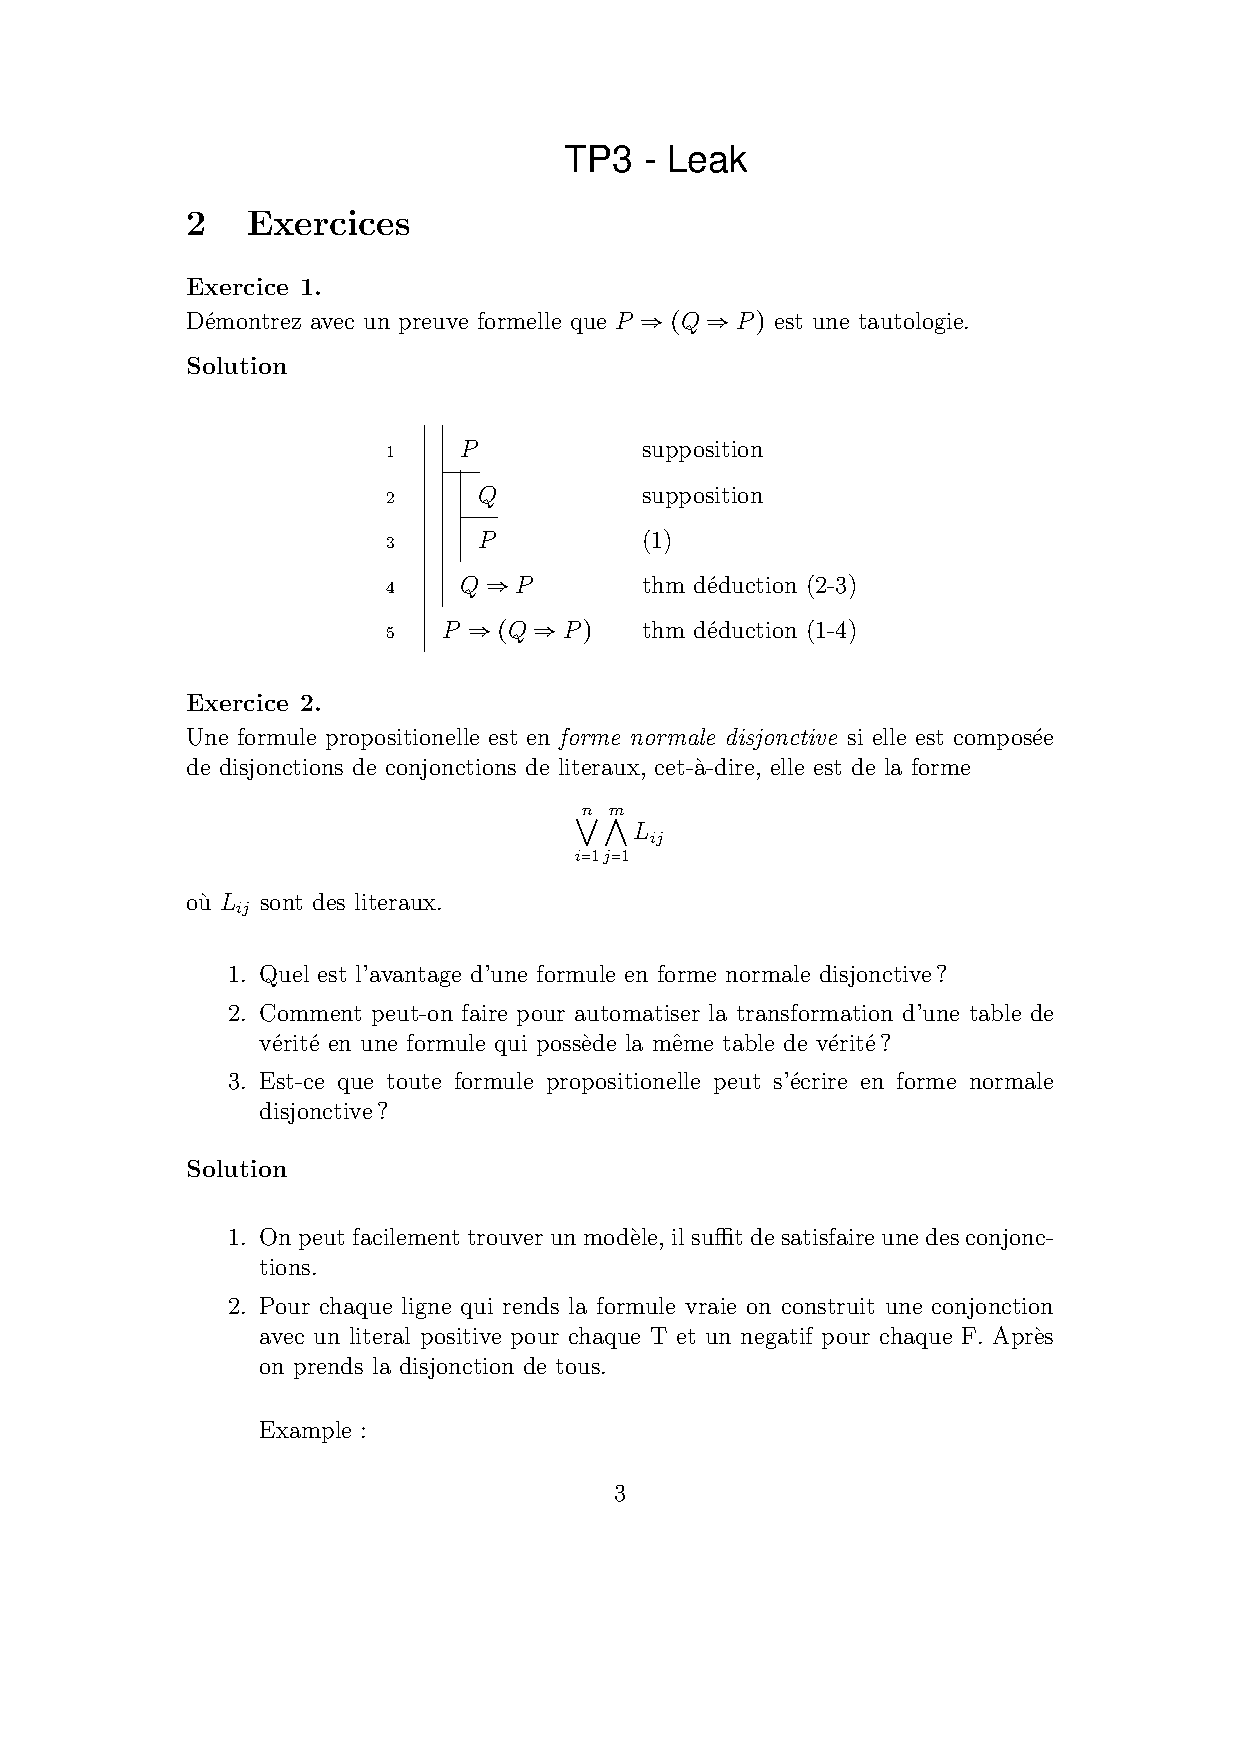
\includepdf[pages=-]{TP3_SOL_CUT.pdf}
  
  \chapter*{TP 4}
\addcontentsline{toc}{chapter}{TP 4}


% \newpage

% \section*{Rappel}

% \textbf{Forme normale conjonctive (FNC):} \\

% $$
% \bigwedge_{i = 1}^n \bigvee_{j = 1}^{m_i} L_{ij}
% $$

% avec $L_{ij}$ litéral, cet-à-dire, une proposition primaire (ex. $A$) ou sa négation (ex. $\neg A$). \\

% \textbf{Example:}

% $$
% (\neg A \vee B) \wedge (B \vee C) \wedge (\neg B \vee C \vee \neg D)
% $$

% \vspace{0.5cm}

% \textbf{Algorithme de normalisation:} \\

% \begin{enumerate}
%  \item Eliminer les $\Rightarrow$ et $\Leftrightarrow$ en les remplaçant par des formules équivalentes a l'aide des lois de l'implication et
%  de l'équivalence. 
%  $$
%  p \Rightarrow q \loeq \neg p \vee q \quad \text{et} \quad p \Leftrightarrow q \loeq (p \Rightarrow q) \wedge (q \Rightarrow p)
%  $$
 
%  \item Déplacer les négations vers l'intérieur et utilisant les lois de De Morgan.
 
%  \item Déplacer les disjonctions ($\vee$) vers l'intérieur en utilisant les lois distributives.
 
%  \item Simplifier en éliminant les formes ($P \vee \neg P$) dans chaque disjonction.
 
% \end{enumerate}

% \vspace{0.5cm}

% \textbf{Règle de résolution:} \\

% \begin{tabular}{l}
% $p_1 \vee p_2 \vee \ldots \vee p_{i - 1} \vee c \vee p_{i + 1} \vee \ldots \vee p_n$ \\
% $q_1 \vee q_2 \vee \ldots \vee q_{j - 1} \vee \neg c \vee q_{j + 1} \vee \ldots \vee q_m$ \\
% \hline
% $p_1 \vee \ldots \vee p_{i - 1} \vee p_{i + 1} \vee \ldots \vee p_n \vee q_1 \vee \ldots \vee q_{j - 1} \vee q_{j + 1} \vee \ldots \vee q_m$ 
% \end{tabular}

% \vspace{0.5cm}

% \textbf{Example:}

% \begin{tabular}{l}
% $p \vee \neg q $ \\
% $\neg r \vee q$ \\
% \hline
% $p \vee \neg r$ 
% \end{tabular}

% \newpage

% \textbf{Algorithme de résolution:} \\

% \begin{enumerate}
%  \item Mettre les prémisses et la négation en FNC dans $S$
%  \item Tant que \textbf{false} $\notin S$ et qu'il existent $p, q$ résolvables, non résolues
%  \begin{enumerate}
%   \item Apliquer la résolution sur $p$ et $q$
%   \item Ajouter le résultat dans $S$
%  \end{enumerate}
%   \item Si \textbf{false} $\in S$ alors c'est prouvé
%   \item Sinon il n'y a pas de preuve
% \end{enumerate}

% \vspace{0.5cm}

% \textbf{Propriétés de l'algorithme:} \\

% Soit $P = \{p_1, \ldots p_n \}$ l'ensemble de prémisses et $c$ une proposition. \\

% \textit{Soundness (adéquat):} Si $P \vdash c$ alors $P \models c$ 

% \textit{Completeness (complet):} Si $P \models c$ alors $P \vdash c$

% \textit{Decidable (décidable):} L'algorithme se termine après un nombre fini d'étapes.

% \newpage

% \section*{Exercices}

\subsection*{Exercice 1}
Prouvez que la régle de résolution est valide.

\paragraph*{NB:} Règle de résolution : 
 \begin{tabular}{l}
 $p_1 \vee p_2 \vee \ldots \vee p_{i - 1} \vee c \vee p_{i + 1} \vee \ldots \vee p_n$ \\
 $q_1 \vee q_2 \vee \ldots \vee q_{j - 1} \vee \neg c \vee q_{j + 1} \vee \ldots \vee q_m$ \\
 \hline
 $p_1 \vee \ldots \vee p_{i - 1} \vee p_{i + 1} \vee \ldots \vee p_n \vee q_1 \vee \ldots \vee q_{j - 1} \vee q_{j + 1} \vee \ldots \vee q_m$ 
 \end{tabular}

 \vspace{0.5cm}

    \subsubsection*{Solution}

La règle de résolution peut s'écrire comme suit :

\begin{center}
\begin{tabular}{c}
$p \lor q$ \\
$r \lor \neg q$\\
\hline
$p \lor r$\\
\end{tabular}\\
\end{center}

Elle peut être démontrée de la manière suivante :

\begin{tabular}{|l|l|}
\hline
1. $p \lor q$ & prémisse \\
2. $r \lor \neg q$ & prémisse \\
\indent 3. $\neg (p \lor r)$ & supposition \\
\indent 4. $\neg p \land \neg r$ & De Morgan 2 \\ 
\indent 5. $\neg p$ & simplification \\
\indent 6. $q$ & syllogisme disjoint (1, 5) \\
\indent 7. $\neg r$ & simplification (4)\\
\indent 8. $\neg q$ & syllogisme disjoint (2, 7) \\
9. $\neg (\neg (p \lor r))$ & contradiction (3) \\
10. $p \lor r$ & négation \\
\hline
\end{tabular}

\subsection*{Exercice 2}
Est-ce que cette application de la règle de résolution est correcte? Justifiez.
$$
res(P \vee Q, \neg P \vee \neg Q) = \textbf{false}
$$

    \subsubsection*{Solution}
    
res($P \lor Q$, $\neg P \lor \neg Q$) = \textbf{false} n'est pas une application valable de la règle de résolution.\\
En effet, si on prend $R$ tel que $R \Lleftarrow\!\!\!\!\Rrightarrow \neg P$, on peut appliquer :
\begin{center}
\begin{tabular}{c}
$P \lor Q$ \\
$R \lor \neg Q$\\
\hline
$P \lor R$\\
\end{tabular}\\
\end{center}
On obtient donc $P \lor R$.
Or $(P \lor R) \Lleftarrow\!\!\!\!\Rrightarrow (P \lor \neg P)$.
Puisque $(P \lor \neg P)$ est toujours vrai, on en conclut que res($P \lor Q$, $\neg P \lor \neg Q$) = \textbf{true}.

\subsection*{Exercice 3}
Pour chaque ensemble de prémisses montrez avec l'algorithme de résolution que la conclusion est une conséquence logique des prémisses.
\begin{enumerate}
 \item 
 Prémisses: $P \Rightarrow Q, Q \Rightarrow R$ \\
 Conclusion: $P \Rightarrow R$
 \item
 Prémisses: $P \vee Q, P \Rightarrow R, Q \Rightarrow R$ \\
 Conclusion: $R$
 \item
 Prémisses: $(P \Leftrightarrow Q) \Leftrightarrow R, P$ \\
 Conclusion: $Q \Leftrightarrow R$
 \item
 Prémisses: $P \Rightarrow Q, R \Rightarrow T, Q \vee T \Rightarrow U, \neg U$ \\
 Conclusion: $\neg P \wedge \neg R$
 \item
 Prémisses: $\neg P \Rightarrow (Q \Rightarrow R), T \vee \neg R \vee U, P \Rightarrow T, \neg T$ \\
 Conclusion: $Q \Rightarrow U$
\end{enumerate}

    \subsubsection*{Solution}
  
    \subsection*{Rappel : Algorithme de résolution}
    
        \begin{enumerate}
            \item On met les prémisses et la $\neg$ conclusion en FNC
            \item $While(false \notin S$ AND p q resolvable)
            \begin{itemize}
                \item Résolution sur p et q
                \item Ajouter résultat dans S
            \end{itemize}
            \item Si $false \in S \rightarrow Proof$
            \item Sinon $\rightarrow No proof $
        \end{enumerate}
        
    \subsection*{1.}
    
    \begin{table}[H]
        \centering
        %\caption{My caption}
        \label{my-label}
        \begin{tabular}{lll}
        $ p \Rightarrow q$ & \textbf{Conversion} & $ \neg p \lor q $  \\
        $ q \Rightarrow r$ &                     & $ \neg q \lor r $  \\ \cline{1-1} \cline{3-3} 
        $ p \Rightarrow r$ &                     & $ p \land \neg r $
        \end{tabular}
    \end{table}
    
    
    \begin{flalign*}
        &S = \left \{ \neg p \lor q, \neg q \lor r,    
        \neg r \right \} &\\
        & res \left (\neg p \lor q, \neg q \lor r \right ) = \neg p \lor r &\\
        &S = \left \{ \neg p \lor q, \neg q \lor r, p \land \neg r , \neg p \lor r \right \}&\\
        & res \left (\neg p \lor r, \neg r \right ) = \neg p &\\
        &S = \left \{ \neg p \lor q, \neg q \lor r, p \land \neg r , \neg p \lor r, \neg p \right \}&\\
        & res \left (\neg p , p \right ) = \textbf{false} &\\
    \end{flalign*}
    
    $p \Rightarrow r$ est une conséquence logique des prémisses.\\
        
        
    \subsection*{2.}
    
    On convertit les prémisses, et on les ajoute dans S (ainsi que $\lnot \text{conclusion}$).\\
    
    \begin{flalign*}
        &S = \left\{ P \lor Q, \lnot P \lor R, \lnot Q \lor R, \lnot R, P\right\} &\\
        & res \left (P \lor Q,  \lnot P \lor R \right ) = Q \lor R &\\
        &S = \left\{ Q \lor R, \lnot Q \lor R, \lnot R \right\} &\\
        & res \left (Q \lor R, \lnot Q \lor R, \right ) = R \lor R = R &\\
        &S = \left\{ R, \lnot R \right\} &\\
        & res \left (R, \lnot R \right ) = \textbf{false} &\\
    \end{flalign*}
    
    $R$ est une conséquence logique des prémisses.\\
        


\subsection*{Exercice 4}
Demontrez que $p_1 \wedge \ldots \wedge p_n \models c$ si et seulement si $p_1 \wedge \ldots \wedge p_n \wedge \neg c \models \textbf{false}$.

    \subsubsection*{Solution}

\noindent \fbox{$\implies$} Par hypothèse, tous les modèles de $p_1 \wedge \ldots \wedge p_n$ sont des modèles de $c$. Autrement dit, $c$ est vraie à chaque fois que  $p_1,p_2,...,p_n$ sont vrais en même temps. Par conséquent, la formule $p_1 \wedge \ldots \wedge p_n \wedge \neg c$ est fausse pour tous les modèles de $p_1 \wedge \ldots \wedge p_n$. Autrement dit, $p_1 \wedge \ldots \wedge p_n \wedge \neg c$ n'a aucun modèle ou $p_1 \wedge \ldots \wedge p_n \wedge \neg c \models \textbf{false}$. \\

\noindent \fbox{$\impliedby$} Soit $M$ un modèle quelconque de  $p_1 \wedge \ldots \wedge p_n$. Puisqu'il n'y a aucun modèle pour  $p_1 \wedge \ldots \wedge p_n \wedge \neg c$, $c$ doit être vraie dans $M$ pour satisfaire le membre de droite. Autrement dit, tous les modèles de $p_1 \wedge \ldots \wedge p_n$ sont des modèles de $c$ ou $p_1 \wedge \ldots \wedge p_n \models c$.
  \chapter*{TP 5}
\addcontentsline{toc}{chapter}{TP 5}

% \section*{Rappel}

% \begin{enumerate}
% \item $\forall x \ p(x) \land q(x) \Lleftarrow\!\!\!\!\Rrightarrow (\forall x \ p(x)) \land (\forall x \ q(x))$
% \item $\exists x \ p(x) \vee q(x) \Lleftarrow\!\!\!\!\Rrightarrow (\exists x \ p(x)) \vee (\exists x \ q(x))$
% \item $\neg \exists x \ p(x) \Lleftarrow\!\!\!\!\Rrightarrow \forall x \ \neg p(x)$
% \item $\neg \forall x \ p(x) \Lleftarrow\!\!\!\!\Rrightarrow \exists x \ \neg p(x)$
% \item $(\forall x \ p(x)) \vee (\forall x \ q(x)) \Rrightarrow \forall x \ p(x) \vee q(x)$
% \item $\exists x \ p(x) \land q(x) \Rrightarrow (\exists x \ p(x)) \land (\exists x \ q(x))$
% \item $\exists x \ p(y) \land q(x) \Rrightarrow p(y) \land (\exists x \ p(x))$
% \item $\exists x, y \ p(x, y) \Rrightarrow \exists y, x \ p(x, y)$
% \end{enumerate}


% \newpage


% \section*{Exercices}


\subsection*{Exercice 1}
Expliquez ce qu'est un modèle en logique des prédicats. 

    \subsubsection*{Solution}
    
    Un modèle est une interprétation qui rend toutes les formules vraies.
    
    Soit un ensemble de formules $B=\{p_1,\dots ,p_n\}$, une interprétation $I$ de B est un \textit{modèle} si et seulement si $\forall p_i \in B:VAL_I(p_i) = \text{True}$

\subsection*{Exercice 2}
Soit l'interprétation suivante:
\begin{center}
\begin{tabular}{r l}
$D_I$ & $= \mathbb{N}$ \\
$val_I(a)$ & $= 0$ \\
$val_I(f)$ & $= $ \ ''succ`` \\
$val_I(P)$ & $= $ \ ''$<$`` \\
$val_I(x)$ & $= 1$ \\
$val_I(y)$ & $= 0$ \\
\end{tabular}
\end{center}
Déterminez les valeurs de vérité des formules suivantes dans cette interprétation:
\begin{enumerate}
\item $P(x, a)$
\item $P(x, a) \land P(x, f(x))$
\item $\exists y \ P(y, x)$
\item $\exists y \ P(y, a) \vee P(f(y), y)$
\item $\forall x \ \exists y \ P(x, y)$
\item $\exists y \ \forall x \ P(x, y)$
\end{enumerate}

    \subsubsection*{Solution}
    
    {\setlength{\baselineskip}{1.3\baselineskip} %% CONTROLE L'INTERLIGNE (la commande englobe tout le chunk et se termine avec "\par}"
    
    \paragraph{1)}

    $VAL_I(P(x,a)) = T$
    \\
    \texttt{ssi} $val_I(P)(VAL_I(x),VAL_I(a)) = T$
    \\
    \texttt{ssi} $val_I(P)(val_I(x),val_I(a)) = T$
    \\
    \texttt{ssi} $val_I(x) < val_{I}(a) = T$
    \\
    \texttt{ssi} $1<0$    
    \\
    \texttt{or} $1<0 = F$
    \\
    $\Rightarrow VAL_I(P(x,a)) = $\texttt{ False} 
    
    \paragraph{2)}


    $VAL_I[P(x,a) \land P(x, f(x))] = T$
    \\
    \texttt{ssi} $VAL_I(P(x,a)) \land VAL_I(P(x,f(x))) = T$
    \\
    \texttt{or} $VAL_I(P(x,a)) = $\texttt{ False} 
    \\
    $\Rightarrow VAL_I[P(x,a) \land P(x, f(x))] = $\texttt{ False} 

    \paragraph{3)}
    
    
    $VAL_I(\exists y P(y,x)) = T$
    \\
    \texttt{ssi} $\exists d\in \mathbb{N}: VAL_{I'}(P(y,x)) = T$ où $I' = I\{y\rightarrow d\}$
    \\
    \texttt{ssi} $\exists d\in \mathbb{N}: val_{I'}(P)(VAL_{I'}(y),VAL_{I'}(x)) = T$
    \\
    \texttt{ssi} $\exists d\in \mathbb{N}: val_{I'}(P)(val_{I'}(y),val_{I'}(x)) = T$ 
    \\
    \texttt{ssi} $\exists d\in \mathbb{N}: d < 1$. 
    \\
    $\Rightarrow VAL_I(\exists y P(y,x)) = $\texttt{ True}, si $d=0$
    

    \paragraph{4)}
    $VAL_I[\exists x \ P(y,a)\lor P(f(y), y)] = T$ 
    \\
    \texttt{ssi} $\exists d\in D_{I}:VAL_{I'}[P(y,a)\lor P(f(y),y)] = T$ avec $I' = I \{y \rightarrow d\}$
    \\
    \texttt{ssi} $\exists d\in D_{I}:VAL_{I'}[P(y,a)]\lor VAL_{I'}[P(f(y),y)] = T$
    \\
    \texttt{ssi} $\exists d\in D_{I}:val_{I'}(P)[val_{I'}(y), val_{I'}(a)]\lor val_{I'}(P)[VAL_{I'}(f(y)), val_{I'}(y)] = T$
    \\
    \texttt{ssi} $\exists d\in D_{I}:(d<0)\lor [val_{I'}(f)(val_{I'}(y)) < d]$
    \\%coucouuu heyy
    \texttt{ssi} $\exists d\in \mathbb{N}:(d<0)\lor (succ(d) < d)$
    \\
    \texttt{ssi} $\exists d\in \mathbb{N}: (d<0)\lor (d+1 < d)$
    \\
    $\Rightarrow  VAL_I[\exists P(y,a)\lor P(f(y), y)] = $\texttt{ False} 

    \paragraph{5)}
    $VAL_I[\forall x \exists y P(x,y)] = T$
    \\
	$\forall d\in \mathbb{N}, VAL_{I'}[\exists yP(x,y)] = T$ avec $I' = I\{x \rightarrow d\}$
	\\
	$\forall d\in \mathbb{N} \exists e \in \mathbb{N} : VAL_{I''}[P(x,y)] = T$ avec $I'' = I'\{y \rightarrow e\}$
	\\
	$\forall d\in \mathbb{N} \exists e \in \mathbb{N} : val_{I''}(P)[val_{I''}(x), val_{I''}(y)] = T$
	\\
	$\forall d\in \mathbb{N} \exists e \in \mathbb{N} : d<e$ 
	\\
	Si on prend e = d+1 $\in \mathbb{N}$, on a d < d + 1 ce qui est vrai $\forall d \in \mathbb{N}$
	\\
	$\Rightarrow  VAL_I[\forall x \exists y P(x,y)] = $\texttt{ True}
	
    \paragraph{6)}
    $VAL_I[\exists y \forall x P(x,y)] = T$
    \\
	$\exists d\in \mathbb{N}, VAL_{I'}[\forall xP(x,y)] = T$ avec $I' = I\{y \rightarrow d\}$
	\\
	$\exists d\in \mathbb{N} \forall e \in \mathbb{N} : VAL_{I''}[P(x,y)] = T$ avec $I'' = I'\{x \rightarrow e\}$
	\\
	$\exists d\in \mathbb{N} \forall e \in \mathbb{N} : val_{I''}(P)[val_{I''}(x), val_{I''}(y)] = T$
	\\
	$\exists d\in \mathbb{N} \forall e \in \mathbb{N} : d<e$ 
	\\
	Si on prend e = 0, on a d < 0 ce qui n'est vrai pour aucun $d \in \mathbb{N}$
	\\
	$\Rightarrow  VAL_I[\exists y \forall x P(x,y)] = $\texttt{ False}

    \par} %% NE PAS EFFACER
          %% SINON QUOI HEIN??

\subsection*{Exercice 3}
On considère une grille $3 \times 3$ et 
$$
P = \{(1, 1), (1, 2), (1, 3), (2, 1), (2, 2), (2, 3), (3, 1), (3, 2), (3, 3) \}
$$
l'ensemble des positions de la grille. De plus, on considère les prédicats $\t{carre}, \t{circle}, \t{vide}$ et $\t{adj}$ 
qui représentent les choses suivantes:
\vspace{0.2cm}
\begin{center}
\begin{tabular}{| l l |}
\hline
carre$(x)$ & la forme de la position $x$ est un carré. \\
circle$(x)$ & la forme de la position $x$ est un cercle. \\
vide$(x)$ & la position $x$ est vide. \\
adj$(x, y)$ & les positions $x$ et $y$ sont adjacentes \\
\hline
\end{tabular}
\end{center}
\vspace{0.2cm}

Pour chaque configuration, dites quelles sont les formules vraies.

\begin{center}
\begin{tabular}{ c c c c c }

A 
\begin{tabular}{|c|c|c|}
 \hline
 $\bigcirc$ & & \\ 
 \hline
 $\Box$ & & \\
 \hline
  & & $\bigcirc$ \\
 \hline
\end{tabular}

&

B
\begin{tabular}{|c|c|c|}
 \hline
 $\Box$ & & \\ 
 \hline
 $\bigcirc$ &$\Box$ & \\
 \hline
  & &$\Box$ \\
 \hline
\end{tabular}

&
C
\begin{tabular}{|c|c|c|}
 \hline
  & $\Box$ & \\ 
 \hline
 $\Box$ & & $\Box$ \\
 \hline
  & $\Box$ & \\
 \hline
\end{tabular}

&

D
\begin{tabular}{|c|c|c|}
 \hline
 $\bigcirc$ & $\Box$ & $\bigcirc$ \\ 
 \hline
 $\Box$ & $\bigcirc$ & $\Box$ \\
 \hline
 $\bigcirc$ & $\Box$ & $\bigcirc$ \\
 \hline
\end{tabular}

&

E
\begin{tabular}{|c|c|c|}
 \hline
 $\bigcirc$ &  & $\Box$ \\ 
 \hline
 $\Box$ & $\bigcirc$ & $\Box$ \\
 \hline
 $\Box$ & $\Delta$ & $\bigcirc$ \\
 \hline
\end{tabular}

\end{tabular}
\end{center}


\begin{enumerate}
  \item $\exists x : P \ \t{vide}(x)$
  \item $\exists x : P \ \neg \t{vide}(x)$
  \item $\exists x : P \ \t{circle}(x)$
  \item $\exists x : P \ \t{carre}(x)$
  \item $\forall x : P \ \t{vide}(x) \vee \t{carre}(x) \vee \t{circle}(x)$
  \item $\forall x : P \ \t{carre}(x) \Rightarrow \exists y : P \ (\t{adj}(x, y) \land \t{circle}(y))$
  \item $\forall x : P \ \t{carre}(x) \Rightarrow \exists y : P \ (\t{adj}(x, y) \land \t{carre}(x))$
  \item $\exists x, y, z : P \ \t{vide}(x) \land \t{vide}(y) \land \t{vide}(z)$
  \item $\exists x : P \ (\forall x : P \ \t{circle}(x)) \vee \t{carre}(x)$
  \item $\forall x : P \ \exists y : P \ \neg \t{vide}(x) \land \t{vide}(y)$
  \item $\forall x : P \ \exists y : P \ \t{vide}(x) \land \neg \t{vide}(y)$
  \item $\forall x : P \ \exists y : P \ \neg \t{vide}(x) \Rightarrow \t{vide}(y)$
  \item $\forall x : P \ \exists y : P \ \neg \t{vide}(y) \Rightarrow \t{vide}(x)$
  \item $\forall x : P \ \t{circle}(x) \Rightarrow \exists y, z : P \ \t{carre}(y) \land \t{carre}(z) \land \t{adj}(x, y) \land \t{adj}(x, z)$
  \item $\exists x : P \ \t{vide}(x) \Rightarrow (\forall y : P \ \neg \t{vide}(x) \Rightarrow \t{carre}(y)$)
 \end{enumerate}

    \subsubsection{Solution}

    \begin{itemize}
        \item \textbf{A :} 1, 2, 3, 4, 5, 6, 8 , 9, 10, 11, 12, 13
        \item \textbf{B :} 1, 2, 3, 4, 5, 8, 9, 10, 11, 12, 13, 14
        \item \textbf{C :} 1, 2, 4, 5, 8, 9 , 10, 11, 12, 13, 14, 15
        \item \textbf{D :} 2, 3, 4, 5, 6, 9, 14
        \item \textbf{E :} 1, 2, 3, 4, 7, 9, 10, 11, 12, 13
    \end{itemize}

\subsection*{Exercice 4}
Faites une preuve formelle de:

\begin{enumerate}

	\item \enter
\begin{flushleft}
\begin{tabular}{l}
$\exists x \ p(x)$ \\
$\forall x \ p(x) \Rightarrow q(x)$ \\
\hline
$\exists x \ q(x)$
\end{tabular}
\end{flushleft}

	\item \enter
\begin{flushleft}
\begin{tabular}{l}
$\forall x \ p(x) \vee r(x) \Rightarrow \neg q(x)$ \\
$\exists x \ \neg (\neg p(x) \land \neg r(x))$ \\
\hline
$\exists x \ \neg q(x)$
\end{tabular}
\end{flushleft}

	\item \enter
\begin{flushleft}
\begin{tabular}{l}
$\forall x \ p(x) \vee q(x) \Rightarrow r(x) \land s(x)$ \\
$\neg \forall x \ r(x) \land s(x)$ \\
\hline
$\neg \forall x \ p(x)$
\end{tabular}
\end{flushleft}

\newpage

	\item \enter
\begin{flushleft}
\begin{tabular}{l}
$\forall x \ q(x) \vee s(x) \Rightarrow r(x) $ \\
$\neg \forall z \ p(z) \vee \neg s(z)$ \\
\hline
$\exists x \ r(x)$
\end{tabular}
\end{flushleft}

	\item \enter
\begin{flushleft}
\begin{tabular}{l}
$\forall x \ p(x) \Rightarrow \neg q(x)$ \\
$\exists x \ r(x) \land q(x)$ \\
\hline
$\exists x \ r(x) \land \neg p(x)$
\end{tabular}
\end{flushleft}

	\item \enter
\begin{flushleft}
\begin{tabular}{l}
$p(a)$ \\
$\forall x \ p(x) \Rightarrow q(x, b)$ \\
\hline
$\exists x \ q(a, x)$
\end{tabular}
\end{flushleft}

	\item \enter
\begin{flushleft}
\begin{tabular}{l}
$\forall x \ \forall y \ p(x, y)$ \\
\hline
$\exists x \ p(x, x)$
\end{tabular}
\end{flushleft}

	\item \enter
\begin{flushleft}
\begin{tabular}{l}
$\forall x \ \neg p(x, x) \land \forall x \ \forall y \ \forall z \ p(x, y) \land p(y, z) \Rightarrow p(x, z)$ \\
\hline
$\forall x \ \forall y \ \neg (p(x, y) \land p(y, x))$
\end{tabular}
\end{flushleft}

\end{enumerate}


    \subsubsection{Solution}
    
        \paragraph{1}
        
            \begin{tabular}{|l|l|}
            \hline
            1. $\exists x \  p(x)$ & prémisse \\
            2. $\forall x \  p(x) \Rightarrow q(x)$ & prémisse \\
            3. $p(a)$ & $\exists$ élim(1) \\
            4. $p(a) \Rightarrow q(a)$ & $\forall$ élim(2) \\ 
            5. $q(a)$ & Modus ponens(3,4) \\
            6. $\exists x \  q(x)$ & intro(5) \\
            \hline
            \end{tabular}
        
        \paragraph{2}
        
            \begin{tabular}{|l|l|}
            \hline
            1. $\forall x \  p(x) \lor r(x) \Rightarrow \neg q(x)$ & prémisse \\
            2. $\exists x \  \neg (\neg p(x) \land \neg r(x))$ & prémisse \\
            3. $\exists x \  p(x) \lor r(x)$ & DeMorgan(2) \\
            4. $p(a) \lor r(a)$ & $\exists$ élim(3) \\ 
            5. $p(a) \lor r(a) \Rightarrow \neg q(a)$ & $\forall$ élim(1) \\
            6. $\neg \ q(a)$ & Modus ponens (4,5)\\
            7. $\exists x \  \neg q(x)$ & $\exists intro(6)$\\
            \hline
            \end{tabular}
            
        \paragraph{3}
            \begin{tabular}{|l|l|}
            \hline
            1. $ \forall x \ p(x) \lor q(x) \Rightarrow r(x) \land s(x) $ & prémisse \\
            2. $ \lnot \forall x \ r(x) \land s(x) $ & prémisse \\
            3. $ \exists x \ \neg  (r(x) \land s(x)) $ & "rentrer" négation (2) \\
            4. $ \neg r(a) \lor \neg s(a) $ & $\exists$ élim + DeMorgan (3) \\
            5. $ p(a) \lor q(a) \Rightarrow r(a) \land s(a) $ & $\forall$ élim(1) \\
            6. $ \neg (p(a) \lor q(a)) $ & Modus Tollens (5,4) \\
            7. $ \neg p(a) \land \neg q(a) $ & DeMorgan(6) \\
            8. $ \neg p(a) $ & Simplif(7)\\
            9. $ \exists x \ \neg p(x) $ & $\exists$ Intro(8) \\
            10. $ \neg \forall x \ p(x) $ & "mis en avant" négation (9)\\
            \hline
            \end{tabular}
        
        
        \paragraph{4}
            
            \begin{tabular}{|l|l|}
            \hline
            1. $\forall x \  q(x) \lor s(x) \Rightarrow r(x)$ & prémisse\\
            2. $\neg \forall z \  p(z) \lor \neg s(z)$ & prémisse\\
            3. $\exists z \  \neg (p(z) \lor \neg s(z))$ & prémisse\\
            4. $\exists z \  \neg p(z) \land s(z)$ & DeMorgan(3)\\
            5. $\neg p(a) \land s(a)$ & $\exists$ élim(4)\\
            \indent 6. $\neg \exists x \  r(x)$ & hypothèse\\
            \indent 7. $\forall x \neg r(x)$ & (6)\\
            \indent 8. $\neg r(a)$ & $\forall$ elim(7) \\
            \indent 9. $q(a) \lor s(a) \Rightarrow r(a) $ & $\forall$ elim(1) \\
            \indent 10. $ \neg (q(a) \lor s(a)) $ & Modus Tolens(8,9) \\
            \indent 11. $ \neg q(a) \land \neg s(a) $ & DeMorgan (10) \\
            \indent 12. $ \neg s(a) $ & Simplification(11) \\
            \indent 13. $ s(a) $ & Simplification(5) \\
            14. $\neg \neg \exists x \ r(x) $ &  Réduction à l'absurde(6-13) \\
            15. $\exists x \ r(x) $ & Double négation (14)\\
                    
            \hline
            \end{tabular}
            
            
        \paragraph{5}
            
            \begin{tabular}{|l|l|}
            \hline
            1. $ \forall x \ p(x) \Rightarrow \neg q(x) $ & prémisse\\
            2. $ \exists x \ r(x) \land \neg q(x) $ & prémisse\\
            3. $ r(a) \land \neg q(a) $ & $\exists$ élim(2)\\
            4. $ p(a) \Rightarrow \neg q(a) $ & $\forall$ élim(1)\\
            \indent 5. $ p(a) $ & Hypothèse \\
            \indent 6. $ \neg q(a) $ & Modus Ponens (4,5) \\
            \indent 7. $ q(a) $ & Simplif(3) \\
            8. $ \neg p(a) $ & Réduction à l'absurde (5-7)\\
            9. $ r(a) $ & Simplif (3) \\
            10. $ r(a) \land \neg p(a) $ & conjonction (8,9)\\
            11. $ \exists x \ r(x) \land \neg p(x) $ & $\exists$ Intro(10) \\
            
            \hline
            \end{tabular}
            
        \paragraph{6}
            
            \begin{tabular}{|l|l|}
            \hline 
            1. p(a) & prémisse \\
            2. $ \forall x \ p(x) \Rightarrow q(x,b) $ & prémisse \\
            3. $ p(a) \Rightarrow q(a,b) $ & $\forall$ Elim(2) \\
            4. $ \neg p(a) \lor q(a,b) $ & loi implication (3) \\
            5. $ q(a,b) $ & syllogisme disjoint (1,4) \\
            6. $ \exists x \ q(a,x) $ & $\exists$ Intro(5) \\
            \hline
            \end{tabular}
            
             
        \paragraph{7}
            
            \begin{tabular}{|l|l|}
            \hline   
            1. $\forall x \ \forall y \ p(x,y)  $ & prémisse \\
            2. $ p(a,a) $ & 2x $\forall$ Elim(1) \\
            3. $ \exists x \ p(x,x) $ & $\exists$ Intro(2) \\
             \hline
            \end{tabular}
            
            
         \paragraph{8}
            
            \begin{tabular}{|l|l|}
            \hline   
            1. $ (\forall x \ \neg p(x,x)) \land (\forall x \  \forall y \  \forall z \ p(x,y) \land p(y,z) \Rightarrow p(x,z)) $ & prémisse \\
            \indent 2. $ \neg \forall x \  \forall y \ \neg (p(x,y) \land p(y,x))  $ & Hypothèse \\
            \indent 3. $  \exists x \  \exists y \ \neg \neg (p(x,y) \land p(y,x))  $ & "rentrer" négation(2) \\
            \indent 4. $  \exists x \  \exists y \ (p(x,y) \land p(y,x))  $ & double négation(3) \\
            \indent 5. $  p(a,b) \land p(b,a) $ & 2x $\exists $ élim(4) \\
            \indent 6. $  \forall x \  \forall y \  \forall z \ p(x,y) \land p(y,z) \Rightarrow p(x,z) $ & Simplif(1) \\
            \indent 7. $  p(a,b) \land p(b,a) \Rightarrow p(a,a) $ & 3x $\forall$ Elim(6) [$x\rightarrow a ; y\rightarrow b ; z\rightarrow a $] \\
            \indent 8. $ p(a,a) $ & Modus Ponens(5,7) \\
            \indent 9. $ \forall x \ \neg p(x,x) $ & Simplif(1) \\
            \indent 10. $ \neg p(a,a) $ & $\forall$ Elim(9)  \\
            10. $ \neg \neg \forall x \  \forall y \ \neg (p(x,y) \land p(y,x))  $ & Réduction à l'absurde (2-10) \\
            11. $ \forall x \  \forall y \ \neg (p(x,y) \land p(y,x))  $ & double négation \\
            
            
            \hline
            \end{tabular}
            
            
            
            
            
            
            
            
  \chapter*{TP 6}
\addcontentsline{toc}{chapter}{TP 6}

\subsection*{Exercice 1}
Pour chacune des affirmations suivantes, démontrez-la ou trouvez un contre-exemple.
\begin{enumerate}
	\item $\neg \exists x \ \forall y \ p(x, y) \Lleftarrow\!\!\!\!\Rrightarrow \forall x, y \ \neg p(x, y)$
	\item $\exists x \ p(x) \vee q(x) \Rrightarrow (\exists x \ p(x)) \vee (\exists x \ q(x))$
	\item $(\exists x \ p(x)) \wedge (\exists x \ q(x)) \Rrightarrow \exists x \ p(x) \wedge q(x)$
	\item $\forall x \ \exists y \ p(x, y) \Lleftarrow\!\!\!\!\Rrightarrow \exists x \forall y \ p(x, y)$
	\item $(\exists x \ p(x)) \vee (\exists x \ q(x)) \Rrightarrow \exists x \ p(x) \vee q(x)$
\end{enumerate}

    \subsubsection*{Solution}
  
    \paragraph{1)}  
        \begin{tabular}{|l|l|}
        \hline
        $\forall$ x $\neg$ $\forall$ y p(x,y) $\Lleftarrow \Rrightarrow$ $\forall$ x,y $\neg$ p(x,y) & $\neg$ vers l'intérieur\\
        $\forall$ x $\exists$ y $\neg$ p(x,y) $\ne$ $\forall$ x,y $\neg$ p(x,y)& $\neg$ vers l'intérieur\\
        \hline
        \end{tabular}
    
    \paragraph{2)}
        \begin{tabular}{|l|l|}
        \hline
        1. $\exists$x p(x) $\lor$ q(x) & hypothèse \\
        $\qquad$ 2. $\neg$ [$\exists$x p(x) $\lor$ $\exists$x q(x)] & hypothèse absurde\\
        $\qquad$ 3. $\neg$ $\exists$x p(x) $\land$ $\neg$ $\exists$x q(x) & Morgan\\
        $\qquad$ 4. $\forall$x $\neg$ p(x) $\land$ $\forall$x $\neg$ q(x) & $\neg$ vers l'intérieur\\
        $\qquad$ 5. $\forall$x $\neg$ p(x) & simplification\\
        $\qquad$ 6. $\neg$ p(x) & élimination $\forall$\\
        $\qquad$ 7. p(x) $\lor$ q(x) & élimination $\exists$ (1)\\
        $\qquad$ 8. q(x) & Syllogisme disjoint (6,7)\\
        $\qquad$ 9. $\forall$x $\neg$ q(x) & simplification (4)\\
        $\qquad$ 10. $\neg$ q(x) & \\
        11. $\neg \neg$ ( $\exists$x p(x) $\lor$ $\exists$x q(x)) & Preuve par contradiction\\
        12. $\exists$x p(x) $\lor$ $\exists$x q(x)& Simplification\\
        13. $\exists$x p(x) $\lor$ q(x) $\Rrightarrow$ ($\exists$x p(x) $\lor$ ($\exists$x q(x)) & Preuve\\
        \hline
        \end{tabular}
        
    \paragraph{3)}
        Faux, par exemple soit p(x) = x est petit;
        soit q(x) = x est grand. Il existe un $x$ petit, et il existe un $x$ grand, mais pas de $x$ petit et grand à la fois. Il s'agit ici de comprendre que dans le premier cas, la variable $x$ n'est pas la même à cause de la portée de deux quantificateurs, alors que dans le second, c'est bien le même $x$.
        
    \paragraph{4)}
        Faux, par exemple:
        Soit P(x,y) = y est le père de x.
        Si pour tout $x$, il existe un $y$ tel que $y$ est le père de $x$, ce n'est pas pour autant qu'un $x$ aura pour père tous les $y$ possibles.
        
    \paragraph{5)}
        \begin{tabular}{|l|l|}
        \hline
        1. $(\exists xp(x)) \lor (\exists xq(x))$ & Prémisse \\
        \indent 2. $\neg \exists xp(x) \lor q(x)$ & Hypothèse absurde\\
        \indent 3. $\forall x\neg (p(x) \lor q(x))$ & Loi de la négation(2)\\
        \indent 4. $\forall x(\neg p() \land \neg q(x))$ & De Morgan(3) \\
        \indent 5. $\neg p(a) \land \neg q(a)$ & Élimination $\forall$(4) \\
        \indent 6. $\neg p(a)$ & Simplification(5) \\
        \indent 7. $\forall x(\neg p(x)) $ & Introduction $\forall$(6) \\
        \indent 8. $\neg \exists x p(x)$ & Loi de la négation(7) \\
        \indent 9. $\exists x q(x)$ & Syllogisme Disjoint(1, 6)\\
        \indent 10. $q(a)$ & Élimination $\exists$(9)\\
        \indent 11. $\neg q(a)$ & Simplification(5)\\
        12. $\neg \neg \exists xp(x) \lor q(x)$ & Réduction à l'absurde \\
        13. $\exists xp(x) \lor q(x)$ & Simplification(11)\\
        \hline
        \end{tabular}
        
\subsection*{Exercice 2}
Mettez les formules suivantes en forme normale prenexe puis en forme normale de Skolem et finalement en forme clausale. 
\begin{enumerate}
\item $(p(x) \vee \exists x \ q(x)) \Rightarrow \forall z \ r(z)$
\item $(\forall x \ (p(x) \Rightarrow q(x))) \wedge (\exists z \ p(z)) \wedge (\exists z \ (q(z) \Rightarrow r(t)))$
\item $\forall x \ ( ((\exists y \ r(x, y)) \wedge (\forall y \  \neg s(x, y)) \Rightarrow \neg (\exists y \ r(x, y) \wedge P)) )$
\item $\neg \forall x \ \exists y \ f(u, x, y) \Rightarrow (\exists x \ \neg \forall y \ g(y, v) \Rightarrow h(x))$
\end{enumerate}

    \subsubsection*{Solution}
    
    \paragraph{1)}
    \begin{center}
    \begin{tabular}{|l|l|c|}
    \hline
    $(p(x) \lor \exists x \ q(x)) \Rightarrow \forall z \ r(z)$ & Départ & Expression de base \\
    $\neg (p(x) \lor \exists x \ q(x)) \lor (\forall z \ r(z))$ & Suppression de $\Rightarrow$ & \\
    $\neg (p(y) \lor \exists x \ q(x)) \lor (\forall z \ r(z))$ & Renommage des variables & \\
    $(\neg p(y) \land \neg \exists x \ q(x)) \lor (\forall z \ r(z))$ & De Morgan 2 & \\
    $(\neg p(y) \land \forall x \ \neg q(x)) \lor (\forall z \ r(z))$ & $\neg \exists x$ devient  $\forall x \neg$ & \\
    $\forall x \ \forall z \ [(\neg p(y) \land \neg q(x)) \lor r(z)]$ & Extraction des quantificateurs & Forme prénexe\\
    $\forall x \ \forall z \ [(\neg p(y) \land \neg q(x)) \lor r(z)]$ & Pas de changements & Forme de Skolem\\
    $\forall x \ \forall z \ [(\neg p(y) \lor r(z)) \land (\neg q(x) \lor r(z))]$ & Distribution & Forme clausale\\
    \hline
    \end{tabular}
    \end{center}
    
    \paragraph{2)}
    
    \begin{center}
    \begin{tabular}{|l|l|c|}
    \hline
    $(\forall x \ (p(x) \Rightarrow q(x))) \land (\exists z \ p(z)) \land (\exists z \ (q(z) \Rightarrow r(t)))$ & Départ & Expression de base \\
    $(\forall x \ (\neg p(x) \lor q(x))) \land (\exists z \ p(z)) \land (\exists z \ (\neg q(z) \lor r(t)))$ & Suppression $\Rightarrow$ & \\
    $(\forall x \ (\neg p(x) \lor q(x))) \land (\exists y \ p(y)) \land (\exists z \ (\neg q(z) \lor r(t)))$ & Renommage & \\
    $\forall x \ \exists y \ \exists z \ [(\neg p(x) \lor q(x)) \land p(y) \land (\neg q(z) \lor r(t))]$ & Extraction & Forme prénexe \\
    $\forall x \ [(\neg p(x) \lor q(x)) \land p(f(x)) \land (\neg q(g(x)) \lor r(t))]$ & Élimination $\exists$ & Forme de Skolem \\
    $\forall x \ [(\neg p(x) \lor q(x)) \land p(f(x)) \land (\neg q(g(x)) \lor r(t))]$ & Pas de changements & Forme clausale \\
    \hline
    \end{tabular}
    \end{center}
    
    \paragraph{3)}
    \begin{center}
    \begin{tabular}{|l|l|c|}
    \hline
    $\forall x \ [ (\exists y \ r(x, y)) \land (\forall y \  \neg s(x, y)) \Rightarrow \neg (\exists y \ r(x, y) \land P) ]$ & Départ & Expression de base \\
    $\forall x \ [ \neg ((\exists y \ r(x, y)) \land (\forall y \  \neg s(x, y))) \lor \neg (\exists y \ r(x, y) \land P) ]$ & Suppression $\Rightarrow$ & \\
    $\forall x \ [ \neg ((\exists y \ r(x, y)) \land (\forall u \  \neg s(x, u))) \lor \neg (\exists v \ r(x, v) \land P) ]$ & Renommage & \\
    $\forall x \ [ \neg(\exists y \ r(x, y)) \lor \neg (\forall u \  \neg s(x, u)) \lor ( \neg \exists v \ r(x, v) \lor \neg P) ]$ & De Morgan 1 & \\
    $\forall x \ [ (\forall y \ \neg r(x, y)) \lor (\exists u \  s(x, u)) \lor ( \forall v \ \neg r(x, v) \lor \neg P) ]$ & Simplification $\neg$ & \\
    $\forall x \ \forall y \ \exists u \   \forall v \ [ \neg r(x, y) \lor s(x, u) \lor (\neg r(x, v) \lor \neg P) ]$ & Extraction & Forme prénexe \\
    $\forall x \ \forall y \ \exists u \   \forall v \ [ \neg r(x, y) \lor s(x, u) \lor \neg r(x, v) \lor \neg P ]$ & Associativité $\lor$ & \\
    $\forall x \ \forall y \ \exists u \ [ \neg r(x, y) \lor s(x, u) \lor \neg P ]$ & Simplification & \\
    $\forall x \ \forall y \ [ \neg r(x, y) \lor s(x, f(x, y)) \lor \neg P ]$ & Élimination $\exists$ & Forme de Skolem \\
    $\forall x \ \forall y \ [ \neg r(x, y) \lor s(x, f(x, y)) \lor \neg P ]$ & Pas de changements & Forme clausale \\
    \hline
    \end{tabular}
    \end{center}
    
    \paragraph{4)}
    \begin{center}
    \begin{tabular}{|l|l|c|}
    \hline
    $\neg \forall x \ \exists y \ f(u, x, y) \Rightarrow (\exists x \ \neg \forall y \ g(y, v) \Rightarrow h(x))$ & Départ & Expression de base \\
    $\neg \forall x \ \exists y \ [\neg f(u, x, y) \lor (\exists x \ \neg \forall y \ (\neg g(y, v) \lor h(x)))]$ & Suppression $\Rightarrow$ & \\
    $\neg \forall x \ \exists y \ [\neg f(u, x, y) \lor (\exists w \ \neg \forall z \ (\neg g(z, v) \lor h(w)))]$ & Renommage & \\
    $\exists x \ \forall y \ \neg [\neg f(u, x, y) \lor (\exists w \ \exists z \ \neg (\neg g(z, v) \lor h(w)))]$ & Simplification & \\
    $\exists x \ \forall y \ [\neg \neg f(u, x, y) \land \neg (\exists w \ \exists z \ \neg (\neg g(z, v) \lor h(w)))]$ & De Morgan 2 & \\
    $\exists x \ \forall y \ [f(u, x, y) \land (\forall w \ \forall z \ (\neg g(z, v) \lor h(w)))]$ & Simplification & \\
    $\exists x \ \forall y \ \forall w \ \forall z \ [f(u, x, y) \land (\neg g(z, v) \lor h(w))]$ & Extraction & Forme prénexe \\
    $\forall y \ \forall w \ \forall z \ [f(u, x, y) \land (\neg g(z, v) \lor h(w))]$ & Élimination $\exists$ & Forme de Skolem \\
    $\forall y \ \forall w \ \forall z \ [f(u, x, y) \land (\neg g(z, v) \lor h(w))]$ & Pas de changements & Forme clausale \\
    \hline
    \end{tabular}
    \end{center}
    

\subsection*{Exercice 3}
Montrez avec l'algorithme de r\'{e}solution que $p_1 \wedge p_2 \wedge p_3$ est une contradiction o\`{u}
\begin{align*}
p_1 & \equiv \forall x \ p(x, f(x)) \Rightarrow q(x) \\
p_2 & \equiv \forall x \ \forall y \ p(f((x), f(y)) \\
p_3 & \equiv \exists x \ \neg q(f(x))
\end{align*}

    \subsubsection*{Solution}
    
    \textbf{\textit{ 1. Mise en Forme Clausale (FC)}} \\
    . $p_1 \equiv \forall x \ \neg p(x, f(x)) \lor q(x) $\\
    . $p_2 \equiv \forall x \ \forall y \ p(f((x), f(y)) $\\
    . $p_3 \equiv \neg q(f(a_x))$ \\
    
    \textbf{\textit{2. Itérations }} \\
    $ S = Input = \{ \neg p(x, f(x)) \lor q(x), p(f((x), f(y)), \neg q(f(a_x) \} $ \\
    $ \sigma_1 = \{ (x, f(a_x)) \} $ \\
    $ Res( \ ( \neg p(x, f(x)) \lor q(x))\sigma_1, \neg q(f(a_x) \ ) = Res( \ ( \neg p[f(a_x), f(f(a_x))] \lor q[f(a_x)] ), \neg q(f(a_x)  \ ) \\ = \neg p(f(a_x), f(f(a_x))) $  [ajouter cette formule dans S] \\
    $ S = Input = \{ \neg p(x, f(x)) \lor q(x), p[f(x), f(y)], \neg q(f(a_x), \neg p[f(a_x), f(f(a_x))] \} $
     
    \noindent $ \sigma_{2} = \{ (x,a_x), (y,f(a_x) ) \}$\\
    $ Res( \ (p[f(x), f(y)])\sigma_2, \neg p[f(a_x), f(f(a_x))] \ ) \\ = Res( \ p[f(a_x), f(f(a_x))], \neg p[f(a_x), f(f(a_x))] \ ) = FALSE $\\ 
    


\subsection*{Exercice 4}
Montrez avec l'algorithme de r\'{e}solution que si $\forall x \ q(x) \Leftrightarrow p(x)$ et $\exists x \ \neg q(x)$ alors $\exists x \ \neg p(x)$.

    \subsubsection*{Solution}
    
   \textbf{\textit{ 1. Mise en Forme Clausale (FC)}} \\
    . $\forall x \ q(x) \Leftrightarrow p(x)$ et $\exists x \ \neg q(x) \equiv \forall x \ (p(x) \Rightarrow q(x)) \land (q(x) \Rightarrow p(x)) 
     \equiv \forall x \ (\neg p(x) \lor q(x)) \land (\neg q(x) \lor p(x)) $ \\
    . $\exists x \ \neg q(x) \equiv \neg q(a_{x}) $  \\
    . $\neg \exists x \ \neg p(x) \equiv \forall x \ \neg \neg p(x) \equiv \forall x \ p(x) $ [négation de la formule à prouver] \\
    
    \textbf{\textit{2. Itérations }} \\
    $ S = \{ \neg p(x) \lor q(x) , \neg q(x) \lor p(x) ,  \neg q(a_{x}) , p(x) \}  $ \\
    $ \sigma = \{(x, a_{x}) \} $ \\
    $ Res( (\neg p(x) \lor q(x))\sigma , \neg q(a_{x}) ) = \neg p(a_{x}) $ [ajouter cette formule dans S] \\
    $ S = \{ \neg p(x) \lor q(x) , \neg q(x) \lor p(x) ,  \neg q(a_{x}) , p(x), \neg p(a_{x}) \}$  \\
    $ Res( (p(x))\sigma, \neg p(a_{x}) ) = FALSE $ \\


\subsection*{Exercice 5}
Montrez avec l'algorithme de r\'{e}solution que si $\forall x \ p(x) \Rightarrow q(x, y)$, $\forall x \ p(x) \vee r(x)$ et $\neg r(a)$ alors $\exists x \ q(a, x)$.

    \subsubsection*{Solution}
    
     \textbf{\textit{ 1. Mise en Forme Clausale (FC)}} \\
     . $\forall x \ p(x) \Rightarrow q(x, y) \equiv \forall x \ \neg p(x) \lor q(x,y) \equiv \forall x \ \neg p(x) \lor q(x,b)  $ \\
     . $\forall x \ p(x) \lor r(x) $ \\
     . $\neg r(a) $ \\
     . $\neg \exists x \ q(a, x) \equiv \forall x \ \neg q(a,x) $ [négation de la formule à prouver] \\
    
    
    \textbf{\textit{2. Itérations }} \\
    $ S = \{ \neg p(x) \lor q(x,b), p(x) \lor r(x), \neg r(a), \neg q(a,x) \} $\\
    $ \sigma_{1} = \{ (x,a) \}$\\
    $ Res( (p(x) \lor r(x))\sigma_{1}, \neg r(a) ) = p(a) $\\
    $ S = \{ \neg p(x) \lor q(x,b), p(x) \lor r(x), \neg r(a), \neg q(a,x), p(a) \} $\\
    $ Res( (\neg p(x) \lor q(x,b))\sigma_{1}, p(a) )= q(a,b) $\\
    $ S = \{ \neg p(x) \lor q(x,b), p(x) \lor r(x), \neg r(a), \neg q(a,x), p(a), q(a,b) \} $
    
    \noindent $ \sigma_{2} = \{ (x,b) \}$\\
    $ Res( (\neg q(a,x))\sigma_{2}, q(a,b) )= FALSE $\\
    


  \chapter*{TP 7}
\addcontentsline{toc}{chapter}{TP 7}



% \subsection*{Exercice }
% Soit l'interpr\'{e}tation suivante: \\
% \begin{center}
% \begin{tabular}{r l}
% $D_I$ & $= \mathbb{N}$ \\
% $val_I(a)$ & $= 0$ \\
% $val_I(f)$ & $= $ \ ''succ`` \\
% $val_I(P)$ & $= $ \ ''$<$`` \\
% $val_I(x)$ & $= 1$ \\
% $val_I(y)$ & $= 0$ \\
% \end{tabular}
% \end{center}
% D\'{e}terminez les valeurs de v\'{e}rit\'{e} des formules suivantes dans cette interpr\'{e}tation:
% \begin{enumerate}
% \item $P(x, a)$
% \item $P(x, a) \wedge P(x, f(x))$
% \item $\exists y \ P(y, x)$
% \item $\exists y \ P(y, a) \vee P(f(y), y))$
% \item $\forall x \ \exists y \ P(x, y)$
% \item $\exists y \ \forall x \ P(x, y)$
% \end{enumerate}
% 
% 
% \vspace{0.5cm}

\subsection*{Exercice 1}
La th\'{e}orie OPS est d\'{e}finie au moyen du symbole de pr\'{e}dicat $P$ et des axiomes:
\begin{enumerate}
\item[Ax1:] $\forall x \ \neg P(x, x)$
\item[Ax2:] $\forall x \ \forall y \ \forall z \ P(x, y) \wedge P(y, z) \Rightarrow P(x, z)$
\end{enumerate}

\begin{enumerate}
\item Montrez que cette th\'{e}orie est consistante.
\item Prouvez que
$$
\forall x \ \forall y \ P(x, y) \Rightarrow \neg P(y, x)
$$
est un th\'{e}or\`{e}me de la th\'{e}orie OPS.
\end{enumerate}

    \subsubsection*{Solution}
    \paragraph{1)}
    Une théorie est consistante si elle possède au moins un modèle.\\
    Soit $D_I = \Re$, $Val_I(P) = '<'$\\
    \\
    Axiome 1: $Val_I (\forall x \ \neg P(x,x)) = True$ ssi $\forall d \in \Re$, $Val_{I'} ( P(x,x)) = false$, avec $I' = I \circ \{x \rightarrow d\}$ ; c'est-à-dire que $d<d$, qui est toujours faux.\\
    Donc $Val_I (\forall x \ \neg P(x,x)) = True$\\
    \\
    Axiome 2: $\forall x \ \forall y \ \forall z \ P(x, y) \wedge P(y, z) \Rightarrow P(x, z)= True$ \\
    ssi $\forall a,b,c \in \Re $  si $a <b$ et $b<c$ alors $a<c$ ce qui est toujours vrai.\\
    Conclusion : I est un modèle de OPS et OPS est donc consistant.
    
    
    \paragraph{2)}
    \begin{center}
    \begin{tabular}{|l|l|}
    \hline
    1. $\forall x \ \neg P(x, x)$ & Axiome 1 \\
    2. $\forall x \ \forall y \ \forall z \ P(x, y) \wedge P(y, z) \Rightarrow P(x, z)$ & Axiome 2 \\
    \hspace{0.5cm} 3. $\neg \forall x \ \forall y \  P(x, y) \Rightarrow \neg P(y,x)$ & Hypothèse \\
    \hspace{0.5cm} 4. $ \exists x \exists y \ \neg \ \left( P(x, y) \Rightarrow \neg P(y,x) \right) $ & $\neg \exists z \Lleftarrow \Rrightarrow \forall z \neg$ \\
    \hspace{0.5cm} 5. $ \exists x \exists y \ \neg \ \left(\neg P(x, y) \lor \neg P(y,x) \right) $ & Implication \\
    \hspace{0.5cm} 6. $ \exists x \exists y \ P(x, y) \land P(y,x) $ & De Morgan 2 \\
    \hspace{0.5cm} 7. $ \ P(a, b) \land P(b,a) $ & Élimination $\exists$ \\
    \hspace{0.5cm} 8. $ \ P(a, b) \land P(b,a) \Rightarrow P(a,a) $ & Axiome 2 \\
    \hspace{0.5cm} 9. $ \ P(a,a) $ & Modus Ponens (8, 2) \\
    \hspace{0.5cm} 10. $ \neg P(a, a) $ & Élimination $\forall$ (1) \\
    11. $ \neg\neg \ \forall x \ \forall y \ (P(x, y) \Rightarrow \neg P(y,x) $ & Réduction à l'absurde (3, 10) \\
    12. $ \forall x \ \forall y P(x,y) \Rightarrow \neg P(x,y) $ & Négation \\


\hline
\end{tabular}\\
\end{center}
\subsection*{Exercice 2}
Est-ce que
$$
\forall x \ \forall y \ P(x, y) \vee P(y, x)
$$
est un th\'{e}or\`{e}me de la th\'{e}orie OPS?

    \subsubsection*{Solution}
    \noindent Soit $D_I = \Re$, $Val_I(P) = '<'$\\
    \\
    On a déjà montré à l'exercice précédent que $Val_I (\text{Axiome 1}) = True$ et $Val_I (\text{Axiome 2}) = True$.\\
    \\
    $Val_I (\forall x \ \forall y \ P(x, y) \lor P(y, x)) = True$ ssi $\forall a$, $b \in \Re \ Val_{I'}(P(x, y) \lor P(y, x)) = True$, avec $I' = I \circ \{x \rightarrow a, y \rightarrow b\}$ ; c'est à dire ssi $\forall a$, $b \in \Re \ a<b$ or $b<a$, ce qui est faux : on peut prendre comme contre-exemple $a = b$.\\
    On conclut donc que $\forall x \ \forall y \ P(x, y) \lor P(y, x)$ n'est pas un théorème de la théorie OPS.


\subsection*{Exercice 3}
Expliquez ce qu'est une th\'{e}orie du premier ordre \textit{consistante} et \textit{minimale}.% et \textit{compl\`{e}te}.

    \subsection*{Solution}
    \begin{enumerate}
    \item Une théorie est consistante si elle possède au moins un modèle.
    \item Une théorie est minimale si aucun de ses axiomes ne peut être prouvé à partir des autres.
    \end{enumerate}

\subsection*{Exercice 4}
La th\'{e}orie FAM est d\'{e}finie au moyen des symboles de pr\'{e}dicats $P, GP, GM$, des symboles de fonction $p$ et $m$ et des axiomes:
\begin{enumerate}
\item[Ax1:] $\forall x \ P(x, p(x))$
\item[Ax2:] $\forall x \ P(x, m(x))$
\item[Ax3:] $\forall x \ \forall y \ P(x, y) \Rightarrow GP(x, p(y))$
\item[Ax4:] $\forall x \ \forall y \ P(x, y) \Rightarrow GM(x, m(y))$
\end{enumerate}
Est-ce que
$$
\exists y \ \forall x \ \neg P(x, y) 
$$
est un th\'{e}or\`{e}me de la th\'{e}orie FAM?
%Est-ce que cela veut necessairement dire que si on pose
%\begin{enumerate}
%\item[Ax5:] $\exists y \ \forall x \ \neg P(x, y)$
%\end{enumerate}
%alors FAM + Ax5 est minimale?


    \subsubsection*{Solution}
    \noindent Soit $D_I =$ ensemble des humains qui ont un enfant, $Val_I(p) = $ 'père de', $Val_I(m) = $ 'mère de', $Val_I(P) = $ 'parent de', $Val_I(GP) = $ 'grand-père de', $Val_I(GM) = $ 'grand-mère de'\\
    \\
    $Val_I (\exists y \ \forall x \ \neg P(x, y)) = True$ ssi $\exists b \in D_I$, $\forall a \in D_I \ Val_{I'}(\neg P(x, y)) = True$, avec $I' = I \circ \{x \rightarrow a, y \rightarrow b\}$ ; c'est à dire ssi $\exists b \in D_I$ qui n'a pas d'enfant, ce qui est faux.\\
    On conclut donc que $\exists y \ \forall x \ \neg P(x, y) $ n'est pas un théorème de la théorie FAM.
    

\subsection*{Exercice 5}
Soit T une th\'{e}orie du premier ordre minimale. Supposons que $\not\models_\text{T}$ Ax.
Est-ce que T + Ax est toujours minimale?


    \subsubsection*{Solution}
    Rappel : Une théorie est \textbf{minimale} si aucun de ses axiomes ne peut être prouvé à partir des autres.\\

%Ici, comme l'axiome Ax ne peut pas être démontré à partir des axiomes existants dans T, rajouter l'axiome à la théorie préserve la minimalité. \\
\textbf{A vérifier : si $\{x_a,\dots ,x_{n-1}\} \not\models_{T} x_n$, est-ce que pour autant $\{x_a,\dots ,x_{k-1},x_{k+1},\dots ,x_n\} \not\models_{T} x_k$?}
Soit cette règle est tout le temps vérifiée dans le cas d'une théorie minimale, dans ce cas la réponse est oui, soit ce n'est que parfois vérifié alors la réponse est "Ca dépend de si c'est vérifié ou non"
\subsection*{Exercice 6}
Montrez que 
$$
\forall x \ \exists y \ P(x, y)
$$
est un th\'{e}or\`{e}me de la th\'{e}orie FAM.


    \subsubsection*{Solution}
    \begin{tabular}{|l|l|}
    \hline 
        Ax1: $\forall x \ P(x, p(x))$ & axiome th\'{e}orie FAM \\
        Ax2: $\forall x \ P(x, m(x))$ & axiome th\'{e}orie FAM \\
        Ax3: $\forall x \ \forall y \ P(x, y) \Rightarrow GP(x, p(y))$ & axiome th\'{e}orie FAM  \\
        Ax4: $\forall x \ \forall y \ P(x, y) \Rightarrow GM(x, m(y))$ & axiome th\'{e}orie FAM \\
        \indent 5. $ a $ & soit \textit{a} une constante arbitraire \\
        \indent 6. $ P(a, p(a)) $ & $\forall$ \ Elim(1)\\
        \indent 7.  $\exists y \ P(a,y) $ & $\exists$ \ Intro(6)\\
        8. $ \forall x\ \exists y \ P(x,y) $ & $\forall$ \ Intro(7)\\ 
    \hline
    \end{tabular}\\

\subsection*{Exercice 7}
Est-ce que la formule
$$
\forall x \ \forall z \ GP(x, z) \Rightarrow \exists y \ P(x, y) \wedge P(y, z).
$$
est un th\'{e}or\`{e}me de la th\'{e}orie FAM?


    \subsubsection*{Solution}

\subsection*{Exercice 8}
Dans la th\'{e}orie de l'ordre partiel, d\'{e}montrez
\begin{enumerate}
\item $\models_{OP} \forall x \ \forall y \ x == y \Leftrightarrow x \leq y \wedge y \leq x$
\item $\models_{OP} \forall x \ \forall y \ x \leq y \wedge \neg (x == y) \Rightarrow \neg (y \leq x)$
\end{enumerate}

    \subsubsection*{Solution}
    \paragraph{1}
   
    \paragraph{2} 
     $\models_{OP} \forall x \ \forall y \ x \leq y \wedge \neg (x == y) \Rightarrow \neg (y \leq x)$ \\
     
    \begin{tabular}{|l|l|}
    \hline 
    Ax1: $ \forall x \ x \leq x $ & Axiomes th\'{e}orie OP \\
    Ax2: $ \forall x \ \forall y \ x \leq y \land y \leq x \Rightarrow (x == y)  $ & \\
    Ax3: $ \forall x \ \forall y \ \forall z \ x \leq y \land y \leq z \Rightarrow (x \leq z)  $ & \\
    Ax4: $ \forall x_1 \ \forall x_2 \ \forall x \ x_1 == x \Rightarrow x_1 \leq x_2 \Leftrightarrow x \leq x_2  $ & \\
    Ax5: $ \forall x_1 \ \forall x_2 \ \forall x \ x_2 == x \Rightarrow x_1 \leq x_2 \Leftrightarrow x_1 \leq x $ & \\
    \indent 6. x , y $ x \leq y \land \neg (x==y) $ & On prend x, y arbitraires \\ 
    \indent \indent 7. $ y \leq x $ & Supposition \\
    \indent \indent 8. $ x \leq y $ & Simplification (6) \\
    \indent \indent 9. $ x \leq y \land y \leq x $ & Conjonction (7,8)\\
    \indent \indent 10. $ x \leq y \land y \leq x \Rightarrow x==y $ & $\forall$ \ Elimination (2) \\
    \indent \indent 11. $x == y $ & Modus Ponen s(9,10)\\
    \indent \indent 12. $ \neg(x==y) $ & simplif(6)\\
    \indent 13. $ \neg(y \leq x) $ & Réduction à l'absurde (7-12)\\
    14. $ x \leq y \land \neg (x==y) \Rightarrow \neg(y \leq x)  $ & Théorème de la déduction (6-13)\\
    15. $\forall x \ \forall y \ x \leq y \land \neg (x==y) \Rightarrow \neg(y \leq x)  $ & $\forall$ \ Intro(14)\\
    \hline
    \end{tabular}\\
    
    
    
    

  \chapter*{TP 8}
\addcontentsline{toc}{chapter}{TP 8}



% \subsection*{Exercice }
% Soit l'interpr\'{e}tation suivante: \\
% \begin{center}
% \begin{tabular}{r l}
% $D_I$ & $= \mathbb{N}$ \\
% $val_I(a)$ & $= 0$ \\
% $val_I(f)$ & $= $ \ ''succ`` \\
% $val_I(P)$ & $= $ \ ''$<$`` \\
% $val_I(x)$ & $= 1$ \\
% $val_I(y)$ & $= 0$ \\
% \end{tabular}
% \end{center}
% D\'{e}terminez les valeurs de v\'{e}rit\'{e} des formules suivantes dans cette interpr\'{e}tation:
% \begin{enumerate}
% \item $P(x, a)$
% \item $P(x, a) \wedge P(x, f(x))$
% \item $\exists y \ P(y, x)$
% \item $\exists y \ P(y, a) \vee P(f(y), y))$
% \item $\forall x \ \exists y \ P(x, y)$
% \item $\exists y \ \forall x \ P(x, y)$
% \end{enumerate}
% 
% 
% \vspace{0.5cm}

\subsection*{Exercice 1}
Modelisez les propositions suivantes en prolog.
\footnotesize
\begin{enumerate}
\item $\forall \ X, Y, Z \ american(X) \ \wedge \ weapon(Y) \ \wedge \ sells(X, Y, Z) \ \wedge \ hostile(Z) \Rightarrow criminal(X)$
\item $owns(nono, m1)$
\item $missile(m1)$
\item $\forall X \ missile(X) \ \wedge \ owns(nono, X) \Rightarrow sells(west, X, nono)$
\item $\forall X \ missile(X) \ \Rightarrow weapon(X)$
\item $\forall X \ enemy(X, america) \Rightarrow hostile(X)$
\item $american(west)$
\item $enemy(nono, america)$
\end{enumerate}
\normalsize
Quelles sont les \'{e}tapes que prolog fait pour r\'{e}pondre \`{a} la requ\^{e}te \texttt{criminal(west)}?

    \subsubsection{Solution}
    
    \lstset{language=Prolog, frame = single, numbers=left, numbersep=-0.5cm, numberstyle=\small\color{mygray}, escapeinside={\%*}{*)}}
    
    \begin{lstlisting}
    criminal(X) :- american(X), weapon(Y), sells(X, Y, Z), hostile(Z).
    owns(nono, m1).
    missile(m1).
    sells(west, X, nono) :- missile(X), owns(nono, X).
    weapon(X) :- missile(X).
    hostile(X) :- enemy(X, america).
    american(west).
    enemy(nono, america).
    \end{lstlisting}
    
    \subsubsection{Étapes d'exécution}
    \begin{tabular}{l|l}
    \textit{Requête initiale}& \\
    r0 = <criminal(west)>& \\
    \textit{Résolution 1}& \\
    s1 = {(X,west)} & \textit{X} de \textit{criminal} vaut \textit{west}\\
    r1 = <american(west),weapon(Y),sells(west,Y,Z),hostile(Z)> & Développement de \textit{criminal} \\
    \textit{Résolution 2} &\\
    s2 = s1 & Pas de changement\\
    r2 = <weapon(Y),sells(west,Y,Z),hostile(Z)>  & \textit{american(west)} vaut \textit{true}\\
    \textit{Résolution 3} &\\
    s3 = s2 & Pas de changement\\
    r3 = <missile(Y),sells(west,Y,Z),hostile(Z)> & Développement de \textit{weapon}\\
    \textit{Résolution 4} &\\
    s4 = s3 U {(Y,m1)} & \textit{Y} de \textit{missile} vaut \textit{m1}\\
    r4 = <sells(west,m1,Z),hostile(Z)> & \textit{missile(m1)} vaut \textit{true}\\
    \textit{Résolution 5} &\\
    s5 = s4 U {(Z, nono)} & \textit{Z} de \textit{sells} vaut \textit{nono}\\
    r5 = <missile(m1),owns(nono,m1),hostile(nono)> & Développement de \textit{sells}\\
    \textit{Résolution 6} &\\
    s6 = s5 & Pas de changement\\
    r6 = <owns(nono,m1),hostile(nono)> & \textit{missile(m1)} vaut \textit{true}\\
    \textit{Résolution 7} &\\
    s7 = s6 & Pas de changement\\
    r7 = <hostile(nono)> & \textit{owns(nono,m1)} vaut \textit{true}\\
    \textit{Résolution 8} &\\
    s8 = s7 & Pas de changement\\
    r8 = <enemy(nono,america)> & Développement de \textit{hostile}\\
    \textit{Résolution 9} &\\
    s9 = s8 & Pas de changement\\
    r9 = < > & \textit{ennemy(nono, america)} vaut \textit{true}\\
    \end{tabular}
    
    \noindent La résolvante finale est vide, la requête renvoie \textit{true}
    
    
\subsection*{Exercice 2}
Dans cet exercice on va voir comment d\'{e}finir des pr\'{e}dicats pour l'arithmétique en prolog. On
d\'{e}finit 0 par le symbole \texttt{0}, 1 par \texttt{s(0)}, 2 par \texttt{s(s(0))} etc. On d\'{e}finit
$-x$ par \texttt{negative(x)}. Par example, $-2$ est represent\'{e} par \texttt{negative(s(s(0)))}.

\begin{enumerate}
 \item \'{E}crivez un programme qui fait la somme de deux nombres.
 \item \'{E}crivez un programme qui fait la soustraction de deux nombres.
 \item Comment vous faites pour calculer $a - b$ si $a < b$?.
\end{enumerate}

    \subsubsection{Solution}
    
    Pour réaliser un programme en Prolog, l'idéal est de réfléchir d'abord au cas de base, puis au cas récursif.
    
    \begin{lstlisting}
    /* Addition */
    add(0, X, X).                            % 0+X=X         
    add(s(X), Y, Z) :- add(X, s(Y), Z).      % (X+1)+Y=Z  <==  X+(Y+1)=Z
    
    /* Soustraction */
    minus(X, 0, X).                          %  X-0=X
    minus(s(X), s(Y), Z) :- minus(X, Y, Z).  % (X+1)-(Y+1)=Z  <==  X-Y=Z
    minus(0, X, negative(X)).                % Cas a < b
    \end{lstlisting}


\subsection*{Exercice 3}
Dans cette exercice on va voir comment d\'{e}finir des pr\'{e}dicats pour des op\'{e}rations sur des listes en
prolog. \'{E}crivez un programme qui:
\begin{enumerate}
 \item ajoute un \'{e}l\'{e}ment dans une liste.
 \item retire le premier \'{e}l\'{e}ment d'une liste.
 \item v\'{e}rifie si une liste contient un \'{e}l\'{e}ment donn\'{e}.
 \item fait la somme des \'{e}l\'{e}ments d'une liste.
 \item fait la concat\'{e}nation de deux listes.
 \item calcule la taille d'une liste.
 \item v\'{e}rifie si deux listes sont les m\^{e}mes.
 \item obtient le $i$-\`{e}me \'{e}l\'{e}ment d'une liste.
\end{enumerate}

    \subsubsection{Solution}
    
    \begin{lstlisting}
    /* Ajout/Suppression */
    add(X, L, [X|L]).
    remove([X|L], L).
    
    /* Contient */
    contains(X, [X|L]).
    contains(X, [Y|L]) :- contains(X,L).
    
    /* Somme */
    sum([], 0).
    sum([X|L], R) :- sum(L, R1), R is X + R1.
     
    /* Concatenation */
    concat([], L, L).
    concat([X|L1], L2, [X|L3]) :- concat(L1, L2, L3).
    
    /* Taille */
    size([], 0).
    size([X|L], R) :- size(L, R1), R is 1 + R1.
    
    /* Comparaison */
    equal([],[]).
    equal([X|L1],[X|L2]) :- equal(L1, L2).
    
    /* Recuperation element */
    get([X|L], 1, X).
    get([X|L], I, R) :- H is I - 1, get(L, H, R).
    \end{lstlisting}


\subsection*{Exercice 4}
Quel est le r\'{e}sultat de la requ\^{e}te \texttt{concat(X, Y, [1, 2, 3])} pour votre op\'{e}ration \texttt{concat} de l'exercice 3?

    \subsubsection{Solution}
    \noindent On obtient les résultats suivants :
    \begin{description}
    \item \texttt{X = [\ ],}
    \item \texttt{Y = [1, 2, 3]} 
    \end{description}
    \begin{description}
    \item \texttt{X = [1],}
    \item \texttt{Y = [2, 3]} 
    \end{description}
    \begin{description}
    \item \texttt{X = [1,2],}
    \item \texttt{Y = [3]} 
    \end{description}
    \begin{description}
    \item \texttt{X = [1, 2, 3],}
    \item \texttt{Y = [\ ]} 
    \end{description}


\subsection*{Exercice 5}
On peut mod\'{e}liser un graphe en prolog avec des pr\'{e}dicats \texttt{link(a, b)} pour les ar\^{e}tes du graphe. Par example,
le graphe
\begin{center}
\begin{tikzpicture}
\node[draw, circle] (b) at (0, 0) {\tiny \texttt{b}};
\node[draw, circle] (a) at (-1, -1) {\tiny \texttt{a}};
\node[draw, circle] (d) at (1, -1) {\tiny \texttt{d}};
\node[draw, circle] (c) at (0, -2) {\tiny \texttt{c}};
\draw[->] (a) -- (b);
\draw[->] (a) -- (c);
\draw[->] (c) -- (d);
\draw[->] (d) -- (a);
\end{tikzpicture}
\end{center}
est repr\'{e}sent\'{e} par: \\

\noindent \texttt{link(a, b)}. \\
\texttt{link(a, c)}. \\
\texttt{link(c, d)}. \\
\texttt{link(d, a)}.

\begin{enumerate}
 \item \'{E}crivez un pr\'{e}dicat \texttt{path(X, Y)} qui est vrai s'il exsite un chemin de X \`{a} Y.
 \item Est-ce que l'ordre des pr\'{e}dicats dans votre programme a de l'importance?
 \item Comment calculer le chemin, et pas juste savoir s'il y en a un? Vous pouvez calculer le
 chemin dans l'ordre inverse si c'est plus simple.
 \item Comment on fait pour calculer tous les chemins entre X et Y?
\end{enumerate}

    \subsubsection{Solution}
    \begin{lstlisting}
    
    /* Partie 1 : Existence */
    
    link(a, b).
    link(a, c).
    link(c, d).
    link(d, a).
    
    path(X, Y) :- link(X, Y).
    path(X, Y) :- link(X, Z), path(Z, Y).
    
    /* Partie 2 : Ordre *
    
    path(X,Y) :- path(Z, Y), link(X, Z).
    %*\text{\% Fonctionne aussi, mais moins efficace.}*)
    %*\text{\% L’ordre des predicats n’a de l’importance que pour les performances.} *)
    
    /* Partie 3 : Chemin */
    
    link(a, b, [a, b]).
    link(a, c, [a, c]).
    link(c, d, [c, d]).
    
    path(X, Z, P) :- link(X, Z, P).
    path(X, Z, [X|P2]) :- link(X, Y, P1), path(Y, Z, P2).
    \end{lstlisting}
    
    \paragraph{4)} Pour calculer tous les chemins, il suffit de lancer le programme de la partie 3, puis d'attendre une réponse.
    Lorsqu'on a une solution, on peut demander au programme de revenir en arrière et de modifier son dernier choix pour trouver une solution différente.
    En pratique, cela peut se faire en répondant à la réponse du programme par un ";" au lieu d'un ".".
    Il n'y a qu'à réitérer l'opération jusqu'à ce que le programme n'ait plus de choix disponible et qu'il se termine pour de bon.
    

\subsection*{Exercice 6}
Le programme suivant d\'{e}cide si un nombre est premier ou pas.

\begin{verbatim}
isPrime(2).
isPrime(3).
isPrime(P) :- P > 3, P mod 2 =\= 0, \+ hasFactor(P,3).  
hasFactor(N,L) :- N mod L =:= 0.
hasFactor(N,L) :- L * L < N, L2 is L + 2, hasFactor(N,L2). 
\end{verbatim}
Montrez les \'{e}tapes que prolog fait pour r\'{e}pondre aux requ\^{e}tes \texttt{isPrime(15)} et \texttt{isPrime(17)}.

    \subsubsection{Solution}
    
    \begin{lstlisting}
    /* Requête initiale */
    r0 = < isPrime(15). >
    
    
    /* Résolution 1 */
    s1 = {(P, 15)}        % On sait que la variable P
                          % de la fonction isPrime vaut 15           
    r1 = < 15>3, 15 mod 2 =\= 0, \+ hasFactor(15, 3). >
    % On developpe la fonction isPrime
    
    /* Résolution 2 */
    s2 = s1
    r2 = < 15 mod 2 =\= 0, \+ hasFactor(15, 3). >
    %15 est bien strictement superieur a 3
    
    /* Résolution 3 */
    s3 = s2
    r3 = < \+ hasFactor(15, 3). >
    %15 n'est pas divisible par 2
    
    /* Résolution 4 */
    s4 = s3 U {(L, 3)}     %On developpe hasFactor
    r4 = < \+ 3*3 < 15, L2 is 3+2, hasFactor(15, L2). >
    
    /* Résolution 5 */
    s5 = s4
    r5 = < \+ L2 is 3+2, hasFactor(15, L2). >
    
    /* Résolution 6 */
    s6 = s5 U {(L2, 5)}
    r6 = < \+ hasFactor(15, 5). >
    
    /* Résolution 7 */  
    s7 = s6   
    r7 = < \+ 15 mod 5 =:= 0. >  
    %On passe dans le cas de base
    
    /* Résolution 8 */
    s8 = s7   
    r8 = < \+ true >
    
    %La resolvante s'arrete car on a \+ true 
    %(\+ implique que ce qui suit doit etre false)
    \end{lstlisting}

    \begin{lstlisting}
    /* Requête initiale */
    r0 = < isPrime(17). >
    
    
    /* Résolution 1 */
    s1 = {(P, 17)}        % Meme debut           
    r1 = < 17>3, 17 mod 2 =\= 0, \+ hasFactor(17, 3). >
    
    /* Résolution 2 */
    s2 = s1
    r2 = < 17 mod 2 =\= 0, \+ hasFactor(17, 3). >
    
    /* Résolution 3 */
    s3 = s2
    r3 = < \+ hasFactor(17, 3). >
    
    /* Résolution 4 */
    s4 = s3 U {(L, 3)}     %On developpe hasFactor
    r4 = < \+ 3*3 < 17, L2 is 3+2, hasFactor(17, L2). >
    
    /* Résolution 5 */
    s5 = s4
    r5 = < \+ L2 is 3+2, hasFactor(17, L2). >
    
    /* Résolution 6 */
    s6 = s5 U {(L2, 5)}
    r6 = < \+ hasFactor(17, 5). >
    
    /* Résolution 7 */  
    s7 = s6   
    r7 = < \+ 5*5 < 17, L2' is 5+2, hasFactor(17, L2'). >
    %25 n'est pas inferieur a 17; false
    
    /* Résolution 8 */
    s8 = s7   
    r8 = < \+ false >
    
    /* Résolution 9 */
    s9 = s8   
    r9 = < >
    %La resolvante est vide 
    %La requete renvoie true
    \end{lstlisting}


  \chapter*{TP 9}
\addcontentsline{toc}{chapter}{TP 9}

%\title{Logique et structure discr\`{e}tes : Exercices \\ LINGI1101 \\ \vspace{0.5cm} TP 9}
%\date{}

%\maketitle

%\newpage

\subsection*{Exercice 1}
Soient $x, y$ et $z$ trois n\oe{}uds distincts. On dit que $x$ est un \emph{n\oe{}ud pivot} pour $y$ et $z$ si tous les chemins les plus courts entre $y$ et $z$ passent par $x$.

\begin{enumerate}
\item Donnez un exemple d'un graphe o\`{u} tous les n\oe{}uds sont un n\oe{}ud pivot pour au moins une paire de n\oe{}uds.
\item Donnez un exemple d'un graphe o\`{u} tous les n\oe{}uds sont un n\oe{}ud pivot pour au moins trois paires de n\oe{}uds.
\item Soit $G$ un graphe qui repr\'{e}sente les liens d'amiti\'{e} d'un groupe de personnes. Si on suppose que la probabilit\'{e}e que deux personnes qui ne sont pas amies au 
temps $t$ deviennent amies au temps $t + 1$ est inversement proportionelle a la distance entre elles, quel est l'effet sur la probabilit\'{e} de retirer un personne pivot du graphe? 
\item Montrez qui si tous les n\oe{}uds sont un n\oe{}ud pivot pour au moins une paire de n\oe{}uds alors le graphe poss\'{e}de au moins un cycle.
\end{enumerate}

\subsubsection*{Solution}

\paragraph{1)} On prend $G = $
\begin{center}  
\begin{tikzpicture}
\tikzstyle{node}=[circle,draw,thick,fill=white]
\draw (90:1) node[node]{0}
-- (162:1) node[node]{4}
-- (234:1) node[node]{3}
-- (306:1) node[node]{2}
-- (378:1) node[node]{1}
-- cycle;
\end{tikzpicture}
\end{center}
$\forall i$ le noeud $i$ est pivot de $(i-1)\&(i+1)$ (modulo 5).

\paragraph{2)}On prend $G = $
\begin{center}  
\begin{tikzpicture}
\tikzstyle{node}=[circle,draw,thick,fill=white]
\draw (90:1) node[node]{0}
-- (141:1) node[node]{6}
-- (192:1) node[node]{5}
-- (244:1) node[node]{4}
-- (295:1) node[node]{3}
-- (347:1) node[node]{2}
-- (398:1) node[node]{1}
-- cycle;
\end{tikzpicture}
\end{center}

$\forall i$ le noeud $i$ est pivot de : 
$(i-1) \& (i+1)$, $(i-1) \& (i+2)$ et $(i-2) \& (i+1)$ 
(modulo 7).
\paragraph{3)} Retirer le noeud pivot augmente la distance entre 2 personnes. Donc la probabilité que celles ci deviennent amies au temps $t+1$ diminue.

\paragraph{4)}On prouve d'abord que si un graphe n'a pas de cycle alors il possède au moins un noeud de degré 1.

Supposons que $G$ n'a pas de cycle et $V$ l'ensemble fini de ses noeuds.
Soit $x \in V$. On construit une séquence $P = (x_1, x_2, x_3, ...)$. Pour choisir $x_i (i>1)$, on prend un voisin de $x_{i-1}$ qiu n'a pas encore été choisi. Comme $V$ est fini, ce processus doit finir et on obtient $P= (x_1, x_2, x_3,...,x_k)$. 
Le noeud $k$ a un degré 1 car sinon il a un voisin $y\neq x_{k-1}$. Si $y \in P$ : Contradiction.
Si $y \notin P$, $x_k$ n'est pas la fin de la séquance : Contradiction.

On prouve ensuite que un noeud de degré un ne peu pas etre pivot.

Soit $x\in V$ tel que deg$(x)=1$.
Par hypothèse $x$ est pivot d'une paire $(y,z)$.
Donc il existe un chemin le plus court entre $y$ et $z$ qui passe bien par $x$.
Soit $w$ le seul voisin de $x$.
Mais alors il existe un chemin encore plus court : $(y, ..., w,...,z)$ qui ne passe pas par $x$.

% Insérer graphe 
 
\subsection*{Exercice 2}
Soient $x, y$ et $z$ trois n\oe{}uds distincts. On dit que $x$ est un \emph{gardien} de $y$ et $z$ si tous les chemins entre $y$ et $z$ passent par $x$.
On dit qu'un n\oe{}ud $x$ est un \emph{gardien locale} s'il existent deux voisins de $x$ qui ne sont pas connect\'{e}s directement.
 
\begin{enumerate}
\item Donnez un exemple d'un graphe o\`{u} au moins la moiti\'{e} des n\oe{}uds sont
gardiens.
\item Donnez un exemple d'un graphe o\`{u} il n'y a pas de gardiens mais chaque n\oe{}ud est un gardien locale.
\item Quel est l'impacte sur un graphe de retirer un gardien?
\end{enumerate}

\subsubsection*{Solution}
\paragraph{1)} Les noeud 1 et 2 sont gardien entre 0 et 3 

\begin{center}  
\begin{tikzpicture}
    \tikzstyle{node}=[circle,draw,thick,fill=white]
    \node[node] (0) at (0,0) {0};
    \node[node] (1) at (1,0) {1};
    \node[node] (2) at (2,0) {2};
    \node[node] (3) at (3,0) {3};

    \draw (0) -- (1);
    \draw (1) -- (2);
    \draw (2) -- (3);
\end{tikzpicture}
\end{center}

\paragraph{2)} 

\begin{center}  
\begin{tikzpicture}
\tikzstyle{node}=[circle,draw,thick,fill=white]
    \node[node] (0) at (0,0) {0};
    \node[node] (1) at (1,0) {1};
    \node[node] (2) at (1,-1) {2};
    \node[node] (3) at (0,-1) {3};

    \draw (0) -- (1);
    \draw (1) -- (2);
    \draw (2) -- (3);
    \draw (3) -- (0);
\end{tikzpicture}
\end{center}

\paragraph{3)} Le graphe n'est plus connexe


\subsection*{Exercice 3}

\begin{enumerate}
 \item Comment peut-on faire pour calculer efficacement les distances d'un n\oe{}uds a tout les autres?
 \item Un graphe est biparti si on peut s\'{e}parer les n\oe{}uds en deux ensembles $V_1$ et $V_2$ tells que
 $V_1 \cap V_2 = \emptyset$, $V_1 \cup V_2 = V$ et il n'y a pas d'ar\^{e}tes entre aucune paire de n\oe{}uds de $V_1$ et
 pas d'ar\^{e}tes entre aucune paire de n\oe{}uds de $V_2$. Soit $G$ un graphe connexe et $d_0(x)$ la distance du n\oe{}ud
 $0$ au n\oe{}ud $x$. Comment peut-on v\'{e}rifier que $G$ est bipartit a partir de $d_0$?
\end{enumerate}

\paragraph{1)} On utilise l'algorithme BFS qui utilise une \texttt{Queue FIFO}
\begin{enumerate}
    \item Mettre le n\oe{}ud dans la Queue.
    \item Retirer le n\oe{}ud du début de la Queue pour l'examiner.
    \item Mettre tous les voisins non explorés dans la Queue.
    \item Si la file n'est pas vide reprendre à l'étape 2.
\end{enumerate}

Exemple : 

\begin{tabular}{lll}
    \begin{tikzpicture}
    \tikzstyle{node}=[circle,draw,thick,fill=white]
    \node[node] (2) at (0,0) {2};
    \node[node] (1) at (0,1) {1};
    \node[node] (0) at (0,2) {0};
    \node[node] (4) at (1,0) {4};
    \node[node] (3) at (1,1) {3};
    \node[node] (5) at (2,1) {6};
    \node[node] (6) at (2,0) {6};
    \node[] (S) at (-2,1) {Source};
    
    \draw (S) |- (1.west);
    \draw (0) -- (1);
    \draw (1) -- (2);
    \draw (3) -- (1);
    \draw (2) -- (4);
    \draw (4) -- (3);
    \draw (3) -- (5);
    \draw (6) -- (4);
    \draw (5) -- (6);
\end{tikzpicture}
&
  
&
\begin{tikzpicture}
    \tikzstyle{node}=[circle,draw,thick,fill=white]
    \node[node] (1) at (0,1) {$1_{0}$};
    \node[node] (0) at (1,0) {$0_{1}$};
    \node[node] (3) at (1,1) {$3_{1}$};
    \node[node] (2) at (1,2) {$2_{1}$};
    \node[node] (5) at (2,1) {$5_{2}$};
    \node[node] (4) at (2,0) {$4_{2}$};
    \node[node] (6) at (3,1) {$6_{3}$};
    
    \draw (1) -- (0);
    \draw (1) -- (3);
    \draw (1) -- (2);
    \draw (3) -- (5);
    \draw (3) -- (4);
    \draw (5) -- (6);
\end{tikzpicture}
\end{tabular}

\paragraph{2)} On vérifie qu'il n'existe pas d'arètes $(x,y)$ tel que $d_0(x)$ et $d_0(y)$ ont la meme parité



% \vspace{0.5cm}
% 
% \subsection*{Exercice }
% Soient $x, y$ et $z$ trois n\oe{}uds distincts. On dit que $x$ est un \emph{gardien} de $y$ et $z$ si tous les chemins entre $y$ et $z$ passent par $x$.
% On dit qu'un n\oe{}ud $x$ est un \emph{gardien locale} s'il existent deux voisins de $x$ qui ne sont pas connect\'{e}s directement.
% 
% \begin{enumerate}
% \item Donnez un exemple d'un graphe o\`{u} au moins la moiti\'{e} des n\oe{}uds sont
% gardiens.
% \item Donnez un exemple d'un graphe o\`{u} il n'y a pas de gardiens mais chaque n\oe{}ud est un gardien locale.
% \end{enumerate}
% 

\subsection*{Exercice 4}
Le \emph{diam\`{e}tre} d'un graphe connexe est la distance maximum entre toutes les paires de n\oe{}uds. 
La \emph{distance moyenne} d'un graphe connexe c'est la moyenne des distances entre toutes les paires de n\oe{}uds. Formellement
$$
diam(G) = \max_{u, v} d(u, v)
$$
et
$$
l_G = \frac{1}{V (V - 1)} \sum_{u \neq v} d(u, v)
$$
o\'{u} $V$ est le nombre de n\oe{}uds de $G$.
\begin{enumerate}
\item Calculez le diam\`{e}tre et la distance moyenne du graphe $G_n$ suivant:
\begin{center}
\begin{tikzpicture}
\node[draw, circle] (A) at (0, 0) {0};
\node[draw, circle] (B) at (2, 0) {1};
\node[draw, circle] (C) at (4, 0) {2};
\node[draw, circle] (D) at (6, 0) {3};
\draw (A) -- (B) -- (C) -- (D);
\draw[dashed] (7, 0) circle (2);
\node at (9.5, 1) {$K_n$};
\draw (D) -- (7, 1);
\node at (7, 0.4) {$\vdots$};
\draw (D) -- (7, -0.5);
\draw (D) -- (7, -1);
\end{tikzpicture}
\end{center}
o\`{u} $K_n$ est le graphe complet avec $n$ n\oe{}uds. Par example, $G_4$ est le graphe:
\begin{center}
\begin{tikzpicture}
\node[draw, circle] (A) at (0, 0) {0};
\node[draw, circle] (B) at (2, 0) {1};
\node[draw, circle] (C) at (4, 0) {2};
\node[draw, circle] (D) at (6, 0) {3};
\node[draw, circle] (E) at (7, 1) {4};
\node[draw, circle] (F) at (8, 0) {5};
\node[draw, circle] (G) at (7, -1) {6};

\draw (A) -- (B) -- (C) -- (D);
\draw (D) -- (E);
\draw (D) -- (F);
\draw (D) -- (G);
\draw (E) -- (F);
\draw (E) -- (G);
\draw (G) -- (F);
\end{tikzpicture}
\end{center}


\item Montrez qu'il existe un graphe $G$ avec plus de $7$ n\oe{}uds tel que 
$$\frac{diam(G)}{l_G} = 2$$

\end{enumerate}


% \subsection*{Exercice }
% Calculez le coefficient regroupement de A et de B dans le graphe suivant:
% \begin{center}
% \begin{tikzpicture}
% \node[draw, circle] (A) at (0, 0)   {A};
% \node[draw, circle] (B) at (-2, 1)  {B};
% \node[draw, circle] (C) at (2, 1)   {C};
% \node[draw, circle] (D) at (2, -1)  {D};
% \node[draw, circle] (E) at (-2, -1) {E};
% \node[draw, circle] (F) at (-4, 0)  {F};
% \draw (A) -- (B);
% \draw (A) -- (C) -- (D);
% \draw (A) -- (D);
% \draw (A) -- (E) -- (B);
% \draw (B) -- (F) -- (E);
% \end{tikzpicture}
% \end{center}
% 
% 
% \vspace{0.5cm}

\subsubsection*{Solution}
\paragraph{1)} dim$(G) = 4$

Selon la table des distance:

\begin{tabular}{c|ccccc}
    &0&1&2&3& >3 \\
    \hline
    0 & 0& 1& 2& 3& 4\\
    1 & 1& 0&1& 2& 3\\
    2 & 2& 1& 0& 1&2\\
    3 & 1& 2& 3& 0&1\\
    >3 & 4& 3& 2& 1& 1 (0 si lui meme)\\
\end{tabular}

On peut calculer $\sum_{u\neq v} d(u,v)$.

\begin{align*}
    \sum_{u\neq v} d(u,v) =& 6 + 4(n-1)\\
    &+ 4 + 3(n-1)\\
    &+4+2(n-1)\\
    &+6+(n-1)\\
    &+(n-1)(10 + (n-2))\\
    =& 20 + (n-1)(4+3+2+1) + (n-1)(9 + (n-2))\\
    =& 20 + 10(n-1) + 9(n-1) + (n-1)^2\\
    =& 20 + 19(n-1) + (n-1)^2\\
    & \Rightarrow l_G (n) = \dfrac{n^2 + 17n + 2}{n^2 + 5n + 6}
\end{align*}

\paragraph{2)} $\dfrac{\text{diam}(G)}{l_G} = \dfrac{4}{l_G} =2$
\begin{align*}
    & \dfrac{4n^2 + 20n + 24}{n^2 + 17n + 2} = 2\\
    & \Rightarrow 4n^2 + 20n + 24 = 2n^2 + 34n + 4\\
    & \Rightarrow 2n^2 - 14n + 2\\
    & \Rightarrow n = 5\hspace{1em}\&\hspace{1em} n = 2\\
\end{align*}

Or $G$ doit comporter au moins 7 noeuds donc $G(5)$.



\subsection*{Exercice 5}
On suppose qu'on est dans une communaut\'{e} ou les amiti\'{e}s sont repr\'{e}sent\'{e}es par un graphe $G$ connexe avec $n$ n\oe{}uds. 
Si chaque jour les amis des amis se rencontrent et deviennent amis, on s'interesse au nombre de jours $T(G)$ n\'{e}cessaires
pour que tout le monde deviennent ami, c'est-\`{a}-dire, pour le graphe deviennent $K_n$ (un graphe complet).
\begin{enumerate}
\item Supposons que $G = P_n$ (le chemin avec $n$ n\oe{}uds) et $T(P_n)$.
\item M\^{e}me question pour $G = C_n$ (le cycle avec $n$ n\oe{}uds).
\item Quel est la valeur de $T(G)$ en g\'{e}neral?
\end{enumerate}

\subsubsection*{Solution}
\paragraph{1)} Soit $A(i)$, les amis de $0$ au jour $i$.
\begin{align*}
    A(0) =& \{1 \} \\
    A(1) =& \{1,2 \}\\
    A(2) =& \{1,2,3,4 \}\\
    A(3) =& \{1,2,3,4,5,6,7,8, \}\\
    A(i) =& \{x+y | x,y \in A(i-1) \} \\
         =& \{1,2,3,..., 2^i \} \\
    T(P_n) =& \lceil \log_2 (n) \rceil
\end{align*}

\paragraph{2)} Le noeud le plus loin de $0$ dans un cycle de $n$ noeuds, est le noeud $\left\lfloor \dfrac{n}{2} \right\rfloor$
$$ T(C_n) = \left\lceil \log_2 \left(\left\lfloor \dfrac{n}{2} \right\rfloor \right) \right\rceil $$
\paragraph{3)} En général les noeuds à distance maximum prennent le plus de temps. Cette distance est le diamètre du graphe. Donc : 
$$ T(G) = \left\lceil \log_2 \left( \text{dim}(G) \right) \right\rceil $$

% 
% \subsection*{Exercice }
% Calculez le coefficient de regroupement d'un n\oe{}ud de $C_n$, o\`{u} $n \geq 3$. Calculez le coefficient de regroupement de ce n\oe{}ud ap\`{e}s avoir ajout\'{e} les ar\^{e}tes entre les amis des amis dans le graphe. Commentez.
% 
% 
% 
% \subsection*{Exercice }
% \'{E}noncez la propri\'{e}t\'{e} de fermeture triadique forte. Est-ce que le graphe suivant poss\`{e}de cette propri\'{e}t\'{e}?
% 
% \begin{center}
% \begin{tikzpicture}
% \node[draw, circle] (A) at (0, 0) {A};
% \node[draw, circle] (B) at (2, 0) {B};
% \node[draw, circle] (C) at (0, -2) {C};
% \node[draw, circle] (D) at (-2, 0) {D};
% \node[draw, circle] (E) at (0, -4) {E};
% \node[draw, circle] (F) at (2, -2) {F};
% \node[draw, circle] (G) at (-2, -4) {G};
% \draw (G) -- (D) -- (A) -- (C) -- (F);
% \draw (C) -- (E);
% \draw[dashed] (G) -- (A) -- (B) -- (F) -- (E) -- (G);
% \draw[dashed] (D) -- (C);
% 
% \draw (4, -1) -- (5, -1) node[anchor = west] {lien fort};
% \draw[dashed] (4, -2) -- (5, -2) node[anchor = west] {lien faible};
% \end{tikzpicture}
% \end{center}
% 
% Supposons qu'un graphe poss\`{e}de la propri\'{e}t\'{e} de fermeture triadique forte. Si un lien faible devient fort, est-ce que cette propri\'{e}t\'{e} se maintien toujours? Et si un lien fort devient faible?
% 
% 
  \chapter*{TP 10}
\addcontentsline{toc}{chapter}{TP 10}


\subsection*{Exercice 1}
Soit $G = (P, F)$ un graphe d'affiliations ($P$ rep\'{e}sente les personnes et $F$ les focus). On d\'{e}finit le \emph{graphe projet\'{e} sur les personnes} comme \'{e}tant un graphe avec ensemble de sommets $P$ et tel qu'il existe un lien entre deux personnes s'il existe un focus commun aux deux personnes dans $G$. \\

On consid\`{e}re le graphe d'affiliations suivant.
\begin{center}
\begin{tikzpicture}
\node[draw, circle] at (0, 0) (P1) {\tiny $P_1$};
\node[draw, circle] at (0, -1) (P2) {\tiny $P_2$};
\node[draw, circle] at (0, -2) (P3) {\tiny $P_3$};
\node[draw, circle] at (0, -3) (P4) {\tiny $P_4$};
\node[draw, circle] at (0, -4) (P5) {\tiny $P_5$};
\node[draw, circle] at (0, -5) (P6) {\tiny $P_6$};
\node[draw, circle] at (0, -6) (P7) {\tiny $P_7$};
\node[draw, rectangle] at (4, -1) (F1) {\tiny $F_1$};
\node[draw, rectangle] at (4, -2) (F2) {\tiny $F_2$};
\node[draw, rectangle] at (4, -3) (F3) {\tiny $F_3$};
\node[draw, rectangle] at (4, -4) (F4) {\tiny $F_4$};
\node[draw, rectangle] at (4, -5) (F5) {\tiny $F_5$};
\draw (P1) -- (F1);
\draw (P1) -- (F2);
\draw (P2) -- (F2);
\draw (P3) -- (F2);
\draw (P3) -- (F3);
\draw (P4) -- (F3);
\draw (P5) -- (F3);
\draw (P5) -- (F4);
\draw (P6) -- (F3);
\draw (P6) -- (F5);
\draw (P7) -- (F5);
\end{tikzpicture}
\end{center}

\begin{enumerate}
\item Calculez le graphe projet\'{e} sur les personnes.

\item Donnez, si possible, un autre graphe d'affiliations avec la m\^{e}me projection sur les personnes.
\end{enumerate}

    \subsubsection*{Solution}
    La projection sur les personnes donne le graphe suivant :
    
    \begin{center}    
    \begin{tikzpicture}
    \tikzstyle{node}=[circle,draw,thick,fill=white]
    \node[node] (P1) at (0,0) {P1};
    \node[node] (P2) at (3,-1) {P2};
    \node[node] (P3) at (4,-4) {P3};
    \node[node] (P4) at (2.5,-7) {P4};
    \node[node] (P5) at (-1,-7) {P5};
    \node[node] (P6) at (-3,-5) {P6};
    \node[node] (P7) at (-3,-2) {P7};
    \draw (P1) -- (P2);
    \draw (P1) -- (P3);
    \draw (P2) -- (P3);
    \draw (P3) -- (P4);
    \draw (P3) -- (P5);
    \draw (P3) -- (P6);
    \draw (P4) -- (P5);
    \draw (P4) -- (P6);
    \draw (P5) -- (P6);
    \draw (P6) -- (P7);
    \end{tikzpicture}
    \end{center}
    
    Il est facile d'obtenir la même projection avec un graphe d'affiliations différent.
    On peut pour cela rajouter un (ou plusieurs) focus relié(s) à une seule personne.
    Il est aussi possible de diviser un focus en 3 focus (vu plus en détail à la question 3).


\subsection*{Exercice 2}
\begin{enumerate}
\item
Calculez de graphe projet\'{e} sur les personnes du graphe d'affiliations suivant.
\begin{center}
\begin{tikzpicture}
\node[draw, circle] at (0, 0) (A) {\tiny $A$};
\node[draw, circle] at (0, -1) (B) {\tiny $B$};
\node[draw, circle] at (0, -2) (C) {\tiny $C$};
\node[draw, circle] at (0, -3) (D) {\tiny $D$};
\node[draw, circle] at (0, -4) (E) {\tiny $E$};
\node[draw, circle] at (0, -5) (F) {\tiny $F$};
\node[draw, rectangle] at (4, -0.5) (X) {\tiny $X$};
\node[draw, rectangle] at (4, -2.5) (Y) {\tiny $Y$};
\node[draw, rectangle] at (4, -4.5) (Z) {\tiny $Z$};
\draw (A) -- (X);
\draw (A) -- (Y);
\draw (B) -- (X);
\draw (C) -- (X);
\draw (C) -- (Z);
\draw (D) -- (Y);
\draw (E) -- (Y);
\draw (E) -- (Z);
\draw (F) -- (Z);
\end{tikzpicture}
\end{center}
\item Dans le graphe r\'{e}sultant de la projection, expliquez la diff\`{e}rence qualitative entre le triangle $A$-$E$-$C$ et les autes.
\end{enumerate}

    \subsubsection*{Solution}
    Le graphe projeté sur les personnes est le suivant :
    
    \begin{center}    
    \begin{tikzpicture}
    \tikzstyle{node}=[circle,draw,thick,fill=white]
    \node[node] (A) at (1,1.5) {A};
    \node[node] (B) at (2,3) {B};
    \node[node] (C) at (3,1.5) {C};
    \node[node] (D) at (0,0) {D};
    \node[node] (E) at (2,0) {E};
    \node[node] (F) at (4,0) {F};
    \draw (A) -- (B);
    \draw (A) -- (C) node[midway,above]{x};
    \draw (A) -- (D);
    \draw (A) -- (E) node[midway,left]{y};
    \draw (B) -- (C);
    \draw (C) -- (E) node[midway,right]{z};
    \draw (C) -- (F);
    \draw (D) -- (E);
    \draw (E) -- (F);
    \end{tikzpicture}
    \end{center}
    
    La différence entre le triangle A-E-C et les autres est que celui-ci ne correspond pas à 1 seul et unique focus.
    En effet, A-C correspond à x, A-E à y, et C-E à z.\\
    Il y a d'ailleurs un théorème important qui signale que lorsque la projection sur les personnes contient un sous-graphe complet, cela n'implique pas l'existence d'un focus commun à tous ses noeuds.
    

\subsection*{Exercice 3}
Quel est le nombre minimum de focus qu'il faut avoir dans un graphe d'affiliation
pour que sa projection sur les personnes soit le graphe compl\`{e}t si il n'y a pas de focus commum \`{a} toutes les personnes?

    \subsubsection*{Solution}
    Il faut au minimum \textbf{trois} focus pour que la projection sur les personnes donne un graphe complet sans avoir de focus commun à tous.
    
    On prouve tout d'abord que cela ne fonctionne pas avec moins de 3 focus.\\
    Si l'on prend 1 seul focus, le seul moyen d'obtenir le graphe complet est de relier toutes les personnes à ce focus, et on aura donc 1 focus commun à tous.\\
    Si l'on prend 2 focus, on peut démarrer avec 3 personnes et voir qu'il est impossible d'obtenir $K_3$ avec la projection sur les personnes.
    En effet, pour éviter d'avoir un focus commun, on prend 2 de ces personnes et on les relie chacune à un focus différent.
    La $3^{\text{ème}}$ personne est reliée aux 2 focus, et donc aux 2 autres.
    Mais il est donc impossible de connecter les 2 premières sans que toutes aient un focus commun.\\
    On a donc montré qu'on ne pourra pas employer moins de 3 focus.
    
    Prouvons maintenant que 3 focus suffisent.\\
    On reprend le principe de la construction effectuée précédemment pour 2 focus et 3 personnes.
    On relie 2 personnes à 2 focus différents.
    Ensuite, on relie la $3^{\text{ème}}$ à ces 2 focus.
    Il ne reste qu'à connecter les 2 premières grâce au $3^{\text{ème}}$ focus inoccupé.
    Chaque focus n'est donc commun qu'à 2 personnes, et donc aucun n'est commun à toutes les personnes.\\
    Si l'on ajoute une personne, il ne faut le relier qu'à 2 focus pour le relier aux autres.
    On peut par exemple l'attacher aux mêmes focus que la $3^{\text{ème}}$ personne, de sorte qu'il soit connecté à toutes les autres.
    Le focus commun aux 2 premières reste uniquement lié à ces 2 personnes.
    On peut donc continuer à rajouter des personnes sans déroger à cette règle.\\
    On a donc montré que 3 focus suffisent à obtenir le résultat souhaité, ceci termine la preuve.
    

\subsection*{Exercice 4}
Dans une \'{e}tude sur trois petits villages $A, B$ et $C$ chacun habit\'{e} par 30 personnes, on a construit un r\'{e}seau social avec les personnes des trois villages et on a
constat\'{e} que chaque personne est amie avec les personnes du m\^{e}me village mais enemie des personnes des deux autres villages. 
\begin{enumerate}
\item Est-ce que le graph satisfait la propri\'{e}t\'{e} de balance structurelle? 
\item Et la prori\'{e}t\'{e} de balance structurelle faible?
\item Est-ce qu'il existent des triangles $(-,-,-)$? Et $(+,+,-)$?
\end{enumerate}

    \subsubsection*{Solution}
    \noindent \underline{Rappel} :\\
    Un graphe contenant $N$ n\oe{}uds, satisfait la propriété d'équilibre structurel si et seulement si il peut être séparé en deux parties telles que chaque partie contient uniquement des $+$, et qu'il n'y a que des $-$ entre ces deux parties, chaque partie contenant entre $0$ et $N$ n\oe{}uds.\\
    La propriété d'équilibre structurel faible correspond à un graphe qui peut être séparé en plus de deux parties qui respectent les conditions sus-mentionnées.

    Exemples de graphes équilibrés :
    \begin{center}    
    \begin{tikzpicture}
    \tikzstyle{node}=[circle,draw,thick,fill=white]
    \node[node] (A) at (0,0) {};
    \node[node] (B) at (1.5,-2) {};
    \node[node] (C) at (-1.5,-2) {};
    \draw (A) -- (B) node[midway,fill=white]{+};
    \draw (A) -- (C) node[midway,fill=white]{+};
    \draw (B) -- (C) node[midway,fill=white]{+};
    \end{tikzpicture}
    \hspace{2cm}
    \begin{tikzpicture}
    \tikzstyle{node}=[circle,draw,thick,fill=white]
    \node[node] (A) at (0,0) {};
    \node[node] (B) at (1.5,-2) {};
    \node[node] (C) at (-1.5,-2) {};
    \draw (A) -- (B) node[midway,fill=white]{--};
    \draw (A) -- (C) node[midway,fill=white]{--};
    \draw (B) -- (C) node[midway,fill=white]{+};
    \end{tikzpicture}
    \end{center}
    
    Exemples de graphes faiblement équilibrés :
    \begin{center}    
    \begin{tikzpicture}
    \tikzstyle{node}=[circle,draw,thick,fill=white]
    \node[node] (A) at (0,0) {};
    \node[node] (B) at (1.5,-2) {};
    \node[node] (C) at (-1.5,-2) {};
    \draw (A) -- (B) node[midway,fill=white]{--};
    \draw (A) -- (C) node[midway,fill=white]{--};
    \draw (B) -- (C) node[midway,fill=white]{--};
    \end{tikzpicture}
    \hspace{2cm}
    \begin{tikzpicture}
    \tikzstyle{node}=[circle,draw,thick,fill=white]
    \node[node] (A) at (0,0) {+};
    \node[node] (B) at (2,0) {+};
    \node[node] (C) at (2,-2) {+};
    \node[node] (D) at (0,-2) {+};
    \draw (A) -- (B) node[midway,fill=white]{--};
    \draw (A) -- (D) node[midway,fill=white]{--};
    \draw (B) -- (C) node[midway,fill=white]{--};
    \draw (C) -- (D) node[midway,fill=white]{--};
    \end{tikzpicture}
    \end{center}
    
    Exemple de graphe non équilibré :
    \begin{center}    
    \hspace{2cm}
    \begin{tikzpicture}
    \tikzstyle{node}=[circle,draw,thick,fill=white]
    \node[node] (A) at (0,0) {};
    \node[node] (B) at (1.5,-2) {};
    \node[node] (C) at (-1.5,-2) {};
    \draw (A) -- (B) node[midway,fill=white]{--};
    \draw (A) -- (C) node[midway,fill=white]{+};
    \draw (B) -- (C) node[midway,fill=white]{+};
    \end{tikzpicture}
    \end{center}
    
    \noindent \underline{Solution}:
    
    Le graphe de cette situation peut être représenté comme suit :
    \begin{center}    
    \begin{tikzpicture}
    \tikzstyle{node}=[circle,draw,thick,fill=white]
    \node[node] (A) at (0,0) {A};
    \node[node] (B) at (1.5,-2) {B};
    \node[node] (C) at (-1.5,-2) {C};
    \draw (A) -- (B) node[midway,fill=white]{--};
    \draw (A) -- (C) node[midway,fill=white]{--};
    \draw (B) -- (C) node[midway,fill=white]{--};
    \end{tikzpicture}
    \end{center}
    
    Avec les noeuds A, B et C tels qu'ils ne contiennent que des $+$.
    On peut donc le retracer :
    
    \begin{center}
    \begin{tikzpicture}
    \tikzstyle{node}=[circle,draw,thick,fill=white]
    \node[node] (A) at (0,0) {+};
    \node[node] (B) at (1.5,-2) {+};
    \node[node] (C) at (-1.5,-2) {+};
    \draw (A) -- (B) node[midway,fill=white]{--};
    \draw (A) -- (C) node[midway,fill=white]{--};
    \draw (B) -- (C) node[midway,fill=white]{--};
    \end{tikzpicture}
    \end{center}
    
    Ce graphe ne satisfait pas la propriété de balance structurelle.
    En revanche, il respecte l'équilibre faible.\\
    On constate qu'il existe des triangles ($-$, $-$, $-$) : il suffit de prendre 3 personnes issues de 3 villages différents.
    Il n'y a pas de triangles ($+$, $+$, $-$) : pour avoir un lien $-$, il faut prendre 2 personnes de 2 villages différents, et pour avoir un lien $+$ il faut 2 personnes du même village. D'autre part, la présence de tels triangles donnerait un graphe non-équilibré.


\subsection*{Exercice 5}
Soit $K_n$ le graphe complet avec $n \geq 5$ sommets. Supposons que les liens $(1, 2)$, $(2, 3)$, $(3, 4)$, $\ldots$ $(n - 1, n)$, $(n, 1)$ sont positifs et que tous les autres
liens sont n\'{e}gatifs. Pour chaque lien comptez le nombre de triangles balanc\'{e}s et non balanc\'{e}s auxquelles il appartient.

    \subsubsection*{Solution}
    Il y a deux types de triangles balancés :
    \begin{enumerate}
        \item Les triangles composés uniquement de liens positifs : ce graphe n'en compte aucun.
        \item Les triangles composés d'un seul lien positif et de deux liens négatifs : à chaque lien positif correspondent $n-4$ triangles de cette sorte (on retire les 2 noeuds incidents au lien, ainsi que les 2 noeuds qui leur sont adjacents par un lien positif).
    \end{enumerate}
    
    Il n'y a par contre qu'un seul type de triangle non-balancé contenant un lien positif : les triangles contenant deux liens positifs et un négatif.
    Pour chaque lien positif il y en a $2$ ("un de chaque côté").
    
    Puisqu'il y a $n$ lien positifs, il y a donc au total $n(n-4)$ triangles balancés. Il y a également $\dfrac{2n}{2}$ triangles non balancés pour ces liens positifs. On divise par deux, car chacun de ces triangles emploie 2 liens positifs.
    
    On peut vérifier tout cela en comptant le nombre total de triangles possédant un lien positif.
    Ce nombre est $n(n-2) - n = n(n-3)$. Le terme $(n-2)$ vient du fait qu'on compte ici les triangles en prenant les deux noeuds incidents à chaque lien positif. On doit ensuite en retirer $n$, sinon on compterait deux fois chaque triangle composé de deux liens positifs.
    On vérifie donc bien $n(n-4) + n = n(n-3)$, le compte est bon.

\subsection*{Exercice 6}
Si $G$ est complet et non \'{e}quilibr\'{e} est-ce possible d'introduire un nouveau sommet tel que tout les triangles auxquels ce sommet appartient soient \'{e}quilibr\'{e}s?
Si oui donnez une procedure pour le faire. Sinon donnez une preuve.

    \subsubsection*{Solution}
    Si G est complet et non équilibré il est impossible d’introduire un nouveau sommet tel que tous les triangles auxquels ce sommet appartient soient équilibrés en gardant le caractère complet de G.
    En revanche, si l'on ne conserve pas cette propriété, l'opération est possible.\\
    Si G ne possède que des liens négatifs, il suffit de relier un sommet au nouveau par un lien positif, et un autre sommet par un lien négatif.
    On obtiendra ainsi un (et un seul, il est impossible d'en créer plus) triangle ($+$, $-$, $-$), qui est équilibré.\\
    Si G possède des triangles du type ($+$, $+$, $-$), on peut relier le nouveau sommet à deux sommets liés par un lien négatif comme dans le cas précédent ($+$, $-$, $-$) ; ou à deux sommets liés par un lien positif avec deux liens positifs ($+$, $+$, $+$) ; ou à deux sommets liés par un lien positif avec un lien positif et un lien négatif ($+$, $-$, $-$).
    

\subsection*{Exercice 7}
Soit $G$ un triangle \'{e}quilibr\'{e}. De combien de fa\c{c}ons peut-on ajouter un sommet en gardant l'\'{e}quilibre structurel?

    \subsubsection*{Solution}
    Commençons par le premier type de triangles équilibrés :
    \begin{center}    
    \begin{tikzpicture}
    \tikzstyle{node}=[circle,draw,thick,fill=white]
    \node[node] (A) at (0,0) {};
    \node[node] (B) at (1.5,-2) {};
    \node[node] (C) at (-1.5,-2) {};
    \draw (A) -- (B) node[midway,fill=white]{+};
    \draw (A) -- (C) node[midway,fill=white]{+};
    \draw (B) -- (C) node[midway,fill=white]{+};
    \end{tikzpicture}
    \end{center}
    
    \begin{center}    
    \begin{tikzpicture}
    \tikzstyle{node}=[circle,draw,thick,fill=white]
    \node[node] (A) at (0,0) {};
    \node[node] (B) at (1.5,-2) {};
    \node[node] (C) at (-1.5,-2) {};
    \node[node] (D) at (0,-1.25) {};
    \draw (A) -- (B) node[midway,fill=white]{+};
    \draw (A) -- (C) node[midway,fill=white]{+};
    \draw (B) -- (C) node[midway,fill=white]{+};
    \draw (D) -- (A) node[midway,fill=white]{+};
    \draw (D) -- (B) node[midway,fill=white]{+};
    \draw (D) -- (C) node[midway,fill=white]{+};
    \end{tikzpicture}
    \hspace{0.5cm}
    \begin{tikzpicture}
    \tikzstyle{node}=[circle,draw,thick,fill=white]
    \node[node] (A) at (0,0) {};
    \node[node] (B) at (1.5,-2) {};
    \node[node] (C) at (-1.5,-2) {};
    \node[node] (D) at (0,-1.25) {};
    \draw (A) -- (B) node[midway,fill=white]{+};
    \draw (A) -- (C) node[midway,fill=white]{+};
    \draw (B) -- (C) node[midway,fill=white]{+};
    \draw (D) -- (A) node[midway,fill=white]{+};
    \draw (D) -- (B) node[midway,fill=white]{+};
    \end{tikzpicture}
    \hspace{0.5cm}
    \begin{tikzpicture}
    \tikzstyle{node}=[circle,draw,thick,fill=white]
    \node[node] (A) at (0,0) {};
    \node[node] (B) at (1.5,-2) {};
    \node[node] (C) at (-1.5,-2) {};
    \node[node] (D) at (0,-1.25) {};
    \draw (A) -- (B) node[midway,fill=white]{+};
    \draw (A) -- (C) node[midway,fill=white]{+};
    \draw (B) -- (C) node[midway,fill=white]{+};
    \draw (D) -- (A) node[midway,fill=white]{+};
    \draw (D) -- (C) node[midway,fill=white]{+};
    \end{tikzpicture}
    \hspace{0.5cm}
    \begin{tikzpicture}
    \tikzstyle{node}=[circle,draw,thick,fill=white]
    \node[node] (A) at (0,0) {};
    \node[node] (B) at (1.5,-2) {};
    \node[node] (C) at (-1.5,-2) {};
    \node[node] (D) at (0,-1.25) {};
    \draw (A) -- (B) node[midway,fill=white]{+};
    \draw (A) -- (C) node[midway,fill=white]{+};
    \draw (B) -- (C) node[midway,fill=white]{+};
    \draw (D) -- (B) node[midway,fill=white]{+};
    \draw (D) -- (C) node[midway,fill=white]{+};
    \end{tikzpicture}
    
    \begin{tikzpicture}
    \tikzstyle{node}=[circle,draw,thick,fill=white]
    \node[node] (A) at (0,0) {};
    \node[node] (B) at (1.5,-2) {};
    \node[node] (C) at (-1.5,-2) {};
    \node[node] (D) at (0,-1.25) {};
    \draw (A) -- (B) node[midway,fill=white]{+};
    \draw (A) -- (C) node[midway,fill=white]{+};
    \draw (B) -- (C) node[midway,fill=white]{+};
    \draw (D) -- (A) node[midway,fill=white]{--};
    \draw (D) -- (B) node[midway,fill=white]{--};
    \draw (D) -- (C) node[midway,fill=white]{--};
    \end{tikzpicture}
    \hspace{0.5cm}
    \begin{tikzpicture}
    \tikzstyle{node}=[circle,draw,thick,fill=white]
    \node[node] (A) at (0,0) {};
    \node[node] (B) at (1.5,-2) {};
    \node[node] (C) at (-1.5,-2) {};
    \node[node] (D) at (0,-1.25) {};
    \draw (A) -- (B) node[midway,fill=white]{+};
    \draw (A) -- (C) node[midway,fill=white]{+};
    \draw (B) -- (C) node[midway,fill=white]{+};
    \draw (D) -- (A) node[midway,fill=white]{--};
    \draw (D) -- (B) node[midway,fill=white]{--};
    \end{tikzpicture}
    \hspace{0.5cm}
    \begin{tikzpicture}
    \tikzstyle{node}=[circle,draw,thick,fill=white]
    \node[node] (A) at (0,0) {};
    \node[node] (B) at (1.5,-2) {};
    \node[node] (C) at (-1.5,-2) {};
    \node[node] (D) at (0,-1.25) {};
    \draw (A) -- (B) node[midway,fill=white]{+};
    \draw (A) -- (C) node[midway,fill=white]{+};
    \draw (B) -- (C) node[midway,fill=white]{+};
    \draw (D) -- (A) node[midway,fill=white]{--};
    \draw (D) -- (C) node[midway,fill=white]{--};
    \end{tikzpicture}
    \hspace{0.5cm}
    \begin{tikzpicture}
    \tikzstyle{node}=[circle,draw,thick,fill=white]
    \node[node] (A) at (0,0) {};
    \node[node] (B) at (1.5,-2) {};
    \node[node] (C) at (-1.5,-2) {};
    \node[node] (D) at (0,-1.25) {};
    \draw (A) -- (B) node[midway,fill=white]{+};
    \draw (A) -- (C) node[midway,fill=white]{+};
    \draw (B) -- (C) node[midway,fill=white]{+};
    \draw (D) -- (B) node[midway,fill=white]{--};
    \draw (D) -- (C) node[midway,fill=white]{--};
    \end{tikzpicture}
    \end{center}
    
    Pour le second type de triangles équilibrés :
    \begin{center}    
    \begin{tikzpicture}
    \tikzstyle{node}=[circle,draw,thick,fill=white]
    \node[node] (A) at (0,0) {};
    \node[node] (B) at (1.5,-2) {};
    \node[node] (C) at (-1.5,-2) {};
    \draw (A) -- (B) node[midway,fill=white]{--};
    \draw (A) -- (C) node[midway,fill=white]{--};
    \draw (B) -- (C) node[midway,fill=white]{+};
    \end{tikzpicture}
    
    \begin{tikzpicture}
    \tikzstyle{node}=[circle,draw,thick,fill=white]
    \node[node] (A) at (0,0) {};
    \node[node] (B) at (1.5,-2) {};
    \node[node] (C) at (-1.5,-2) {};
    \node[node] (D) at (0,-1.25) {};
    \draw (A) -- (B) node[midway,fill=white]{--};
    \draw (A) -- (C) node[midway,fill=white]{--};
    \draw (B) -- (C) node[midway,fill=white]{+};
    \draw (D) -- (A) node[midway,fill=white]{--};
    \draw (D) -- (B) node[midway,fill=white]{+};
    \draw (D) -- (C) node[midway,fill=white]{+};
    \end{tikzpicture}
    \hspace{0.5cm}
    \begin{tikzpicture}
    \tikzstyle{node}=[circle,draw,thick,fill=white]
    \node[node] (A) at (0,0) {};
    \node[node] (B) at (1.5,-2) {};
    \node[node] (C) at (-1.5,-2) {};
    \node[node] (D) at (0,-1.25) {};
    \draw (A) -- (B) node[midway,fill=white]{--};
    \draw (A) -- (C) node[midway,fill=white]{--};
    \draw (B) -- (C) node[midway,fill=white]{+};
    \draw (D) -- (A) node[midway,fill=white]{--};
    \draw (D) -- (B) node[midway,fill=white]{+};
    \end{tikzpicture}
    \hspace{0.5cm}
    \begin{tikzpicture}
    \tikzstyle{node}=[circle,draw,thick,fill=white]
    \node[node] (A) at (0,0) {};
    \node[node] (B) at (1.5,-2) {};
    \node[node] (C) at (-1.5,-2) {};
    \node[node] (D) at (0,-1.25) {};
    \draw (A) -- (B) node[midway,fill=white]{--};
    \draw (A) -- (C) node[midway,fill=white]{--};
    \draw (B) -- (C) node[midway,fill=white]{+};
    \draw (D) -- (A) node[midway,fill=white]{--};
    \draw (D) -- (C) node[midway,fill=white]{+};
    \end{tikzpicture}
    \hspace{0.5cm}
    \begin{tikzpicture}
    \tikzstyle{node}=[circle,draw,thick,fill=white]
    \node[node] (A) at (0,0) {};
    \node[node] (B) at (1.5,-2) {};
    \node[node] (C) at (-1.5,-2) {};
    \node[node] (D) at (0,-1.25) {};
    \draw (A) -- (B) node[midway,fill=white]{--};
    \draw (A) -- (C) node[midway,fill=white]{--};
    \draw (B) -- (C) node[midway,fill=white]{+};
    \draw (D) -- (B) node[midway,fill=white]{+};
    \draw (D) -- (C) node[midway,fill=white]{+};
    \end{tikzpicture}
    
    \begin{tikzpicture}
    \tikzstyle{node}=[circle,draw,thick,fill=white]
    \node[node] (A) at (0,0) {};
    \node[node] (B) at (1.5,-2) {};
    \node[node] (C) at (-1.5,-2) {};
    \node[node] (D) at (0,-1.25) {};
    \draw (A) -- (B) node[midway,fill=white]{--};
    \draw (A) -- (C) node[midway,fill=white]{--};
    \draw (B) -- (C) node[midway,fill=white]{+};
    \draw (D) -- (A) node[midway,fill=white]{+};
    \draw (D) -- (B) node[midway,fill=white]{--};
    \draw (D) -- (C) node[midway,fill=white]{--};
    \end{tikzpicture}
    \hspace{0.5cm}
    \begin{tikzpicture}
    \tikzstyle{node}=[circle,draw,thick,fill=white]
    \node[node] (A) at (0,0) {};
    \node[node] (B) at (1.5,-2) {};
    \node[node] (C) at (-1.5,-2) {};
    \node[node] (D) at (0,-1.25) {};
    \draw (A) -- (B) node[midway,fill=white]{--};
    \draw (A) -- (C) node[midway,fill=white]{--};
    \draw (B) -- (C) node[midway,fill=white]{+};
    \draw (D) -- (A) node[midway,fill=white]{+};
    \draw (D) -- (B) node[midway,fill=white]{--};
    \end{tikzpicture}
    \hspace{0.5cm}
    \begin{tikzpicture}
    \tikzstyle{node}=[circle,draw,thick,fill=white]
    \node[node] (A) at (0,0) {};
    \node[node] (B) at (1.5,-2) {};
    \node[node] (C) at (-1.5,-2) {};
    \node[node] (D) at (0,-1.25) {};
    \draw (A) -- (B) node[midway,fill=white]{--};
    \draw (A) -- (C) node[midway,fill=white]{--};
    \draw (B) -- (C) node[midway,fill=white]{+};
    \draw (D) -- (A) node[midway,fill=white]{+};
    \draw (D) -- (C) node[midway,fill=white]{--};
    \end{tikzpicture}
    \hspace{0.5cm}
    \begin{tikzpicture}
    \tikzstyle{node}=[circle,draw,thick,fill=white]
    \node[node] (A) at (0,0) {};
    \node[node] (B) at (1.5,-2) {};
    \node[node] (C) at (-1.5,-2) {};
    \node[node] (D) at (0,-1.25) {};
    \draw (A) -- (B) node[midway,fill=white]{--};
    \draw (A) -- (C) node[midway,fill=white]{--};
    \draw (B) -- (C) node[midway,fill=white]{+};
    \draw (D) -- (B) node[midway,fill=white]{--};
    \draw (D) -- (C) node[midway,fill=white]{--};
    \end{tikzpicture}
    \end{center}


\subsection*{Exercice 8}
Est-ce que les graphes suivants ont la propri\'{e}t\'{e} d'\'{e}quilibre structurel? Et d'\'{e}quilibre stucturel faible?
\begin{center}
\begin{tikzpicture}
\node[draw, circle] at (0, 0) (a) {\tiny $0$};
\node[draw, circle] at (1, 0) (b) {\tiny $1$};
\node[draw, circle] at (2, -1) (c) {\tiny $2$};
\node[draw, circle] at (1, -2) (d) {\tiny $3$};
\node[draw, circle] at (0, -2) (e) {\tiny $4$};
\node[draw, circle] at (-1, -1) (f) {\tiny $5$};
%\draw (a) -- (0.5, -1) node[anchor=east] {\tiny $+$} -- (d);
%\draw (c) -- (1.5, -1.5) node[anchor=east] {\tiny $+$} -- (d);
%\draw (f) -- (0, -0.5) node {\tiny $+$} -- (b);
%\draw (b) -- (0.5, -1) node {\tiny $+$} -- (e);
\draw (a) -- (d) -- (c) -- (a);
\draw (f) -- (b) -- (e) -- (f);
\draw[dashed] (a) -- (b);
\draw[dashed] (a) -- (e);
\draw[dashed] (a) -- (f);
\draw[dashed] (b) -- (c);
\draw[dashed] (b) -- (d);
\draw[dashed] (c) -- (e);
\draw[dashed] (c) -- (f);
\draw[dashed] (d) -- (e);
\draw[dashed] (d) -- (f);
\draw[dashed] (e) -- (a);

\draw (4, -0.5) -- (5, -0.5) node[anchor = west] {$+$};
\draw[dashed] (4, -1.5) -- (5, -1.5) node[anchor = west] {$-$};
\end{tikzpicture}
\end{center}

\begin{center}
\begin{tikzpicture}
\node[draw, circle] at (0, 0) (a) {\tiny $0$};
\node[draw, circle] at (1, 0) (b) {\tiny $1$};
\node[draw, circle] at (2, -1) (c) {\tiny $2$};
\node[draw, circle] at (1, -2) (d) {\tiny $3$};
\node[draw, circle] at (0, -2) (e) {\tiny $4$};
\node[draw, circle] at (-1, -1) (f) {\tiny $5$};
%\draw (a) -- (0.5, -1) node[anchor=east] {\tiny $+$} -- (d);
%\draw (c) -- (1.5, -1.5) node[anchor=east] {\tiny $+$} -- (d);
%\draw (f) -- (0, -0.5) node {\tiny $+$} -- (b);
%\draw (b) -- (0.5, -1) node {\tiny $+$} -- (e);
\draw[dashed] (a) -- (b);
\draw[] (a) -- (c);
\draw[dashed] (a) -- (d);
\draw[dashed] (a) -- (e);
\draw[dashed] (a) -- (f);
\draw[dashed] (b) -- (c);
\draw[dashed] (b) -- (d);
\draw[] (b) -- (e);
\draw[dashed] (b) -- (f);
\draw[dashed] (c) -- (d);
\draw[dashed] (c) -- (e);
\draw[dashed] (c) -- (f);
\draw[dashed] (d) -- (e);
\draw[] (d) -- (f);
\draw[dashed] (e) -- (f);
\draw (4, -0.5) -- (5, -0.5) node[anchor = west] {$+$};
\draw[dashed] (4, -1.5) -- (5, -1.5) node[anchor = west] {$-$};
\end{tikzpicture}
\end{center}

\begin{center}
\begin{tikzpicture}
\node[draw, circle] at (0, 0) (a) {\tiny $0$};
\node[draw, circle] at (1, 0) (b) {\tiny $1$};
\node[draw, circle] at (2, -1) (c) {\tiny $2$};
\node[draw, circle] at (1, -2) (d) {\tiny $3$};
\node[draw, circle] at (0, -2) (e) {\tiny $4$};
\node[draw, circle] at (-1, -1) (f) {\tiny $5$};
%\draw (a) -- (0.5, -1) node[anchor=east] {\tiny $+$} -- (d);
%\draw (c) -- (1.5, -1.5) node[anchor=east] {\tiny $+$} -- (d);
%\draw (f) -- (0, -0.5) node {\tiny $+$} -- (b);
%\draw (b) -- (0.5, -1) node {\tiny $+$} -- (e);
\draw[dashed] (a) -- (b);
\draw[] (a) -- (c);
\draw[] (a) -- (d);
\draw[dashed] (a) -- (e);
\draw[dashed] (a) -- (f);
\draw[dashed] (b) -- (c);
\draw[dashed] (b) -- (d);
\draw[] (b) -- (e);
\draw[dashed] (b) -- (f);
\draw[] (c) -- (d);
\draw[dashed] (c) -- (e);
\draw[dashed] (c) -- (f);
\draw[dashed] (d) -- (e);
\draw[] (d) -- (f);
\draw[dashed] (e) -- (f);
\draw (4, -0.5) -- (5, -0.5) node[anchor = west] {$+$};
\draw[dashed] (4, -1.5) -- (5, -1.5) node[anchor = west] {$-$};
\end{tikzpicture}
\end{center}

    \subsubsection*{Solution}
    \begin{itemize}
        \item Ce graphe satisfait la propriété d'équilibre structurel.
        On peut séparer les noeuds en deux groupes : (0, 2, 3) et (1, 4, 5).
        Ces groupes ne contiennent que des liens positifs, et ne sont liés que par des liens négatifs.
        \item Ce graphe ne satisfait pas la propriété d'équilibre.
        Il contient des triangles faiblement équilibrés : (0, 4, 5), (1, 2, 3), (2, 3, 4), ...
        En revanche, il satisfait la propriété d'équilibre faible.
        On peut le séparer en 3 groupes : (0, 2), (1, 4) et (3, 5).
        \item Ce graphe ne satisfait pas la propriété d'équilibre.
        Il contient un triangle non-équilibré : (0, 3, 5).
    \end{itemize}
    

\subsection*{Exercice 9}
On prends un groupe de $n$ personnes et on ajoute des liens entre chaque paire de personnes avec le signe du lien choisi aléatoirement. Chaque lien est positif avec probabilit\'{e} $\frac{1}{2}$.
Quel est la probabilit\'{e} que le graphe soit structurellement \'{e}quilibr\'{e}? 
%Pour quels valeurs de $n$ est-ce que cette probabilit\'{e} est plus grande que $\frac{1}{2}$?

    \subsubsection*{Solution}
    On cherche le rapport du nombre de cas favorables sur le nombre de cas total.\\
    Puisque chaque arête prend 1 valeur parmi 2, et que le graphe est complet, il y a $2^{|E|} = 2^{\frac{n(n-1)}{2}} = 2^{\frac{n^2-n}{2}}$ cas possibles.\\
    On a $\frac{2^n}{2}$ cas favorables. \textbf{TODO : RAISONNEMENT}\\
    On a donc une probabilité de :
    $$ \dfrac{\dfrac{2^n}{2}}{2^{\frac{n^2-n}{2}}} = \dfrac{1}{2^{\frac{n^2-3n+2}{2}}}$$
    \noindent Cette probabilité vaut donc 0.5 dans le cas où $n=3$.
    Ce qui est logique, puisque dans ce cas on a 8 triangles possibles, dont 4 sont équilibrés.
    
    
    
  \chapter*{TP 11}
\addcontentsline{toc}{chapter}{TP 11}

% \section*{Rappel}

% Structure du web:

% \begin{center}
% 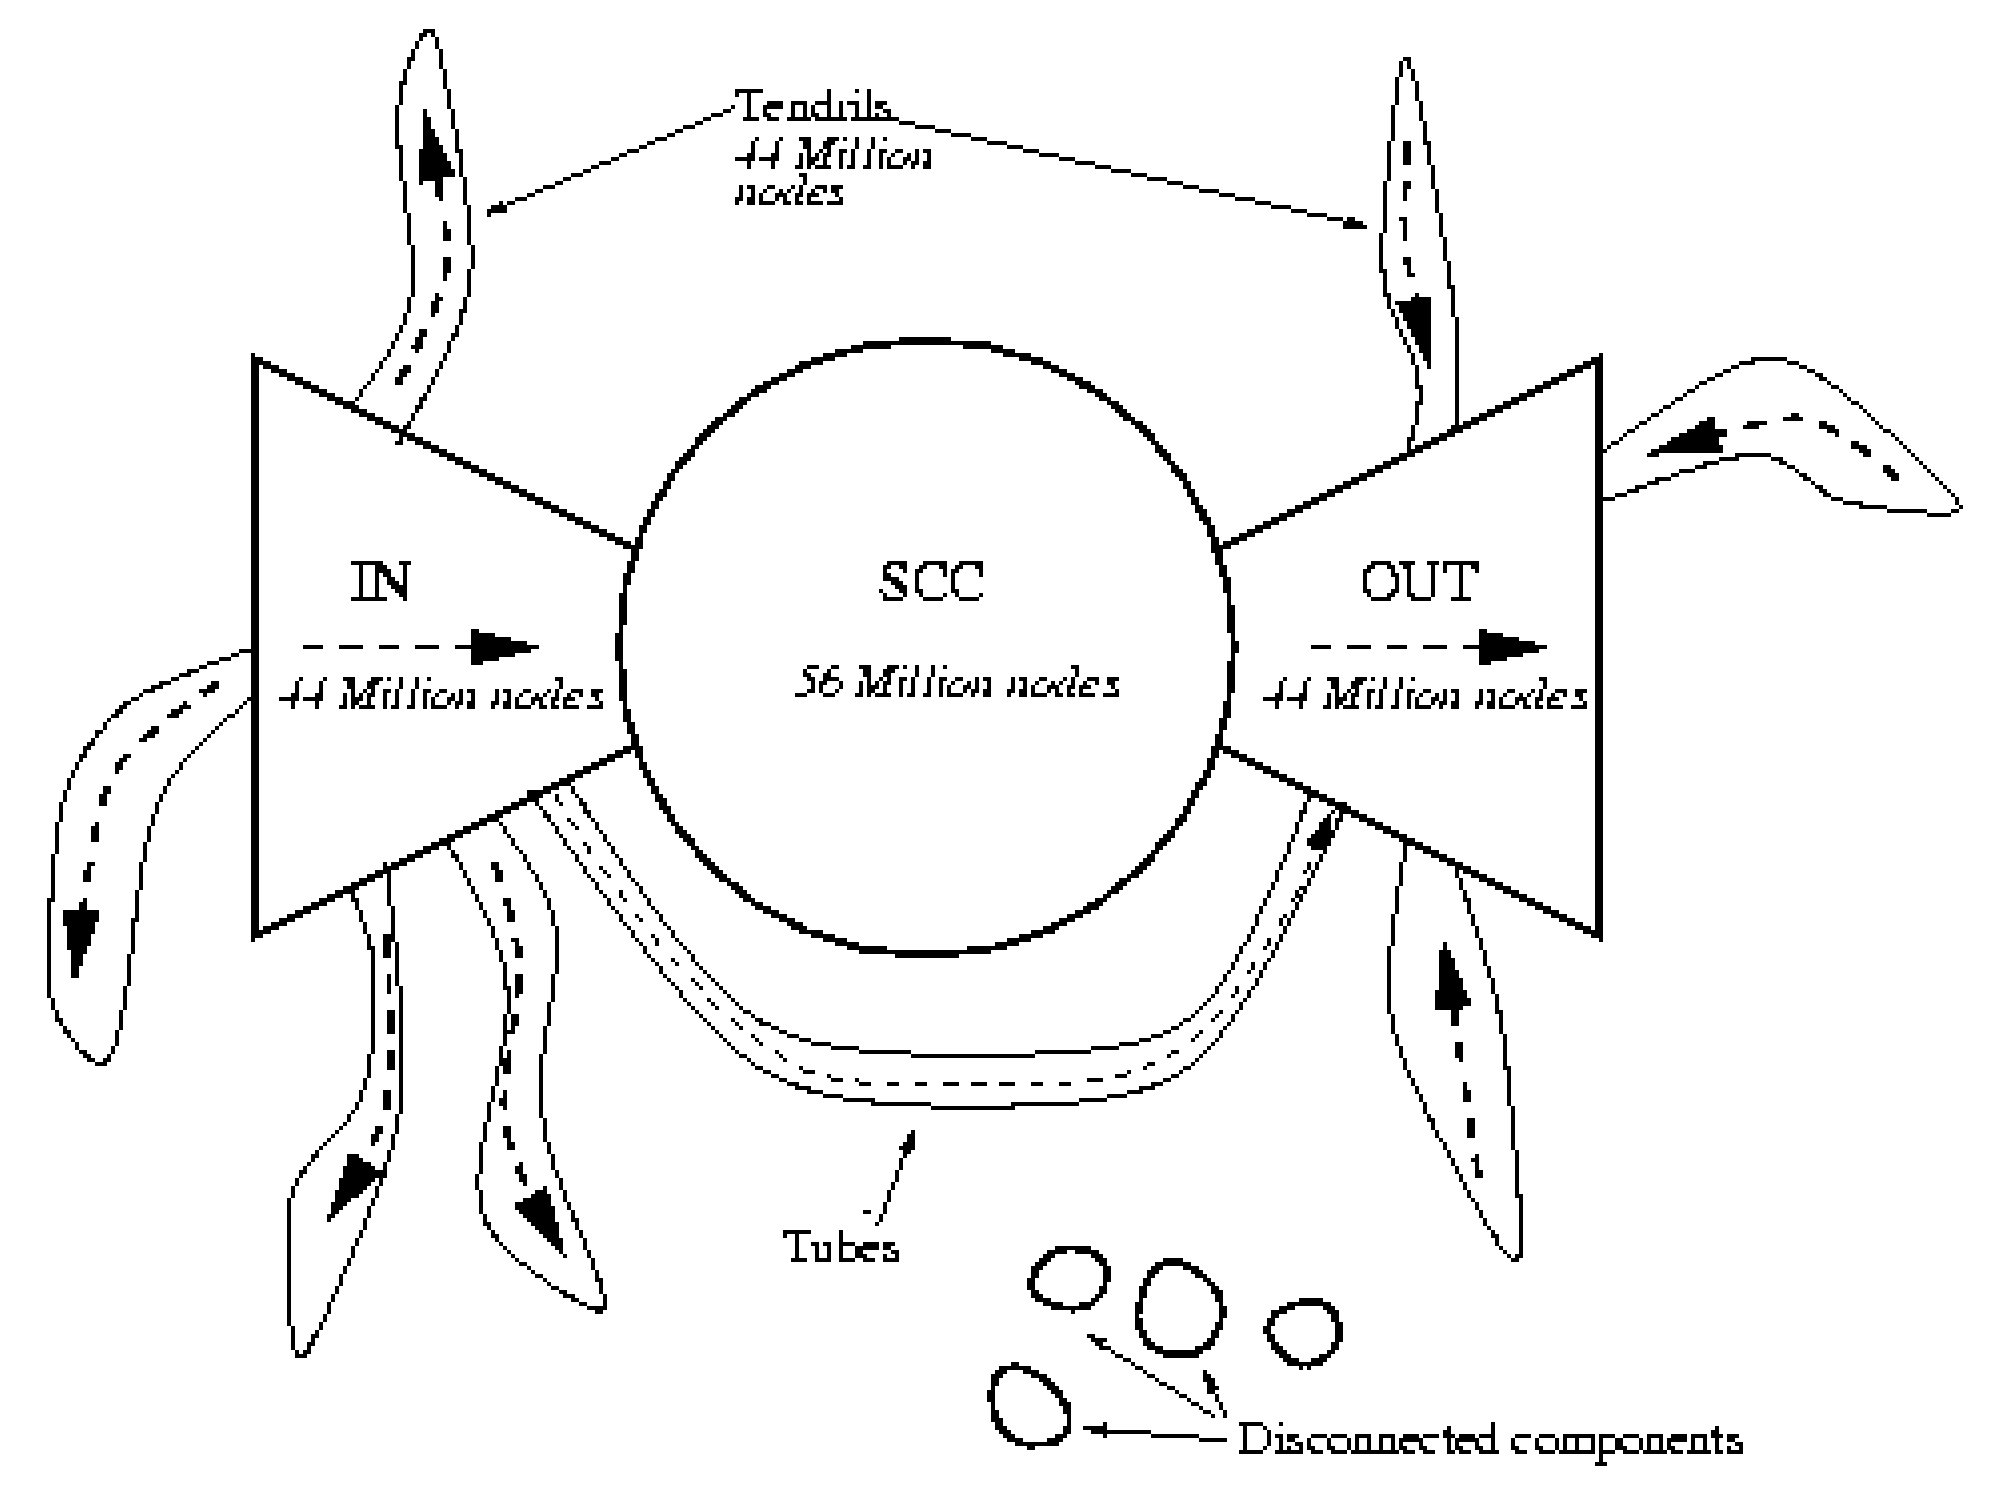
\includegraphics[scale = 0.5]{figs/web.png}
% \end{center}

% On repère trois composants principaux:
% \begin{itemize}
%  \item Un composant \textbf{in}, qui contient des liens hypertextes sortants.
%  \item Un composant fortement connecté principal, qui forme un \textbf{noyau} (SCC).
%  \item Un composant \textbf{out}, qui contient beaucoup de liens hypertextes entrants.
% \end{itemize}


% \newpage

% \section*{Exercices}


\subsection*{Exercice 1}
Considèrer de graphe avec 18 pages Web dans la Figure \ref{fig:webg}. Quels sont les noeuds qui font partie du noyau, les noeuds IN et les noeuds
OUT ? 

    \begin{figure}[h!]
    \begin{center}
    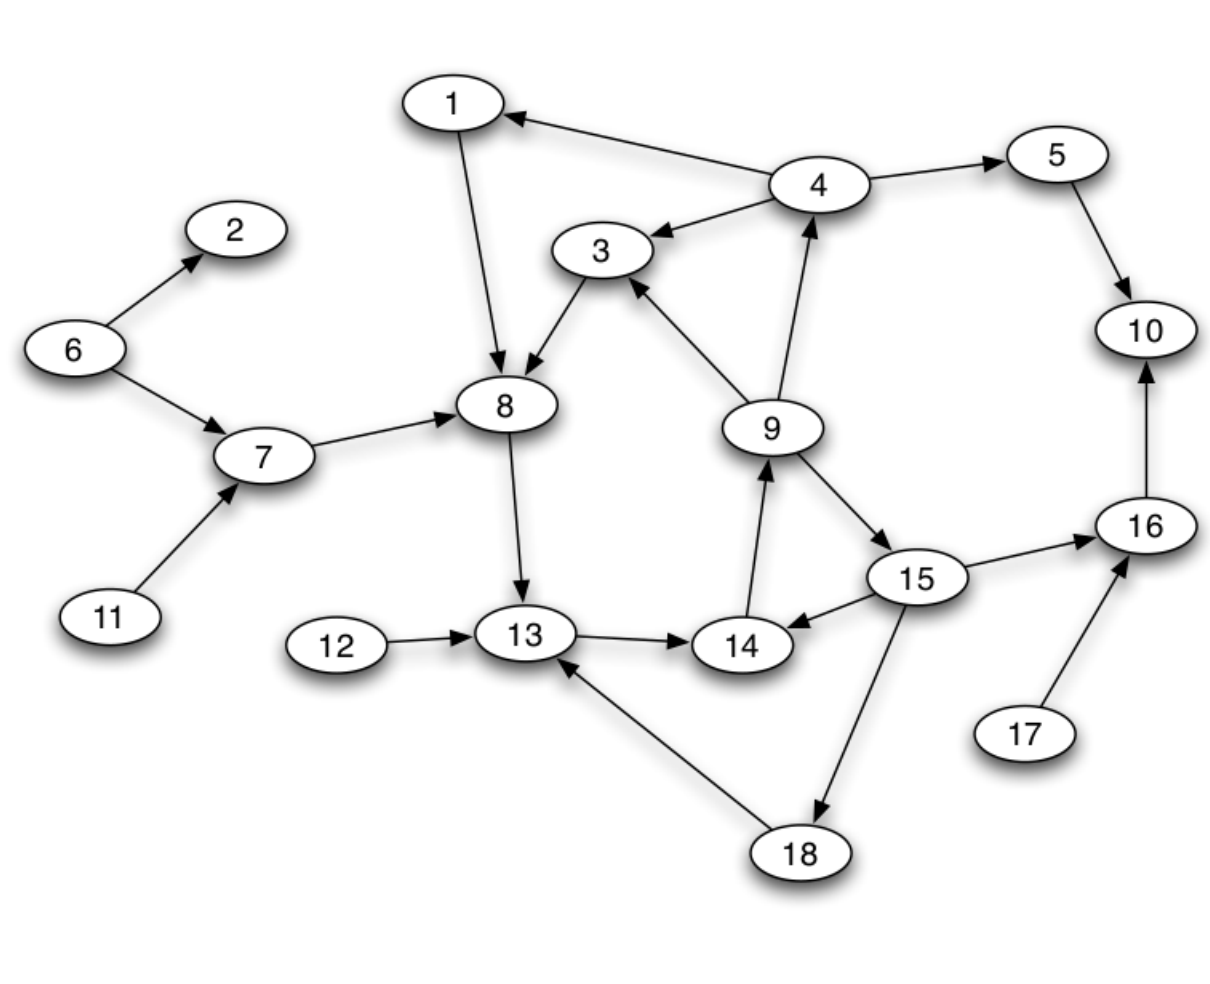
\includegraphics[scale = 0.3]{figs/graph.png}
    \end{center}
    \caption{Un graphe des pages web.}
    \label{fig:webg}
    \end{figure}

    \subsubsection*{Solution}

    \begin{center}
    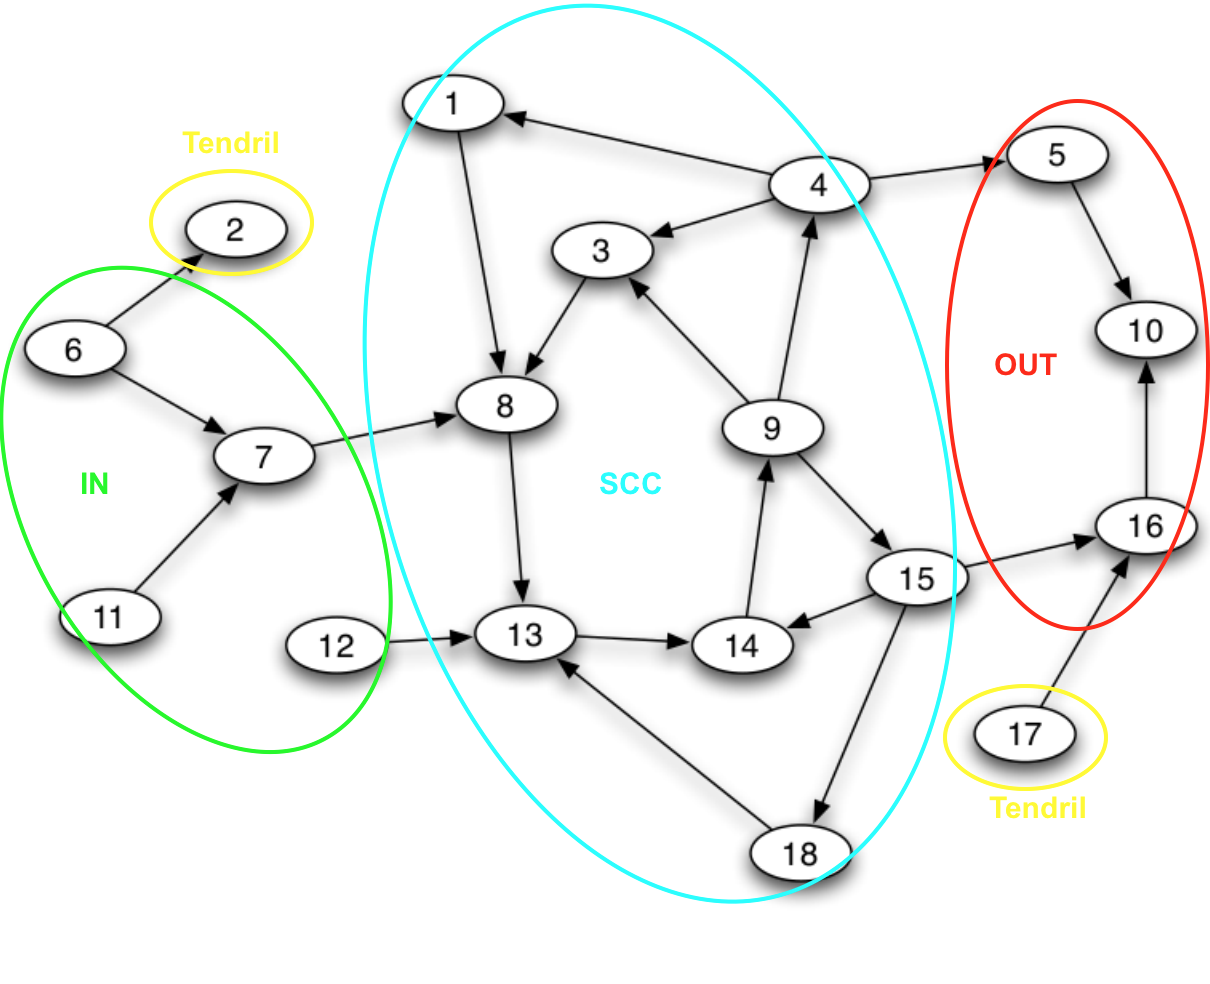
\includegraphics[scale=0.5]{pic/TP11Q1.png}
    \end{center}


\subsection*{Exercice 2}
Pour le graphe de la Figure \ref{fig:webg}.
\begin{enumerate}
 \item Montrez une arête tel que si on l'ajoute ou on la retire, on augmente la taille du noyau.
 \item Montrez une arête tel que si on l'ajoute ou on la retire, on augmente la taille de IN.
 \item Montrez une arête tel que si on l'ajoute ou on la retire, on augmente la taille de OUT.
\end{enumerate}

    \subsubsection*{Solution}

    \begin{center}
    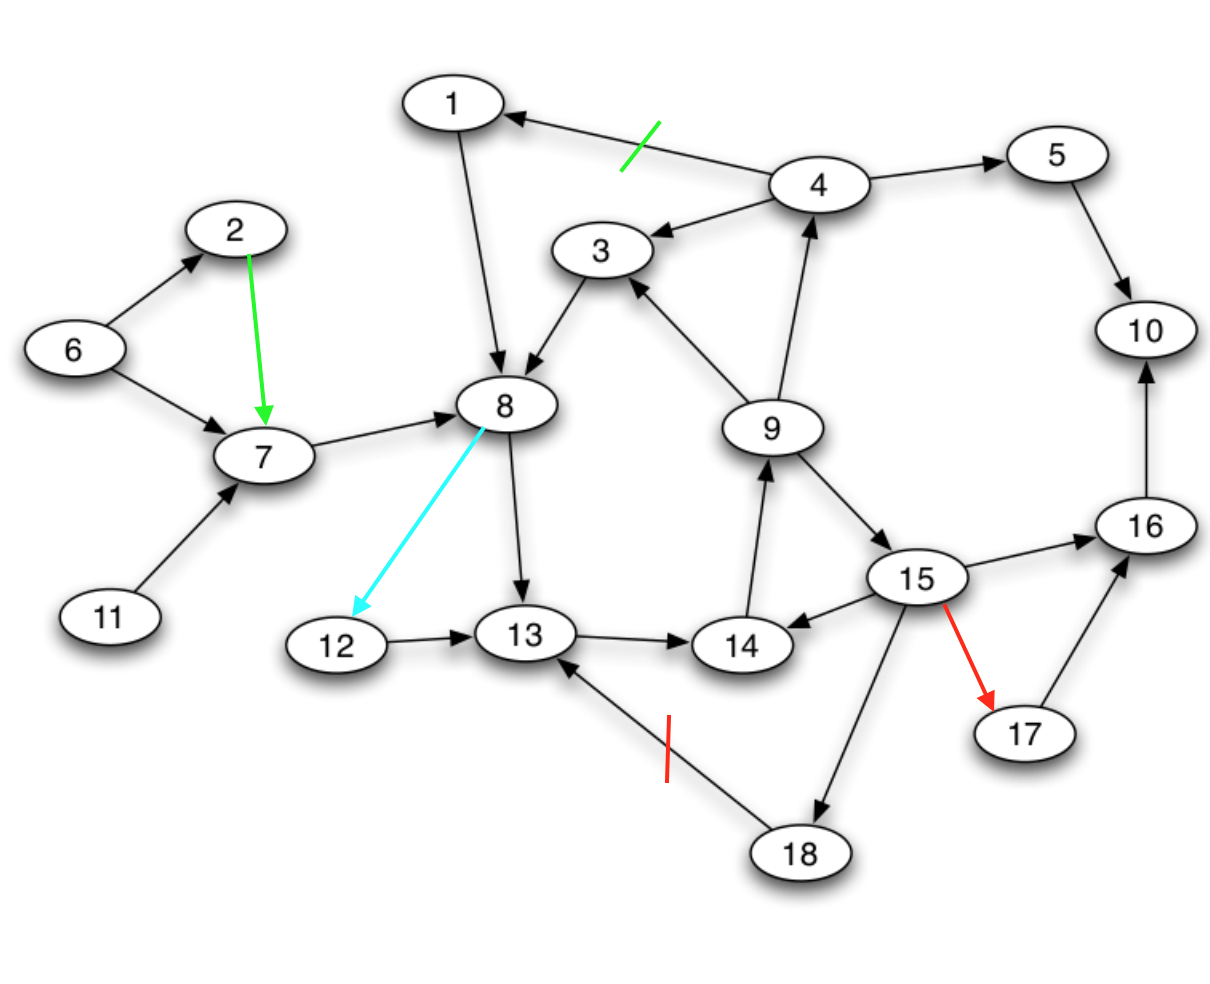
\includegraphics[scale=0.5]{pic/TP11Q2.png}
    \end{center}
    
    \begin{itemize}
        \item Le vert indique une arête à rajouter/retirer pour augmenter la taille du IN.
        \item Le rouge indique une arête à rajouter/retirer pour augmenter la taille du OUT.
        \item Le bleu indique une arête à rajouter pour augmenter la taille du SCC. Il n'est pas possible d'augmenter la taille du SCC en retirant une arête.
    \end{itemize}
    Il y a bien sûr d'autres possibilités que celles-là.


\subsection*{Exercice 3}
Décrivez un graphe tel qu'il existe une arête dont le retrait diminue la taille du noyeau d'au moins 1000 noeuds.

    \subsubsection*{Solution}
    Il faut pour cela un noyau qui possède un ensemble de 1000 noeuds ou plus qui n'est pas relié au IN ni au OUT et qui est relié au reste du noyau par seulement 2 arêtes : une entrante et une sortante.
    Supprimer l'arête qui va de cet ensemble au reste revient à rajouter l'ensemble au IN, tandis que supprimer l'autre arête revient à l'ajouter au OUT.


\subsection*{Exercice 4}
Décrivez un graphe tel qu'il existe une arête dont l'ajout diminue la taille de OUT d'au moins 1000 noueds.

    \subsubsection*{Solution}
    Il faut que le OUT possède une chaîne de 1000 noeuds ou plus et dont au moins un des noeuds de départ est directement lié au noyau.
    Il suffit de rajouter une arête au dernier noeud de cette chaîne pour qu'elle fasse partie intégrante du noyau, et donc pour diminuer la taille de OUT.

\subsection*{Exercice 5}
	\begin{enumerate}
	\item Calculez les valeurs de concentrateurs et d'autorités pour les pages dans le graphe présenté à la Figure \ref{fig:auth} après deux itérations.
	\item Quelles sont les valeurs une fois que la normalisation a été effectuée.
\end{enumerate}

\begin{figure}[!h]
	\centering
	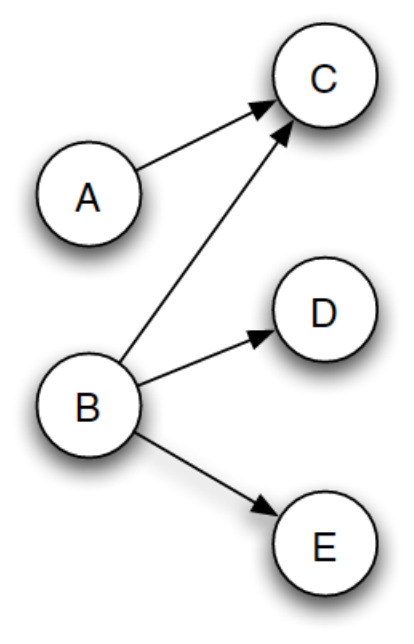
\includegraphics[scale=0.4]{figs/auth-hub.png}
	\caption{graphe de page web}
	\label{fig:auth}
\end{figure}

    \subsubsection*{Algorithme de normalisation}
    
    \begin{itemize}
        \item \textbf{Init} :  $ \forall x \: auth(x) = hub(x) = 1 $
        \item \textbf{Steps}: \\
            $\forall x \: auth(x) = \sum_{y \in hub(x)} hub(y)  $ \\
            $\forall x \: hub(x) = \sum_{y \in auth(x)} auth(y)  $
        \item \textbf{Normalisation} : \\
            $ \forall x \: auth(x) = \frac{auth(x)}{\sum auth} $ \\
            $ \forall x \: hub(x) = \frac{hub(x)}{\sum hub} $
    \end{itemize}

    \subsubsection*{Solution}
    \begin{itemize}
        \item \textbf{Auth} : authorité : liens entrants
        \item \textbf{Conc} : concentrateur : liens sortants
    \end{itemize}

    \begin{center}
    	\begin{tabular}{c|ccccc}
    	     & A & B & C & D & E\\ \hline
    	Auth & 1 & 1 & 1 & 1 & 1\\
    	Conc & 1 & 1 & 1 & 1 & 1\\ \hline
    	Auth & 0 & 0 & 2 & 1 & 1\\
    	Conc & 1 & 3 & 0 & 0 & 0\\ \hline
    	Auth & 0 & 0 & 4 & 3 & 3\\
    	Conc & 2 & 4 & 0 & 0 & 0\\ \hline
    	\end{tabular}
    \end{center}
    
    Normalisation :
    \begin{center}
    	\begin{tabular}{c|ccccc}
    	     & A & B & C & D & E\\ \hline
    	Auth & 0 & 0 & 0.4 & 0.3 & 0.3\\
    	Conc & $\frac{1}{3}$ & $\frac{2}{3}$ & 0 & 0 & 0\\ \hline
    	\end{tabular}
    \end{center}
    
    
\subsection*{Exercice 6}
Calculez les valeurs de PageRank pour chaque page dans le graphe présenté à la Figure \ref{fig:pagerank} après deux itérations avec S = 1.


\begin{figure}[ht!]
	\centering
	\begin{tikzpicture}[node distance=2cm]
		\tikzstyle{every node}=[draw=black,shape=circle]
		\node (c) at (0,0){C};
		\node[above of=c](a){A};
		\node[below of=c](e){E};
		\node[right of=c](d){D};
		\node[left of=c](b){B};

		\draw[->](a) -- (b);
		\draw[->](a) -- (d);
		\draw[->](b) -- (c);
		\draw[->](c) -- (a);
		\draw[->](c) -- (d);
		\draw[->](c) -- (e);
		\draw[->](d) -- (e);
		%\draw[->](d) -- (c);
		\draw[->](e) -- (b);
	\end{tikzpicture}
	\caption{graphe de page web}
	\label{fig:pagerank}
\end{figure}

    \subsubsection*{Solution}
    Règle de mise à jour : $Pr'(p) = S\ Pr(p) + (1-S) \frac{1}{n} = Pr(p)$.
    Seule la probabilité de suivre un lien à partir d'une page web entre en compte ici.\\
    À chaque itération k, on effectue les mises à jour suivantes :
    \begin{description}
        \item $Pr(A) = \frac{1}{3} Pr(C)$
        \item $Pr(B) = \frac{1}{2} Pr(A) + Pr(E)$
        \item $Pr(C) = Pr(B)$
        \item $Pr(D) = \frac{1}{2} Pr(A) + \frac{1}{3} Pr(C)$
        \item $Pr(E) = \frac{1}{3} Pr(C) + Pr(D)$
    \end{description}
    
    \begin{center}
        \begin{tabular}{c|ccccc}
        k & A & B & C & D & E\\ \hline 
    	0 & $\frac{1}{5}$ & $\frac{1}{5}$ & $\frac{1}{5}$ & $\frac{1}{5}$ & $\frac{1}{5}$\\ \\
    	1 & $\frac{1}{15}$ & $\frac{3}{10}$ & $\frac{1}{5}$ & $\frac{1}{6}$ & $\frac{4}{15}$\\ \\
    	2 & $\frac{1}{15}$ & $\frac{3}{10}$ & $\frac{3}{10}$ & $\frac{1}{10}$ & $\frac{7}{30}$\\
    	\end{tabular}
    \end{center}

\subsection*{Exercice 7}
Dans la Figure \ref{fig:equi}, les nombres à coté des noeuds représentent la valeur de PageRank de la page. Avec ce graphe, les valeurs de PageRank forment-elles un ensemble équilibré? Si oui pourquoi? Si non pourquoi?

\begin{figure}[ht!]
	\centering
	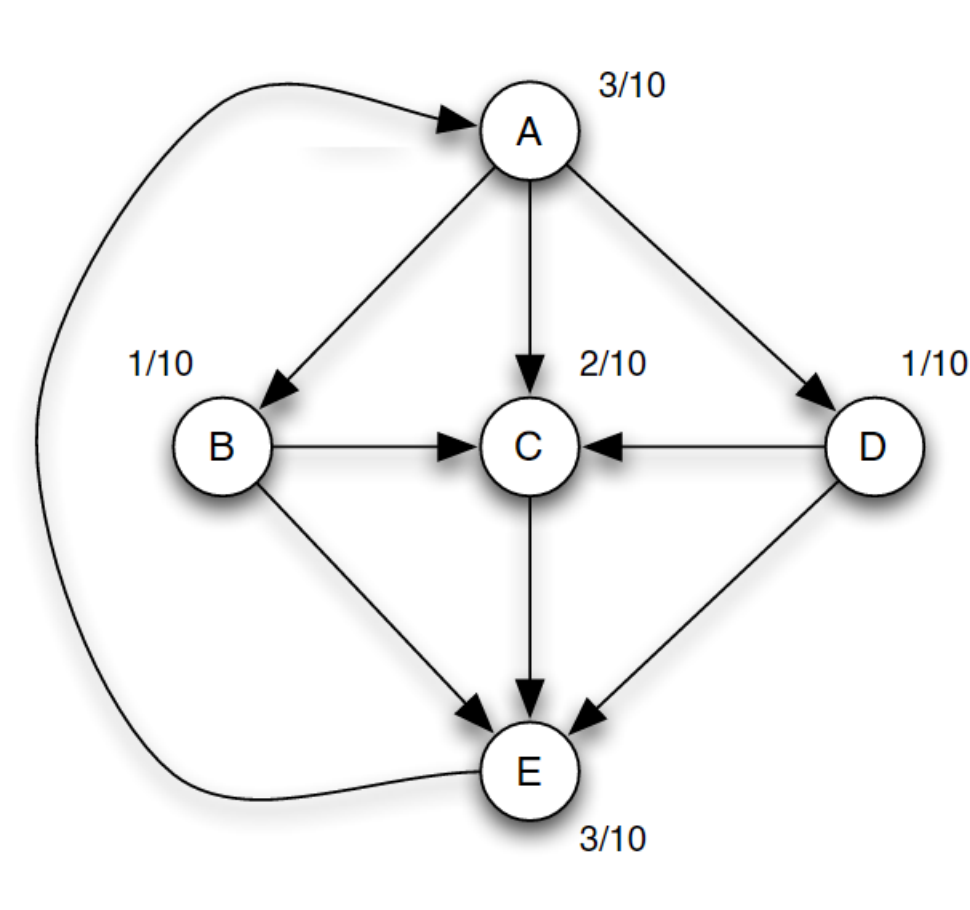
\includegraphics[scale=0.3]{figs/equi.png}
	\caption{graphe de page web}
	\label{fig:equi}
\end{figure}

    \subsubsection*{Solution}
    Il y a deux conditions à respecter pour que les valeurs de PageRank d'un graphe forment un ensemble équilibré :
    \begin{enumerate}
        \item La somme des valeurs doit valoir 1 : $\sum Pr(p_i) = 1$
        \item Une nouvelle itération doit donner les mêmes valeurs : $Pr'(p_i) = Pr(p_i) \ \forall p_i$\\
    \end{enumerate}
    
    Vérifions tout d'abord la première condition :
    $$ \sum Pr(p_i) = \frac{3}{10} + \frac{1}{10} + \frac{2}{10}  + \frac{1}{10}+  \frac{3}{10} = \frac{10}{10} = 1 $$

    Ensuite la seconde :
    \begin{description}
        \item $Pr'(A) = Pr(E) = \frac{3}{10} = Pr(A)$
        \item $Pr'(B) = \frac{1}{3} Pr(A) = \frac{1}{10} = Pr(B)$
        \item $Pr'(C) = \frac{1}{3} Pr(A) + \frac{1}{2} Pr(B) + \frac{1}{2} Pr(D) = \frac{2}{10} = Pr(C)$
        \item $Pr'(D) = \frac{1}{3} Pr(A) = \frac{1}{10} = Pr(D)$
        \item $Pr'(E) = \frac{1}{2} Pr(B) + Pr(C) + \frac{1}{2} Pr(D) = \frac{3}{10} = Pr(E)$\\
    \end{description}

    Nous pouvons donc conclure que nous cet ensemble de valeurs PageRank forme bien un ensemble équilibré.
    

\subsection*{Exercice 8}
		\begin{enumerate}
				\item Calculez les valeurs de PageRank pour chaque page dans le graphe présenté à la Figure \ref{fig:blackhole} après trois itérations avec S = 1.
				\item Que remarquez-vous? Selon vous comment vont évoluer les valeurs
						de PageRank pour un nombre d'itérations de plus en plus grand
				\item Calculez à nouveau les valeurs de PageRank pour chaque page mais pour 2 itérations avec S = 0.5.
		\end{enumerate}
		
    \begin{figure}[ht!]
	\centering
	
\begin{tikzpicture}[node distance=2cm]
	\tikzstyle{every node}=[draw=black,shape=circle]
	\node (c) at (0,0){C};
	\node[above of=c](a){A};
	\node[below of=c](e){E};
	\node[right of=c](d){D};
	\node[left of=c](b){B};

	\draw[->](a) -- (b);
	\draw[->](a) -- (d);
	\draw[->](b) -- (c);
	\draw[->](c) -- (a);
	\draw[->](c) -- (d);
	\draw[->](c) -- (e);
	\draw[->](d) -- (e);
	%\draw[->](d) -- (c);
	%\draw[->](e) -- (b);
\end{tikzpicture}
\caption{graphe de page web}
\label{fig:blackhole}
\end{figure}
		
    \subsubsection*{Solution}
    Pour S=1, à chaque itération k, on effectue les mises à jour suivantes :
    \begin{description}
        \item $Pr(A) = \frac{1}{3} Pr(C)$
        \item $Pr(B) = \frac{1}{2} Pr(A)$
        \item $Pr(C) = Pr(B)$
        \item $Pr(D) = \frac{1}{2} Pr(A) + \frac{1}{3} Pr(C)$
        \item $Pr(E) = \frac{1}{3} Pr(C) + Pr(D) + Pr(E)$ \\
        \textit{(On ajoute $Pr(E)$ au calcul de E car c'est un noeud "cul-de-sac". Lors d'une itération, il faut prendre en compte le fait qu'une transition est bloquée au niveau de E et retombera donc vers E.)}
    \end{description}
    
    On obtient le résultat qui suit :
    \begin{center}
        \begin{tabular}{c|ccccc}
        k & A & B & C & D & E\\ \hline 
    	0 & $\frac{6}{30}$ & $\frac{6}{30}$ & $\frac{6}{30}$ & $\frac{6}{30}$ & $\frac{6}{30}$\\ \\
    	1 & $\frac{2}{30}$ & $\frac{3}{30}$ & $\frac{6}{30}$ & $\frac{5}{30}$ & $\frac{14}{30}$\\ \\
    	2 & $\frac{2}{30}$ & $\frac{1}{30}$ & $\frac{3}{30}$ & $\frac{3}{30}$ & $\frac{21}{30}$\\ \\
    	3 & $\frac{1}{30}$ & $\frac{1}{30}$ & $\frac{1}{30}$ & $\frac{2}{30}$ & $\frac{25}{30}$\\
    	\end{tabular}
    \end{center}
    
    On remarque qu'il y a une accumulation au niveau du noeud E.
    Sa valeur va tendre vers 1 alors que toutes les autres tendent vers 0.
    
    Pour S=0.5, à chaque itération k, on effectue les mises à jour suivantes :
    \begin{description}
        \item $Pr'(A) = \frac{1}{6} Pr(C) + \frac{1}{10}$
        \item $Pr'(B) = \frac{1}{4} Pr(A) + \frac{1}{10}$
        \item $Pr'(C) = \frac{1}{2} Pr(B) + \frac{1}{10}$
        \item $Pr'(D) = \frac{1}{4} Pr(A) + \frac{1}{6} Pr(C) + \frac{1}{10}$
        \item $Pr'(E) = \frac{1}{6} Pr(C) + \frac{1}{2} Pr(D) + \frac{1}{2} Pr(E) + \frac{1}{10}$
    \end{description}
    
    Le tableau résultant est :
    \begin{center}
        \begin{tabular}{c|ccccc}
        k & A & B & C & D & E\\ \hline 
    	0 & $\frac{6}{30}$ & $\frac{6}{30}$ & $\frac{6}{30}$ & $\frac{6}{30}$ & $\frac{6}{30}$\\ \\
    	1 & $\frac{4}{30}$ & $\frac{4.5}{30}$ & $\frac{6}{30}$ & $\frac{5.5}{30}$ & $\frac{10}{30}$\\ \\
    	2 & $\frac{4}{30}$ & $\frac{4}{30}$ & $\frac{5.25}{30}$ & $\frac{5}{30}$ & $\frac{11.75}{30}$\\
    	\end{tabular}
    \end{center}



  
  %Quid de ca? 
    %\include{references}

\end{document}
